% 单文件讲义；最新版本在桌面“数字逻辑设计讲义”文件夹维护。
% 新增正文放在“主要结论与术语”之前，并同步更新资料说明。
\documentclass[UTF8,fontset=none,zihao=-4,a4paper]{ctexart}
\usepackage[left=26mm,right=26mm,top=25mm,bottom=25mm,headheight=16pt]{geometry}
% ---------- 字体集中定义 ----------
\IfFontExistsTF{Songti SC}{
 \setCJKmainfont{Songti SC}[BoldFont={Songti SC Bold}]
 \setCJKsansfont{Songti SC}[BoldFont={Songti SC Bold}]
 \setCJKmonofont{Songti SC}[BoldFont={Songti SC Bold}]
}{
 \setCJKmainfont{FandolSong-Regular.otf}[BoldFont={FandolSong-Bold.otf}]
 \setCJKsansfont{FandolSong-Regular.otf}[BoldFont={FandolSong-Bold.otf}]
 \setCJKmonofont{FandolSong-Regular.otf}[BoldFont={FandolSong-Bold.otf}]
}
\IfFontExistsTF{Times New Roman}{
 \setmainfont{Times New Roman}\setsansfont{Times New Roman}\setmonofont{Times New Roman}
}{
 \setmainfont{texgyretermes-regular.otf}[BoldFont={texgyretermes-bold.otf},ItalicFont={texgyretermes-italic.otf}]
 \setsansfont{texgyretermes-regular.otf}[BoldFont={texgyretermes-bold.otf}]
 \setmonofont{texgyretermes-regular.otf}[BoldFont={texgyretermes-bold.otf}]
}
\usepackage{amsmath,amssymb,booktabs,tabularx,array,longtable,enumitem,fancyhdr,needspace}
\usepackage{unicode-math}\setmathfont{texgyretermes-math.otf}
% Code identifiers and listings use a monospaced Latin font.
\IfFontExistsTF{Menlo}{\setmonofont{Menlo}}{
 \IfFontExistsTF{Courier New}{\setmonofont{Courier New}}{\setmonofont{lmmono10-regular.otf}}
}
\usepackage{xcolor,tikz,listings}
\usetikzlibrary{arrows.meta,positioning,automata,calc,shapes.gates.logic.US}
\usepackage[breakable,skins]{tcolorbox}
\usepackage[hidelinks]{hyperref}
\hypersetup{pdftitle={数字逻辑设计},pdfsubject={课程理论与数字逻辑实验代码讲解}}
% ---------- 配色和信息框集中定义 ----------
\definecolor{ThemeMain}{HTML}{35566E}
\definecolor{ThemeBack}{HTML}{F2F6F8}
\definecolor{ThemeBorder}{HTML}{B8C8D3}
\newtcolorbox{infobox}[2][]{enhanced,breakable,colback=ThemeBack,
 colframe=ThemeBorder,colbacktitle=ThemeBack,coltitle=ThemeMain,
 fonttitle=\normalsize\bfseries,title={#2},attach title to upper={\par\smallskip},
 boxrule=0.45pt,arc=0.8mm,left=3mm,right=3mm,top=2mm,bottom=2mm,
 before skip=7pt,after skip=7pt,pad at break*=1.5mm,#1}
\lstset{language=Verilog,basicstyle=\fontsize{10.5}{12.6}\selectfont\ttfamily,keywordstyle=\color{ThemeMain}\bfseries,
 commentstyle=\color{ThemeMain},stringstyle=\color{black},columns=fullflexible,
 keepspaces=true,showstringspaces=false,breaklines=true,breakatwhitespace=false,
 frame=single,rulecolor=\color{ThemeBorder},backgroundcolor=\color{ThemeBack},
 framerule=0.4pt,xleftmargin=2mm,xrightmargin=2mm,framesep=2mm,
 aboveskip=8pt,belowskip=8pt,tabsize=2}
\tikzset{>=Stealth,every node/.style={font=\small},block/.style={draw=ThemeMain,
 fill=ThemeBack,minimum height=11mm,align=center},state/.style={circle,draw=ThemeMain,
 fill=ThemeBack,minimum size=12mm},every edge/.style={draw=ThemeMain,->}}
% ---------- 正文、标题与页码 ----------
\ctexset{section={format=\large\bfseries,beforeskip=0pt,afterskip=14pt},
 subsection={format=\normalsize\bfseries,beforeskip=10pt,afterskip=5pt},
 subsubsection={format=\normalsize\bfseries,beforeskip=8pt,afterskip=4pt}}
\setcounter{tocdepth}{1}\setcounter{secnumdepth}{2}
\linespread{1.22}\setlength{\parindent}{2em}\setlength{\parskip}{2pt}
\setlength{\tabcolsep}{5pt}\renewcommand{\arraystretch}{1.20}
\setlength{\emergencystretch}{1.5em}\allowdisplaybreaks[2]\raggedbottom
\setlist{itemsep=3pt,topsep=4pt,parsep=0pt,leftmargin=2em}
\setlist[enumerate]{label=\arabic*.}
\pagestyle{fancy}\fancyhf{}
\fancyhead[L]{\small 数字逻辑设计}
\fancyhead[R]{\small\nouppercase{\leftmark}}
\fancyfoot[C]{\small\thepage}\renewcommand{\headrulewidth}{0.3pt}
\renewcommand{\sectionmark}[1]{\markboth{#1}{}}
\newcommand{\chapterpage}[1]{\clearpage\section{#1}}
\newcommand{\term}[1]{\textbf{#1}}
\newcommand{\sol}{\par\noindent\textbf{解}\quad}
\newcommand{\code}[1]{\allowbreak{\small\texttt{\detokenize{#1}}}\allowbreak}
\newcolumntype{Y}{>{\raggedright\arraybackslash}X}
\begin{document}
\begin{titlepage}\thispagestyle{empty}\vspace*{0.28\textheight}
\begin{center}{\fontsize{36}{45}\selectfont\bfseries 数字逻辑设计}\end{center}
\end{titlepage}
\pagenumbering{Roman}\thispagestyle{empty}
\begingroup\linespread{1.05}\selectfont\tableofcontents\endgroup\clearpage
\pagenumbering{arabic}

\section{数字系统与逻辑抽象}
\subsection{数字信号、模拟信号与二值逻辑}
\term{数字逻辑设计}（Digital Logic Design）研究以离散代码表示信息、以逻辑电路处理和存储信息的方法。\term{模拟信号}的幅值可在一定区间连续取值；\term{数字信号}用有限个规定的信号状态表示代码。实际导线上的电压仍是连续的物理量，逻辑分析只把处于规定电平区间的电压解释为逻辑值。

数字电路常采用\term{二值逻辑}：变量取 $0$ 或 $1$。二进制适合由截止、导通等两种主要工作状态的开关器件实现。二极管具有单向导电性；双极型晶体管可利用截止和饱和状态实现开关；集成电路把器件和互连集中在芯片内。逻辑门在抽象层面完成逻辑运算，具体电气实现还须满足供电、门限及负载要求。

\begin{infobox}{定义：电平与逻辑值}
\term{正逻辑}把高电平解释为 $1$、低电平解释为 $0$；负逻辑采用相反的对应。逻辑值不是电压的数值本身。电平有效性应按器件规定的输入、输出电压范围判断，处于未定义区间的输入不能可靠地解释为 $0$ 或 $1$。
\end{infobox}
数字信号的抗干扰能力来自电平区间与门限之间的余量，并非能够抵抗任意噪声。数字信号也不必仅在离散时刻变化；同步系统在时钟边沿采样、更新状态，而异步输入可以在任意时刻变化。

\subsection{信息转换与分辨率}
模拟物理量进入数字系统通常经历采样、量化和编码；\term{模数转换}（A/D）把模拟输入转换为数字代码，\term{数模转换}（D/A）把代码转换为相应的模拟输出。数字系统适于存储、复制、运算和可编程控制，但接口的转换误差仍会影响最终结果。

设转换位数为 $n$，可表示 $2^n$ 个等级。若 A/D 输入范围的宽度为 $V_{\mathrm{FS}}$，均匀量化模型中一个量化间隔为
\[
\Delta V=\frac{V_{\mathrm{FS}}}{2^n}.
\]
课件把相对分辨率写为 $1/2^n$。若 D/A 的最大码对应输出 $V_{\max}$，并把最小码输出取为零，则从零码到满码有 $2^n-1$ 个间隔，课件对应的相对步长为 $1/(2^n-1)$。若另把标称满量程定义为 $2^n$ 个步长，也会出现 $1/2^n$ 的 D/A 分辨率表达式。比较不同资料时须先统一满量程的定义。

\begin{infobox}{例题：8位均匀量化}
A/D 输入范围为 $0$ 至 $5\,\mathrm{V}$，位数为 $8$，求理想量化间隔。
\end{infobox}
\sol $\Delta V=5/256\,\mathrm{V}\approx19.53\,\mathrm{mV}$。该结果描述理想分辨能力，不等于实际转换精度；偏移、非线性与噪声均可能造成额外误差。

\subsection{组合逻辑、时序逻辑与设计层次}
\term{组合逻辑电路}在输入稳定并经过传播延迟后，输出只由当前输入决定：
\[
\symbf{Z}=f(\symbf{X}).
\]
\term{时序逻辑电路}具有存储状态，输出和次态由输入及现态确定：
\[
\symbf{Q}^{+}=g(\symbf{Q},\symbf{X}),\qquad
\symbf{Z}=h(\symbf{Q},\symbf{X}).
\]
其中 $\symbf{X}$ 是输入向量，$\symbf{Z}$ 是输出向量，$\symbf{Q}$ 是现态，$\symbf{Q}^{+}$ 是次态。上标 $+$ 表示下一次状态更新后的值，并非算术加法。

设计可分为三个层次：系统设计划分功能模块并确定接口；逻辑设计利用门、触发器及功能部件实现模块；电路设计确定器件、电气连接与物理实现。硬件描述语言描述结构和行为，电子设计自动化工具辅助仿真、综合、布局布线和时序分析。
\begin{center}

\begin{tikzpicture}[node distance=7mm]
\node[block,text width=25mm] (a) {需求与接口};
\node[block,text width=25mm,right=of a] (b) {组合逻辑\\与状态存储};
\node[block,text width=25mm,right=of b] (c) {仿真、综合\\与物理实现};
\node[block,text width=25mm,right=of c] (d) {时序与功能\\验证};
\draw[->,ThemeMain] (a)--(b);\draw[->,ThemeMain] (b)--(c);\draw[->,ThemeMain] (c)--(d);
\end{tikzpicture}
\end{center}

\subsection{集成规模与可编程逻辑器件}
小规模、中规模、大规模和超大规模集成电路分别常记作 SSI、MSI、LSI、VLSI。门数划分随技术和统计口径变化，课件给出的范围用于说明规模层次，不作为所有技术通用的严格边界。

\term{可编程逻辑器件}（PLD）通过配置改变逻辑功能。常见类别有可编程阵列逻辑 PAL、复杂可编程逻辑器件 CPLD，以及现场可编程门阵列 FPGA。它们把门、查找表、触发器和可编程互连等资源组合成指定电路。资源结构将在组合逻辑器件一章中讨论。

\subsection{由分辨率指标确定转换位数}
\begin{infobox}{例题：按量化间隔选取A/D位数}
依据课件02第3页的均匀量化模型。A/D输入范围为 $0$ 至 $3.3\,\mathrm V$，要求量化间隔不大于 $2\,\mathrm{mV}$。求满足要求的最少位数，并核对相邻两种位数。
\end{infobox}
\sol 输入范围宽度为 $V_{\mathrm{FS}}=3.3\,\mathrm V$，指标须先统一单位：$2\,\mathrm{mV}=0.002\,\mathrm V$。由 $\Delta V=V_{\mathrm{FS}}/2^n$ 得
\[
\frac{3.3}{2^n}\le0.002
\quad\Longleftrightarrow\quad 2^n\ge1650.
\]
由于 $2^{10}=1024<1650\le2048=2^{11}$，最少须取 $n=11$。逐一核对：
\[
\Delta V_{10}=\frac{3.3}{1024}\,\mathrm V\approx3.223\,\mathrm{mV},\qquad
\Delta V_{11}=\frac{3.3}{2048}\,\mathrm V\approx1.611\,\mathrm{mV}.
\]
十位不满足要求，十一位满足要求。位数应向上取整，不能把对数结果四舍五入后直接选型；本题只约束理想量化间隔，没有给出实际转换误差指标。


\chapterpage{数制与编码}
\subsection{位权、基数与数值表示}
\term{按位计数制}中，每一位数符的意义由其位置和基数共同决定。设基数为 $r\ge2$，整数部分有 $p$ 位，小数部分有 $n$ 位，则
\begin{infobox}{公式：按位展开}
\[
(d_{p-1}\cdots d_0.d_{-1}\cdots d_{-n})_r
=\sum_{i=-n}^{p-1}d_i r^i,\qquad 0\le d_i<r.
\]
$r^i$ 是第 $i$ 位的\term{权}，$d_i$ 是该位数符的数值。二、八、十、十六进制的基数分别为 $2,8,10,16$。
\end{infobox}
十六进制数符 $\mathrm{A,B,C,D,E,F}$ 分别表示十进制 $10$ 至 $15$。\term{最高有效位}（MSB）是位权最大的位，\term{最低有效位}（LSB）是位权最小的位。固定宽度整数有前导零时，这两个名称仍指指定字中的最高、最低位置。

\subsection{十进制与其他进制的转换}
整数转换采用\term{除基取余、逆序排列}。反复用 $r$ 除整数，先得到的余数是最低位；商为零后，将余数倒序排列。依据为 $N=r\lfloor N/r\rfloor+(N\bmod r)$。

小数转换采用\term{乘基取整、顺序排列}。设当前小数为 $x$，计算 $rx=d+x'$，其中 $d=\lfloor rx\rfloor$、$0\le x'<1$；$d$ 是下一位数符，对 $x'$ 重复操作。余下小数为零时结束；若不结束，按所需位数截断或舍入。
\begin{infobox}{例题：十进制数转换为二进制}
把 $(87.4375)_{10}$ 转换为二进制。
\end{infobox}
\sol 整数部分的连续商为 $43,21,10,5,2,1,0$，对应余数为 $1,1,1,0,1,0,1$，逆序得到 $1010111$。小数部分为
\begin{align*}
0.4375\times2&=0.875 &&\text{取 }0,\\
0.875\times2&=1.75 &&\text{取 }1,\\
0.75\times2&=1.5 &&\text{取 }1,\\
0.5\times2&=1.0 &&\text{取 }1.
\end{align*}
故 $(87.4375)_{10}=(1010111.0111)_2$。

有限十进制小数不一定是有限二进制小数。约分后的分母仅含因子 $2$ 时，才能用有限二进制小数精确表示；例如 $1/10$ 的二进制展开无限循环。保留 $k$ 位二进制小数并截断时，绝对误差小于 $2^{-k}$。

\subsection{二、八、十六进制的分组转换}
因为 $8=2^3$、$16=2^4$，一位八进制数对应三位二进制，一位十六进制数对应四位二进制。以小数点为边界，整数向左、小数向右分组；整数最左端和小数最右端可补零，不能在其他位置随意补零。
\[
(10111000.1101)_2=(270.64)_8=(\mathrm{B8.D})_{16}.
\]
八进制小数 $0.64$ 对应 $0.110100$，末尾零不改变值。分组仅改变表示方式，不改变数值。

\subsection{二进制编码、BCD与有权码}
\term{编码}给对象分配代码。数制规定代码的数值解释，码制规定代码与对象的对应。$n$ 位二进制有 $2^n$ 个不同码字，给 $N$ 个对象分配互不相同的等长码字须满足 $2^n\ge N$。

\term{二—十进制编码}（BCD，Binary-Coded Decimal）用四位二进制代码表示一位十进制数码。\term{8421 BCD码}的四位权值为 $8,4,2,1$；仅使用 $0000$ 至 $1001$，其余六个码字不是有效十进制数码。
\[
(59)_{10}\longleftrightarrow(0101\ 1001)_{\mathrm{BCD}},\qquad
(59)_{10}=(111011)_2.
\]
BCD 的分组应按十进制数码处理，不能把整串 BCD 当作普通二进制数。

\term{有权码}的数值等于各位权值之和，但仅给权值不一定能唯一确定码表。例如 2421 码中 $0101$ 与 $1011$ 的位权和都为 $5$，必须约定选用哪一个码字。下表采用课件的非括号方案。
\begin{center}
\begin{tabular}{c c c c c c}
\toprule 十进制 & 8421 & 2421 & 4221 & 5421 & 余3码\\\midrule
0&0000&0000&0000&0000&0011\\
1&0001&0001&0001&0001&0100\\
2&0010&0010&0010&0010&0101\\
3&0011&0011&0011&0011&0110\\
4&0100&0100&0110&0100&0111\\
5&0101&1011&1001&1000&1000\\
6&0110&1100&1100&1001&1001\\
7&0111&1101&1101&1010&1010\\
8&1000&1110&1110&1011&1011\\
9&1001&1111&1111&1100&1100\\\bottomrule
\end{tabular}
\end{center}
\term{余3码}（Excess-3）把每个十进制数码 $d$ 编为四位二进制的 $d+3$，有效码范围为 $0011$ 至 $1100$。它是无权码；四个位不能直接按固定权相加得到原十进制数码。表中的 2421 码及余3码具有自补性质：某数码代码逐位取反后，对应 $9-d$。

\subsection{典型格雷码及相互转换}
\term{格雷码}（Gray Code）使相邻码字只相差一位。课程使用\term{二进制反射格雷码}；完整码表的首尾也仅相差一位。其编号顺序与普通二进制不同。
\begin{infobox}{方法：二进制与典型格雷码互换}
设二进制为 $b_{n-1}\cdots b_0$，格雷码为 $g_{n-1}\cdots g_0$。
\[
g_{n-1}=b_{n-1},\qquad g_i=b_{i+1}\oplus b_i\quad(0\le i<n-1).
\]
反向转换从最高位开始累积异或：
\[
b_{n-1}=g_{n-1},\qquad b_i=b_{i+1}\oplus g_i.
\]
$\oplus$ 表示异或，两位不同时结果为 $1$。
\end{infobox}
反射构造法从一位表 $0,1$ 开始：旧表正序前加 $0$，旧表逆序前加 $1$，合并成下一位宽的码表。三位典型格雷码依次为
\[
000,001,011,010,110,111,101,100.
\]
二进制 $1011$ 对应格雷码 $1110$。格雷码改变一位的性质有助于减少连续位置变化时的混合码错误，也用于卡诺图排列；它不能保证任意跳变均只有一位变化。

\begin{infobox}{例题：余3码转换为格雷码}
给定两个十进制数码的余3码 $1001\ 0101$，求其数值对应的典型格雷码。
\end{infobox}
\sol 两组码分别表示 $9-3=6$ 与 $5-3=2$，故数值为 $62$。若整数采用八位二进制，$62=00111110_2$，对应八位格雷码 $00100001$。若按每个数码分别编码，则 $6=0110_2\mapsto0101$、$2=0010_2\mapsto0011$，结果为 $0101\ 0011$。码制转换题须明确整值还是逐数码转换以及输出位宽。

\subsection{字符编码}
\term{ASCII}把控制字符、数字、拉丁字母等映射为字符代码。标准 ASCII 是七位编码，共 $128$ 个代码，常存放在最高位为零的八位字节中；课件中“8位”应理解为常见存储宽度。字符 \code{0}、\code{A}、\code{a} 的代码分别为十进制 $48,65,97$，即十六进制 $30,41,61$。字符 \code{0} 的代码不等于数值零。

GB2312、GBK、GB18030 是中文字符编码方案；Unicode 为字符分配统一码点，UTF-8 等编码形式规定码点如何转换为字节序列。字符、码点和存储字节须区分。ASCII 位数依据 \href{https://www.rfc-editor.org/rfc/rfc20}{RFC 20}核对。

\subsection{有限位小数与格雷码的计算}
\begin{infobox}{例题：无限二进制小数的八位截断}
按课件02第7页的乘基取整方法，将 $(0.1)_{10}$ 转为二进制小数，保留八位并截断。求所表示的十进制值及截断误差。
\end{infobox}
\sol 每次乘 $2$，整数部分成为下一位，余下小数继续计算：
\begin{center}
\begin{tabular}{c c c c}
\toprule 步数 & 当前小数乘 $2$ & 取出的位 & 剩余小数\\\midrule
1&$0.1\times2=0.2$&0&0.2\\
2&$0.2\times2=0.4$&0&0.4\\
3&$0.4\times2=0.8$&0&0.8\\
4&$0.8\times2=1.6$&1&0.6\\
5&$0.6\times2=1.2$&1&0.2\\
6&$0.2\times2=0.4$&0&0.4\\
7&$0.4\times2=0.8$&0&0.8\\
8&$0.8\times2=1.6$&1&0.6\\\bottomrule
\end{tabular}
\end{center}
余下小数再次出现 $0.2$，后续位会循环，故不能得到有限的精确表示。八位截断结果及其数值为
\[
(0.00011001)_2=2^{-4}+2^{-5}+2^{-8}
=\frac{25}{256}=0.09765625.
\]
以“原数减截断值”定义误差，则
\[
e=0.1-0.09765625=0.00234375<2^{-8}=0.00390625.
\]
截断与舍入是不同规则；本题不依据第九位进位。给定位数后，仍须说明采用哪一种规则。

\begin{infobox}{例题：九位典型格雷码的正向与反向转换}
课件02第17页给出二进制字 $101101101$。求对应典型格雷码，再由所得格雷码恢复原二进制字。比较二进制数 $255$ 与 $256$ 之间的位变化。
\end{infobox}
\sol 最高位复制，其余位由原二进制相邻两位异或得到。反向转换用已恢复的较高位与当前格雷位异或，不能把两个相邻格雷位直接异或。
\begin{center}
\begin{tabular}{c *{9}{c}}
\toprule 位下标 &8&7&6&5&4&3&2&1&0\\\midrule
二进制 $b_i$&1&0&1&1&0&1&1&0&1\\
格雷码 $g_i$&1&1&1&0&1&1&0&1&1\\
恢复的 $b_i$&1&0&1&1&0&1&1&0&1\\\bottomrule
\end{tabular}
\end{center}
例如 $g_7=b_8\oplus b_7=1\oplus0=1$；恢复时 $b_7=b_8\oplus g_7=1\oplus1=0$，接着 $b_6=b_7\oplus g_6=0\oplus1=1$。最终得到 $g=111011011$，恢复结果与原字相同。

采用固定九位宽度，两个连续数及其典型格雷码为
\[
\begin{array}{ccl}
255:&011111111_2&\longrightarrow010000000_{\mathrm{Gray}},\\
256:&100000000_2&\longrightarrow110000000_{\mathrm{Gray}}.
\end{array}
\]
二进制字的九位都变化，格雷码只有最高位变化。单个位变化的性质针对码表中连续编号，不意味着任意两个码字只差一位。


\chapterpage{逻辑运算与布尔代数}
\subsection{基本运算与复合运算}
\term{逻辑变量}只取 $0,1$。本讲义以 $AB$ 或 $A\cdot B$ 表示与，以 $A+B$ 表示或，以 $A'$ 表示非。运算优先顺序为非、与、或；复合表达式用括号明确范围。逻辑加法不等于算术加法：$1+1=1$。
\begin{infobox}{定义：常用逻辑运算}
与在全部输入为 $1$ 时输出 $1$；或在至少一个输入为 $1$ 时输出 $1$；非使 $0,1$ 互换。与非、或非分别对与、或的结果取反：
\[
F_{\mathrm{NAND}}=(AB)',\qquad F_{\mathrm{NOR}}=(A+B)'.
\]
两输入异或与同或为
\[
A\oplus B=A'B+AB',\qquad A\odot B=AB+A'B'=(A\oplus B)'.
\]
\end{infobox}
\begin{center}
\begin{tabular}{cc cccccc}
\toprule $A$&$B$&$AB$&$A+B$&$(AB)'$&$(A+B)'$&$A\oplus B$&$A\odot B$\\\midrule
0&0&0&0&1&1&0&1\\
0&1&0&1&1&0&1&0\\
1&0&0&1&1&0&1&0\\
1&1&1&1&0&0&0&1\\\bottomrule
\end{tabular}
\end{center}
与或非门可表示 $F=(AB+CD)'$。常用器件如 74LS08（与）、74LS32（或）、74LS04（非）、74LS00（与非）、74LS02（或非）、74LS86（异或）；门数、扇入和输出结构应根据具体器件资料确定。

异或具有交换律和结合律，$A\oplus0=A$、$A\oplus1=A'$、$A\oplus A=0$。多个变量异或等于 $1$，当且仅当其中 $1$ 的个数为奇数；“恰好一个输入为1”仅是两输入异或的等价说法。

\subsection{逻辑函数、真值表与逻辑图}
\term{布尔表达式}由变量、常量和逻辑运算组成。\term{真值表}列出全部输入组合与相应输出，含 $n$ 个不同输入的完全给定函数有 $2^n$ 行。两个表达式在全部组合上的输出相同，才表示同一个逻辑函数。

逻辑图以门符号和连线表示结构。输入端或输出端的小圆圈表示反相或低电平有效；国际标准矩形符号常用“\&”表示与、“$\ge1$”表示或、“$=1$”表示两输入异或。识图时须同时读取门功能、反相标记和输入顺序。
\begin{infobox}{例题：从文字建立逻辑函数}
报警开关打开且门未关，或者已过下午六点且窗未关时报警。设 $A$ 表示开关打开，$B$ 表示门关闭，$C$ 表示已过六点，$D$ 表示窗关闭，报警输出为 $Z$。
\end{infobox}
\sol 按两个条件的或连接，得到 $Z=AB'+CD'$。若实际要求开关控制所有报警，则应改为 $Z=A(B'+CD')$；条件作用范围必须由需求确定。

\subsection{基本定律}
以下 $A,B,C$ 可代表变量，也可代表完整逻辑表达式。
\begin{longtable}{p{0.20\linewidth}p{0.72\linewidth}}
\toprule 名称 & 恒等式\\\midrule\endhead
同一律与零一律 & $A+0=A,\ A\cdot1=A,\ A+1=1,\ A\cdot0=0$\\
互补律 & $A+A'=1,\ AA'=0$\\
幂等律 & $A+A=A,\ AA=A$\\
交换律 & $A+B=B+A,\ AB=BA$\\
结合律 & $(A+B)+C=A+(B+C),\ (AB)C=A(BC)$\\
分配律 & $A(B+C)=AB+AC$；\newline $A+BC=(A+B)(A+C)$\\
双重否定 & $(A')'=A$\\
德摩根定律 & $(A+B)'=A'B',\ (AB)'=A'+B'$\\
吸收律 & $A+AB=A,\ A(A+B)=A$\\
合并律 & $AB+AB'=A,\ (A+B)(A+B')=A$\\
扩展吸收 & $A+A'B=A+B,\ A(A'+B)=AB$\\
共识定理 & $AB+A'C+BC=AB+A'C$；\newline $(A+B)(A'+C)(B+C)=(A+B)(A'+C)$\\\bottomrule
\end{longtable}
第二分配律是布尔代数特有的关系，不能按普通代数删去。例如
\begin{align*}
(A+B)(A+C)&=A+AC+AB+BC &&\text{分配及幂等律}\\
&=A+BC &&\text{吸收律}.
\end{align*}
共识定理的依据是 $BC=BC(A+A')=ABC+A'BC$，这两项分别被 $AB$、$A'C$ 吸收。

\subsection{代入、反演与对偶规则}
\term{代入规则}允许把恒等式中的同一变量一致替换成同一逻辑表达式。\term{反演规则}求表达式的反：把与、或互换，$0,1$ 互换，每个变量取反，并保持原运算层次。它来自逐层使用德摩根定律。
\[
F=A(B+C')+D\quad\Longrightarrow\quad
F'=(A'+B'C)D'.
\]
\term{对偶规则}把与、或互换，把 $0,1$ 互换，但变量及变量上的反号不变。保持原括号所限定的层次，例如
\[
F=A(B+C')\quad\Longrightarrow\quad F^{\mathrm D}=A+BC'.
\]
若 $F=G$ 为恒等式，则 $F^{\mathrm D}=G^{\mathrm D}$ 也是恒等式。对偶函数一般不等于反函数；两者关系为
\[
F^{\mathrm D}(\symbf{X})=\bigl[F(\symbf{X}')\bigr]'.
\]
其中 $\symbf{X}'$ 表示每一个输入都取反。

\subsection{代数化简与门电路变换}
代数化简通常依次合并互补项、吸收冗余项、提取公因子，再根据需要变成与或式或或与式。化简目标要说明：两级与或实现可先比较乘积项数，再比较总文字数；在限定门类型、扇入、负载或速度时，物理代价可能另有最优解。
\begin{infobox}{例题：化简并转换为与非结构}
化简 $F=A'BC+AB'C'+AB'C+ABC'+ABC$，并写成与非—与非形式。
\end{infobox}
\sol
\begin{align*}
F&=A'BC+AB'(C'+C)+AB(C'+C)\\
 &=A'BC+AB'+AB\\
 &=A'BC+A(B'+B)=A'BC+A\\
 &=A+BC &&\text{扩展吸收律}.
\end{align*}
因此 $F=[A'(BC)']'$。用反相器得到 $A'$、用与非门得到 $(BC)'$，最后用与非门合成。单独用与非门可将同一信号接两个输入实现反相；或非门也具有构造任意布尔函数的能力。

有限扇入门应按结构分解。与、或具有结合律，可用二输入树分组；与非、或非不能不加反相就连续串接。例如 $((AB)'C)'=AB+C'$，不等于 $(ABC)'$。化简后的逻辑等价还须结合延迟、冒险及可用器件判断。

\subsection{代数化简与反演对偶的分步计算}
\begin{infobox}{例题：五变量表达式中的吸收关系}
2024秋期末回忆版，简答题2：用代数法化简
\[
Y=AB'+BD+CDE+A'D,
\]
要求写出每一步的依据。
\end{infobox}
\sol 将含 $D$ 的第二、第四项合并，再使用扩展吸收律 $X+X'Z=X+Z$：
\begin{align*}
Y&=AB'+D(B+A')+CDE &&\text{提取公因子 }D,\\
 &=AB'+D(AB')'+CDE &&\text{德摩根律 }(AB')'=A'+B,\\
 &=AB'+D+CDE &&\text{令 }X=AB',\ Z=D,\\
 &=AB'+D &&\text{吸收律 }D+DCE=D.
\end{align*}
最终 $Y=AB'+D$，变量 $C,E$ 不再影响输出。还可按 $D$ 分情况核对：$D=0$ 时原式只剩 $AB'$；$D=1$ 时，若 $AB'=0$，必有 $A'=1$ 或 $B=1$，原式仍输出 $1$。因此化简后的函数覆盖全部 $32$ 种输入组合。

\begin{infobox}{例题：含括号表达式的反函数与对偶式}
取课件03-1第22页的表达式 $F=[A(C+D)]'+BE$。分别求反函数 $F'$ 与对偶式 $F^{\mathrm D}$，说明两者是否相同。
\end{infobox}
\sol 反演须对整个函数取反，保留作用范围，逐层使用德摩根律：
\begin{align*}
F'&=\bigl([A(C+D)]'+BE\bigr)'\\
  &=A(C+D)(BE)'\\
  &=A(C+D)(B'+E').
\end{align*}
对偶变换只互换与、或及常量 $0,1$，已有反号保持原作用范围。$A(C+D)$ 的对偶为 $A+CD$，$BE$ 的对偶为 $B+E$，因此
\[
F^{\mathrm D}=[A+CD]'(B+E).
\]
取 $A=0,B=1,C=D=E=0$，有 $F'=0$，而 $F^{\mathrm D}=1$，故两者不相同。反函数描述输出互补；对偶式来自运算规则的替换，不能用“给整个表达式加反号”求得。


\chapterpage{标准表达式与不完全给定函数}
\subsection{最小项、最大项与编号}
固定变量顺序 $A,B,C$，把 $A$ 作为最高位、$C$ 作为最低位，输入 $ABC$ 的二进制数值作为编号。
\begin{infobox}{定义：最小项与最大项}
$n$ 个变量的\term{最小项} $m_i$ 是包含全部变量且每个变量只出现一次的乘积项，仅在编号 $i$ 的输入上为 $1$。编号位为 $1$ 写原变量，为 $0$ 写反变量。

\term{最大项} $M_i$ 是包含全部变量且每个变量只出现一次的和项，仅在编号 $i$ 的输入上为 $0$。编号位为 $0$ 写原变量，为 $1$ 写反变量。始终有 $M_i=m_i'$。
\end{infobox}
例如 $5=(101)_2$，故 $m_5=AB'C$、$M_5=A'+B+C'$。$AB$ 对三变量函数而言不是最小项，$A+C$ 也不是最大项。
\[
\sum_{i=0}^{2^n-1}m_i=1,\qquad \prod_{i=0}^{2^n-1}M_i=0.
\]
这里的求和、求积分别指逻辑或、逻辑与。不同最小项满足 $m_i m_j=0$，不同最大项满足 $M_i+M_j=1$（$i\ne j$）。

\subsection{由真值表写标准式}
\term{标准与或式}是输出为 $1$ 的全部最小项之和，\term{标准或与式}是输出为 $0$ 的全部最大项之积。设 $\mathcal O$ 为输出 $1$ 的编号集，$\mathcal Z$ 为输出 $0$ 的编号集，则
\[
F=\sum_{i\in\mathcal O}m_i=\prod_{i\in\mathcal Z}M_i.
\]
同一完全给定函数的两组编号互为补集，不能直接照抄同一组编号。
\begin{infobox}{例题：三人多数表决函数的标准式}
三个输入 $A,B,C$ 中至少两个为 $1$ 时输出 $F=1$。
\end{infobox}
\sol 输出 $1$ 的组合是 $011,101,110,111$，输出 $0$ 的组合是 $000,001,010,100$，因此
\begin{align*}
F&=\sum m(3,5,6,7)=A'BC+AB'C+ABC'+ABC,\\
 &=\prod M(0,1,2,4)\\
 &=(A+B+C)(A+B+C')(A+B'+C)(A'+B+C).
\end{align*}
化简后为 $F=AB+AC+BC$。标准式在固定变量集合和顺序下唯一，最简式未必唯一。

\subsection{一般表达式展开为标准式}
与项缺少变量 $X$ 时，利用 $X+X'=1$ 补全：
\[
AB=AB(C+C')=ABC+ABC'.
\]
和项缺少变量 $X$ 时，利用第二分配律补全：
\[
A+B=(A+B+C)(A+B+C').
\]
随后删除重复最小项或最大项。求反时，原函数的成零编号变成反函数的成一编号；例如 $F=\sum m(3,5,6,7)$ 时，$F'=\sum m(0,1,2,4)$。

\subsection{无关项的含义与使用条件}
\term{不完全给定函数}只对部分输入指定输出。未要求输出的组合称为\term{无关项}（don't-care terms），常记为 $d$ 或 $\times$。原因可能是输入在约束下不出现，或该输入下的输出不被使用。
\[
F=\sum m(0,3,7)+\sum d(1,6)
\]
表示 $0,3,7$ 必须输出 $1$，$1,6$ 可以自由选取，余下 $2,4,5$ 必须输出 $0$。这是一种列表记号，并非给无关项添加普通固定真值。

无关项可在化简时选为 $0$ 或 $1$，但不必全部使用。化简结果只须在规定输入上满足要求；当实际系统可能出现原以为不存在的输入时，原无关项假设必须重新审查。
\begin{infobox}{注意：三种不同的记号}
真值表中的 $\times$ 表示设计规格不关心该值；Verilog 的 \code{x} 表示四态仿真中的未知；\code{z} 表示高阻。三个含义不同，不能相互替代。状态机中未使用的编码还关系到非法状态恢复，不能只把它们当作化简资源。
\end{infobox}

\subsection{展开定理与函数降维}
对任意输入 $X$，令 $F_1=F|_{X=1}$、$F_0=F|_{X=0}$，称为关于 $X$ 的余因子。逐个考察 $X=0,1$，可得\term{香农展开}：
\begin{infobox}{定理：两种展开式}
\[
F=XF_1+X'F_0=(X'+F_1)(X+F_0).
\]
余因子仅含其余变量。第一式直接对应二选一数据选择器；第二式可由第一式或逐值验证得到。
\end{infobox}
例如 $F=AB+A'C$ 关于 $A$ 展开就是 $F=AB+A'C$，两个数据端分别接 $C$ 与 $B$。多次展开把复杂函数分成较少变量的函数，也解释了卡诺图降维与多路选择器实现的联系。

\subsection{乘积项展开与最小项去重}
\begin{infobox}{例题：把一般与或式写成标准式}
2024秋期末回忆版，简答题1：将 $Y=AB+C'D'$ 表示成最小项之和。固定变量次序为 $A,B,C,D$，$A$ 为编号最高位；同时写出最大项之积。
\end{infobox}
\sol $AB$ 缺少 $C,D$，用 $C+C'=1,D+D'=1$ 补齐；$C'D'$ 缺少 $A,B$，同理补齐：
\begin{align*}
AB&=AB(C+C')(D+D')\\
  &=ABC'D'+ABC'D+ABCD'+ABCD\\
  &=m_{12}+m_{13}+m_{14}+m_{15},\\
C'D'&=(A+A')(B+B')C'D'\\
  &=A'B'C'D'+A'BC'D'+AB'C'D'+ABC'D'\\
  &=m_0+m_4+m_8+m_{12}.
\end{align*}
$m_{12}$ 在两项展开中重复，依据 $m_{12}+m_{12}=m_{12}$ 只保留一次。逻辑相加不是把重复项的系数变为 $2$。因此
\[
Y=\sum m(0,4,8,12,13,14,15).
\]
在全部编号 $0$ 至 $15$ 中，其余编号输出为零，故
\[
Y=\prod M(1,2,3,5,6,7,9,10,11).
\]
例如输入 $1100$ 的编号为 $12$，虽同时满足 $AB$ 与 $C'D'$，输出仍为逻辑 $1$。编号必须按指定变量次序解释，不能把某个乘积项中省略的变量直接当作零。


\chapterpage{卡诺图化简}
\subsection{格雷排列与逻辑相邻}
\term{卡诺图}（Karnaugh Map）把真值表的 $2^n$ 个输入组合排入网格，相邻格应只有一个变量取值不同。二位坐标按 $00,01,11,10$ 排列。三变量可用 $A$ 作行、$BC$ 作列；四变量可用 $AB$ 作行、$CD$ 作列。
\begin{center}
\begin{tabular}{c cccc}
\toprule $AB\backslash CD$&00&01&11&10\\\midrule
00&$m_0$&$m_1$&$m_3$&$m_2$\\
01&$m_4$&$m_5$&$m_7$&$m_6$\\
11&$m_{12}$&$m_{13}$&$m_{15}$&$m_{14}$\\
10&$m_8$&$m_9$&$m_{11}$&$m_{10}$\\\bottomrule
\end{tabular}
\end{center}
同一行左右边界、同一列上下边界也相邻，四个角能构成四格圈；对角接触不表示相邻。五变量图宜拆成某变量为 $0,1$ 的两张四变量图；两张图的对应格相邻。若把五变量排为一张长图，还须识别不表现为几何接触的逻辑相邻。

\subsection{填写卡诺图}
由真值表逐格填写；由 $\sum m$ 在所列编号填 $1$；由 $\prod M$ 在所列编号填 $0$。不完全给定函数先标 $\times$，再标规定的 $0,1$。一般乘积项可直接覆盖它规定的变量取值，其余变量任意。例如四变量函数中的 $AB'$ 覆盖 $1000,1001,1010,1011$。

按逐格逻辑运算，也可得到 $F'$、$F+G$、$FG$、$F\oplus G$ 的图。这种运算须使用相同变量次序和坐标。

\subsection{读取与或式与或与式}
\begin{infobox}{方法：卡诺圈的规则}
与或化简圈 $1$，或与化简圈 $0$。圈必须构成变量自由变化的矩形组，格数为 $1,2,4,8,\ldots$；允许跨边界、允许重叠。圈 $1$ 时不能含规定的 $0$，圈 $0$ 时不能含规定的 $1$，无关项可按需加入。必须覆盖全部规定目标格。
\end{infobox}
$n$ 变量图中 $2^k$ 格合法圈消去 $k$ 个变化变量，剩余 $n-k$ 个变量。圈 $1$ 时，不变值为 $1$ 写原变量，为 $0$ 写反变量，形成乘积项；将各项逻辑相加。圈 $0$ 时，不变值为 $0$ 写原变量，为 $1$ 写反变量，形成和项；将各项相乘。

先尽量扩大合法圈，再选覆盖全部目标格的圈集。不能只凭“圈尽量大”就断言最简：应找出只能由某一最大圈覆盖的目标格，保留相应必要圈，再比较余下覆盖方案的项数和文字数。不能被更大圈包含的乘积项称为\term{质蕴含项}；含有只能由它覆盖的 $1$ 格的称为\term{必要质蕴含项}。

\begin{infobox}{例题：边界相邻与四格消去}
化简 $F(A,B,C)=\sum m(0,2,4,6,7)$，同时写出最简与或式与或与式。
\end{infobox}
\sol 卡诺图如下。
\begingroup\setlength{\topsep}{3pt}
\begin{center}
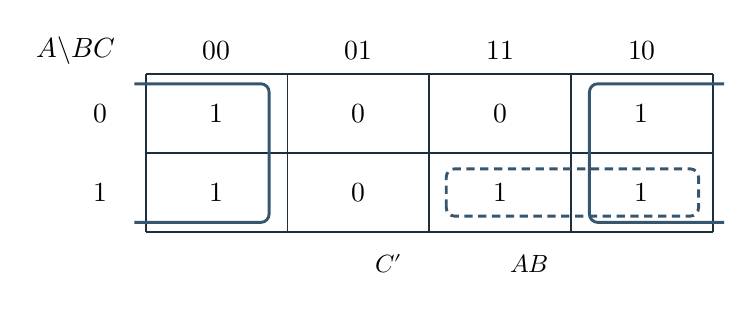
\begin{tikzpicture}[x=18mm,y=10mm,
 every node/.style={font=\normalsize},
 kgrid/.style={draw=ThemeMain!55!black,line width=0.65pt},
 kgroup/.style={draw=ThemeMain,line width=1.05pt,rounded corners=3pt}]
% Row and column headings are separated from the cells.
% Draw boundaries in the same coordinate system as the cell centres.
\foreach \x in {0,1,2,3,4}
 {\draw[kgrid] (\x,0)--(\x,2);}
\foreach \y in {0,1,2}
 {\draw[kgrid] (0,\y)--(4,\y);}
\foreach \s [count=\j from 0] in {00,01,11,10}
 {\node at (\j+.5,2.30){$\s$};}
\node at (-.50,2.30){$A\backslash BC$};
\node at (-.32,1.5){$0$};\node at (-.32,.5){$1$};
\foreach \v [count=\j from 0] in {1,0,0,1}
 {\node at (\j+.5,1.5){$\v$};}
\foreach \v [count=\j from 0] in {1,0,1,1}
 {\node at (\j+.5,.5){$\v$};}
% The open ends identify a single group across the map boundary.
\draw[kgroup] (-.08,.12)--(.87,.12)--(.87,1.88)--(-.08,1.88);
\draw[kgroup] (4.08,.12)--(3.13,.12)--(3.13,1.88)--(4.08,1.88);
% A dashed outline distinguishes the overlapping two-cell group.
\draw[kgroup,dash pattern=on 3pt off 2pt]
 (2.12,.20) rectangle (3.90,.80);
\node[font=\small,align=center] at (2,-.40)
 {实线：跨边界四格 $C'$\qquad 虚线：底行二格 $AB$};
\end{tikzpicture}
\end{center}
\endgroup
左右两端的四个 $1$ 组成跨边界圈，其中只有 $C=0$ 不变，得 $C'$；底行 $m_6,m_7$ 组成二格圈，得 $AB$。因此
\[
F=C'+AB.
\]
圈零时，$m_1,m_3$ 得和项 $A+C'$，$m_1,m_5$ 得 $B+C'$，故 $F=(A+C')(B+C')$。用第二分配律可验证两式等价。

\subsection{带无关项的化简与代码转换}
\begin{infobox}{例题：8421 BCD数码不小于5的判定}
输入 $ABCD$ 为有效8421 BCD码，$A$ 为最高位。数码不小于 $5$ 时输出 $F=1$。
\end{infobox}
\sol 成一编号为 $5,6,7,8,9$，无关编号为 $10$ 至 $15$。利用无关项得到 $F=A+BC+BD=A+B(C+D)$。有效输入中的 $4=0100$ 输出 $0$，$5=0101$ 输出 $1$。若输入允许全部四位二进制数，$10$ 至 $15$ 是否输出 $1$ 必须由新需求确定。

8421 BCD码 $WXYZ$ 转为余3码 $ABCD$ 时，每个输出分别化简，输入 $10$ 至 $15$ 作无关项，可取
\begin{align*}
A&=W+XY+XZ,\\
B&=X'Y+X'Z+XY'Z',\\
C&=YZ+Y'Z',\\
D&=Z'.
\end{align*}
这些公式仅承诺十个有效数码。也可用四位加法器执行 $WXYZ+0011$，但两种实现的非法输入行为未必相同。

\subsection{多变量图与代价判断}
五变量函数以 $A=0,1$ 分层时，可把两层对应的合法圈合并，消去 $A$；只出现在一层的圈须保留 $A$ 或 $A'$。若只分别化简两层再相加，可能遗漏跨层合并。

卡诺图适合少变量的手工化简。最简与或式和最简或与式以不同结构为目标，代价未必相同。多输出电路还可共享乘积项，逐输出独立最简未必给出整体最少门数。最后实现须考虑扇入、输出极性和延迟；无冒险实现也可能需要额外冗余项。

\subsection{四变量与五变量卡诺图例题}
\begin{infobox}{例题：十二个最小项的四变量化简}
2024秋期末回忆版，简答题3：求
\[
Y(A,B,C,D)=\sum m(0,1,2,3,4,6,8,9,10,11,12,14)
\]
的最简与或式，$A$ 为最高位。
\end{infobox}
\sol 行取 $AB$、列取 $CD$，均按 $00,01,11,10$ 排列。逐格按编号填写：
\begin{center}
\begin{tabular}{c|cccc}
\toprule $AB\backslash CD$&00&01&11&10\\\midrule
00&1&1&1&1\\
01&1&0&0&1\\
11&1&0&0&1\\
10&1&1&1&1\\\bottomrule
\end{tabular}
\end{center}
第一行与最后一行跨边界相邻，构成八格圈
\[
\{0,1,2,3,8,9,10,11\}\longrightarrow B'.
\]
其中 $A,C,D$ 均遍历 $0,1$，只有 $B=0$ 不变。第一列与最后一列也跨边界相邻，构成另一八格圈
\[
\{0,2,4,6,8,10,12,14\}\longrightarrow D'.
\]
两个圈允许重叠，且共同覆盖全部十二个 $1$，故
\[
Y=B'+D'.
\]
最简性可由零格判断：仅当 $B=D=1$ 时为零，故 $Y=(BD)'$。单个乘积项不能同时覆盖 $m_1$ 与 $m_4$ 而又避开零格 $m_5$，因此至少需要两项；所得两项均只有一个文字，不能再减少。

\begin{infobox}{例题：五变量图的跨层合并与孤立格}
课件03-3第38页：
\[
F(A,B,C,D,E)=\sum m(0,1,4,5,6,11,12,14,16,20,22,28,30,31).
\]
以 $A=0,1$ 分层，用卡诺图化简。$A,B,C,D,E$ 依次为编号从高到低的五位。
\end{infobox}
\sol 两层均以 $BC$ 为行、$DE$ 为列，按格雷顺序排列；右层编号比对应左层大 $16$。
\begin{center}
\begin{tabular}{c|cccc}
\toprule $A=0$&$DE=00$&01&11&10\\\midrule
$BC=00$&1&1&0&0\\
01&1&1&0&1\\
11&1&0&0&1\\
10&0&0&1&0\\\bottomrule
\end{tabular}\qquad
\begin{tabular}{c|cccc}
\toprule $A=1$&$DE=00$&01&11&10\\\midrule
$BC=00$&1&0&0&0\\
01&1&0&0&1\\
11&1&0&1&1\\
10&0&0&0&0\\\bottomrule
\end{tabular}
\end{center}
先找只能由一个最大圈覆盖的格，再把对应圈扩大。选取的圈与保留变量为
\begin{center}
\begin{tabularx}{\linewidth}{Y l Y}
\toprule 圈内编号 & 乘积项 & 消去的变量\\\midrule
$0,1,4,5$ & $A'B'D'$ & $C,E$ 遍历，保留 $A=B=D=0$\\
$0,4,16,20$ & $B'D'E'$ & 跨层消去 $A$，并消去 $C$\\
$4,6,12,14,20,22,28,30$ & $CE'$ & 两层对应四格合并；消去 $A,B,D$\\
$11$ & $A'BC'DE$ & 逻辑相邻的五格全为零，不能扩大\\
$30,31$ & $ABCD$ & 仅 $E$ 变化\\\bottomrule
\end{tabularx}
\end{center}
所以
\[
F=A'B'D'+B'D'E'+CE'+A'BC'DE+ABCD.
\]
格 $m_1,m_{16},m_6,m_{11},m_{31}$ 分别只能由表中对应最大圈覆盖，五项都不能省略。跨层合并须使用对应格；不能因为两层分别有 $1$ 就把不对应的格合为一圈。每一圈都只覆盖给定的成一编号，圈集的并集恰为题设集合。


\chapterpage{传播延迟、竞争与冒险}
\subsection{传播延迟与路径差异}
输入改变后，逻辑门输出需要一段时间才进入对应的稳定电平。\term{传播延迟} $t_{pLH}$ 表示输出低到高的延迟，$t_{pHL}$ 表示输出高到低的延迟；两者可不同，也受负载影响。多条信号路径汇合时，即使输入源同时改变，到达汇合点的时刻也可能不同。

\term{竞争}指多条路径的信号变化存在先后差异并可能产生相互影响；若输出因此出现逻辑上不应有的短脉冲或额外跳变，称为\term{冒险}或险象（hazard）。静态逻辑等价不保证瞬态波形等价。

\subsection{静态、动态与功能冒险}
\begin{center}
\begin{tabularx}{\linewidth}{l Y Y}
\toprule 类型 & 理想行为 & 可能的实际行为\\\midrule
静态1冒险 & 输出持续为1 & 短暂跌为0再回到1\\
静态0冒险 & 输出持续为0 & 短暂升为1再回到0\\
动态冒险 & 输出应只跳变一次 & 跳变多次后才稳定\\
功能冒险 & 多个输入由初值变为终值 & 中间输入组合造成错误输出\\\bottomrule
\end{tabularx}
\end{center}
静态和动态冒险常由单个输入变化沿不同路径传播引起；功能冒险涉及多个输入变化。发生冒险的实际脉冲宽度取决于路径延迟，逻辑分析通常判断“存在产生冒险的可能性”。

\begin{infobox}{例题：静态1冒险及冗余项}
两级与或电路 $F=AB+A'C$，当 $B=C=1$ 时，输入 $A$ 改变。
\end{infobox}
\sol 稳态逻辑为 $F=A+A'=1$。若原先导通的乘积项先变为 $0$，另一项尚未变为 $1$，输出可能出现低脉冲。加入共识项 $BC$：
\[
F_{\mathrm{safe}}=AB+A'C+BC.
\]
由共识定理，它与原函数稳态等价；$B=C=1$ 时，$BC$ 持续提供 $1$，覆盖两项交接的空隙。
\begin{center}
\begin{tikzpicture}[x=10mm,y=7mm]
\node[left] at (0,2.5){理想输出};\node[left] at (0,.5){有冒险输出};
\draw[ThemeMain,thick] (0,2.5)--(8,2.5);
\draw[ThemeMain,thick] (0,.5)--(3,.5)--(3,-.5)--(3.7,-.5)--(3.7,.5)--(8,.5);
\draw[->] (0,-1)--(8.5,-1) node[right] {$t$};
\draw[dashed,ThemeBorder] (3,3)--(3,-1);
\end{tikzpicture}
\end{center}

\subsection{代数判别与卡诺图判别}
代数判别可寻找在固定其他输入后变成 $X+X'$ 或 $XX'$ 的不同信号路径。仅看到某变量及其反变量出现，不足以直接断言有冒险，还须分析实现结构和固定条件。

对两级与或电路，若两个逻辑相邻的 $1$ 格没有被同一个乘积项圈共同覆盖，则单输入变化时存在静态1冒险的可能。补入跨越这两个格的圈，可消除该相邻转换的静态1冒险。对两级或与电路，同样检查相邻 $0$ 格是否被同一和项的零圈覆盖。
\[
F=(A+B)(A'+C)
\]
在 $B=C=0$ 时可能出现静态0冒险，加入和项 $B+C$ 得
\[
F_{\mathrm{safe}}=(A+B)(A'+C)(B+C).
\]
上述判据的前提是规定的两级结构、单输入变化和合法电平；不能据此保证任意多级电路或多输入跳变均无冒险。

\subsection{功能冒险与工程处理}
若 $F$ 在初值、终值上均为 $1$，但两个输入变化所经过的某个中间组合上为 $0$，真实电路可能出现功能冒险。例如 $F=A'BC+AB'+AC$，固定 $A=1$，输入 $BC$ 从 $00$ 变成 $11$：若 $B$ 先变，则经过 $10$，输出可能从 $1$ 跌为 $0$ 再回到 $1$；若 $C$ 先变，经过 $01$，输出保持 $1$。这种问题不能通过加入与原函数等价的冗余项改变规定成零组合的输出。

课件介绍增加冗余项、滤波电容和封锁/选通脉冲等方法。冗余项适于上述静态冒险；滤波属于电气处理，会改变负载与边沿，不能在逻辑模型中任意添加；选通信号应在电路充分稳定后采样。同步系统通常通过寄存器采样、时序约束和稳定的时钟使能控制避免把毛刺当作有效事件。组合译码信号直接用作时钟或异步清零时，对毛刺尤其敏感。

\subsection{由路径到达时间分析静态0冒险}
\begin{infobox}{例题：错误高脉冲的形成与消除}
依据课件03-4第7页的两级或与电路。设 $F=(A+B)(A'+C)$，$B=C=0$，$A$ 从 $0$ 变为 $1$。两和项 $p=A+B$、$q=A'+C$ 在末级与门输入处分别于 $3\,\mathrm{ns}$、$7\,\mathrm{ns}$ 完成变化；末级与门采用 $2\,\mathrm{ns}$ 的纯传输延迟模型。求输出可能出现的错误脉冲，并给出逻辑等价的消除办法。
\end{infobox}
\sol 稳态下 $p=A,q=A'$，故理想输出始终为 $AA'=0$。但传播途中，两个节点不是在同一时刻改变：
\begin{center}
\begin{tabular}{c c c c}
\toprule 时间区间 & $p$ & $q$ & 末级门的逻辑输入乘积 $pq$\\\midrule
$t<3\,\mathrm{ns}$&0&1&0\\
$3\le t<7\,\mathrm{ns}$&1&1&1\\
$t\ge7\,\mathrm{ns}$&1&0&0\\\bottomrule
\end{tabular}
\end{center}
中间四纳秒出现 $p=q=1$。按题定纯传输模型，两个跳变均延后 $2\,\mathrm{ns}$，因此 $F$ 在 $5\le t<9\,\mathrm{ns}$ 为 $1$，形成宽度 $4\,\mathrm{ns}$ 的错误高脉冲。这是静态0冒险。
\begin{center}
\begin{tikzpicture}[x=9mm,y=7mm,every node/.style={font=\small}]
\foreach \y/\lab in {4/p,2/q,0/F}
 {\node[left] at (0,\y+.4){$\lab$};}
\draw[ThemeMain,thick] (0,4)--(3,4)--(3,5)--(10,5);
\draw[ThemeMain,thick] (0,3)--(7,3)--(7,2)--(10,2);
\draw[ThemeMain,thick] (0,0)--(5,0)--(5,1)--(9,1)--(9,0)--(10,0);
\draw[->] (0,-.6)--(10.6,-.6) node[right] {$t/\mathrm{ns}$};
\foreach \t in {0,3,5,7,9}
 {\draw (\t,-.55)--(\t,-.7);\node[below] at (\t,-.7){$\t$};}
\end{tikzpicture}
\end{center}
或与结构可加入冗余和项 $B+C$：
\[
F_{\mathrm{safe}}=(A+B)(A'+C)(B+C).
\]
依据共识定理的对偶式，加入该项不改变稳定逻辑功能。当 $B=C=0$ 时，这个和项持续为零，使末级输出保持零，不再依靠两条 $A$ 路径恰好同时切换。实际门可能具有惯性延迟，短脉冲是否传播还取决于器件；本题的脉冲时刻仅适用于给定的纯传输模型。


\chapterpage{组合逻辑电路的分析与设计}
\subsection{分析步骤与设计步骤}
组合电路分析从已知电路出发：为中间节点命名，逐级写表达式，代入得到输出函数，化简并列真值表，最后说明实际功能。设计从需求出发，方向相反。
\begin{infobox}{方法：组合逻辑设计的完整步骤}
\begin{enumerate}
\item 规定输入、输出的意义、位宽、有效电平和合法输入集合。
\item 把需求写成真值表；只有确定不使用的组合才标无关项。
\item 写标准表达式或填写卡诺图，按所需结构化简。
\item 按门类型、扇入、输出极性与共享项转换实现形式，画逻辑图或编写 HDL。
\item 核对全部合法组合，再检查延迟、冒险、使能和负载条件。
\end{enumerate}
\end{infobox}
规模、速度、功耗、价格和可靠性可能相互制约。不同实现可具有相同真值表而物理性能不同。

\subsection{表决器、裁判电路与操作码形成器}
三人多数表决输出为 $F=AB+AC+BC$。若主裁判 $A$ 与副裁判 $B,C$ 按课件规则控制红、绿灯，红灯为 $R$、绿灯为 $G$，则
\[
R=A+BC,\qquad G=A(B+C).
\]
主裁判单独同意，或只有两名副裁判同意时，$R=1,G=0$；主裁判与至少一名副裁判同意时，两灯均亮。其余情况两灯均灭，且 $G=1$ 必然有 $R=1$。

操作码形成器设 $A,B,C$ 分别为乘、加、减键，只有单键按下才有效；约定无键按下输出 $00$，乘、加、减输出分别为 $01,10,11$。以 $F_2F_1$ 为输出，得到
\[
F_2=B+C,\qquad F_1=A+C.
\]
若规定同时按键必须输出错误标志，不能继续把多键组合当作无关项，须另设有效性输出或重新定义操作码。

\subsection{多输出函数：两位数的平方}
\begin{infobox}{例题：平方电路}
无符号两位输入 $X=x_1x_0$，四位输出 $Y=y_3y_2y_1y_0=X^2$。
\end{infobox}
\sol $X=0,1,2,3$ 时输出分别为 $0000,0001,0100,1001$，逐列得到
\[
y_3=x_1x_0,\qquad y_2=x_1x_0',\qquad y_1=0,\qquad y_0=x_0.
\]
这里 $y_2$ 必须包含 $x_0'$，因为 $X=3$ 的平方为 $9$，其 $2^2$ 位为 $0$。多输出设计应分别核对每一列，而非由某个输出的化简结果推测其他输出。

\subsection{半加器、全加器与进位}
\term{半加器}相加两个一位数 $a_i,b_i$，输出本位和 $S_i$ 与进位 $C_i$：
\[
S_i=a_i\oplus b_i,\qquad C_i=a_ib_i.
\]
\term{全加器}还接受来自低位的进位 $C_{i-1}$。根据三个一位输入的算术和，和位是奇偶性，进位是多数函数：
\begin{infobox}{公式：全加器}
\[
S_i=a_i\oplus b_i\oplus C_{i-1},
\]
\[
C_i=a_ib_i+(a_i\oplus b_i)C_{i-1}
=a_ib_i+a_iC_{i-1}+b_iC_{i-1}.
\]
$C_{-1}$ 表示最低位的外部输入进位，与课件编号一致。
\end{infobox}
\begin{center}
\begin{tabular}{ccc cc}
\toprule $a_i$&$b_i$&$C_{i-1}$&$S_i$&$C_i$\\\midrule
0&0&0&0&0\\0&0&1&1&0\\0&1&0&1&0\\0&1&1&0&1\\
1&0&0&1&0\\1&0&1&0&1\\1&1&0&0&1\\1&1&1&1&1\\\bottomrule
\end{tabular}
\end{center}
四位数 $1011+1110$ 的五位结果为 $11001$；最低位和到最高位和构成 $1001$，末级进位为 $1$。输出宽度若只有四位，最高进位会被截去。

多个全加器\term{串行进位}时，高位必须等待低位进位，最坏延迟随位数线性增长。设\term{进位传递} $P_i=a_i\oplus b_i$、\term{进位产生} $G_i=a_ib_i$，则 $C_i=G_i+P_iC_{i-1}$。逐层展开得
\begin{align*}
C_0&=G_0+P_0C_{-1},\\
C_1&=G_1+P_1G_0+P_1P_0C_{-1},\\
C_2&=G_2+P_2G_1+P_2P_1G_0+P_2P_1P_0C_{-1},\\
C_3&=G_3+P_3G_2+P_3P_2G_1+P_3P_2P_1G_0\\
&\quad+P_3P_2P_1P_0C_{-1}.
\end{align*}
\term{超前进位}利用输入直接并行生成进位，以更多组合逻辑减少逐位等待。大位宽实现常分组处理，不能假设任意长乘积项可由无延迟、无限扇入的门实现。课件采用异或定义 $P_i$，有些资料采用 $a_i+b_i$；两种进位约定不能未经说明混用和位公式。

\subsection{全减器与借位}
全减器计算 $a_i-b_i-B_{i-1}$，$B_{i-1}$ 为低位借入，输出差位 $D_i$ 与向高位的借位 $B_i$。用 $B_i$ 区别于加法进位：
\[
D_i=a_i\oplus b_i\oplus B_{i-1},\qquad
B_i=a_i'b_i+a_i'B_{i-1}+b_iB_{i-1}.
\]
当 $a_i=0$ 时，只要 $b_i$ 或借入为 $1$ 就须借位；当 $a_i=1$ 时，只有二者均为 $1$ 才须借位。这也得到
\[
B_i=a_i'(b_i\oplus B_{i-1})+b_iB_{i-1}.
\]
$1110_2-1011_2=0011_2$，最终借位为零。加法与减法的和位、差位均为三输入异或，但进位与借位函数不同。

\subsection{三态门与总线}
\term{三态缓冲器}在输出 $0,1$ 以外，还可输出\term{高阻态} $Z$。高电平使能 $E$ 的非反相缓冲器在 $E=1$ 时输出输入 $A$，在 $E=0$ 时输出 $Z$。高阻近似电气断开，不是第三种普通布尔真值。

多个输出通过三态门连接同一总线时，任一时刻通常只能有一个驱动器有效。两个有效驱动器分别输出 $0,1$ 会造成总线争用；所有驱动器禁用时，总线不等于自动输出零，是否有确定电平取决于上拉、下拉或保持电路。双向总线的方向与使能应共同控制。

\begin{infobox}{例题：选择能被5整除的BCD数码}
输入 $X=x_3x_2x_1x_0$ 为8421 BCD码，只有数码 $0,5$ 时允许其数据驱动输出总线。
\end{infobox}
\sol 使能函数的成一编号为 $0,5$，无关编号为 $10$ 至 $15$，可取
\[
E=x_2x_1'x_0+x_3'x_2'x_1'x_0'.
\]
各数据位通过共同受 $E$ 控制的三态门传送。$E=0$ 时输出为高阻，而非四位零码；零数码被选中时则主动输出 $0000$。这两种状态必须区分。

\subsection{从门电路逐级求函数}
\begin{infobox}{例题：四个或非门组成的比较电路}
2024秋期末回忆版，简答题6。分析下图，写出 $Y_1,Y_2,Y_3$ 的最简与或式及逻辑功能。输入 $A,B$ 均为一位无符号数。
\end{infobox}
\begin{center}
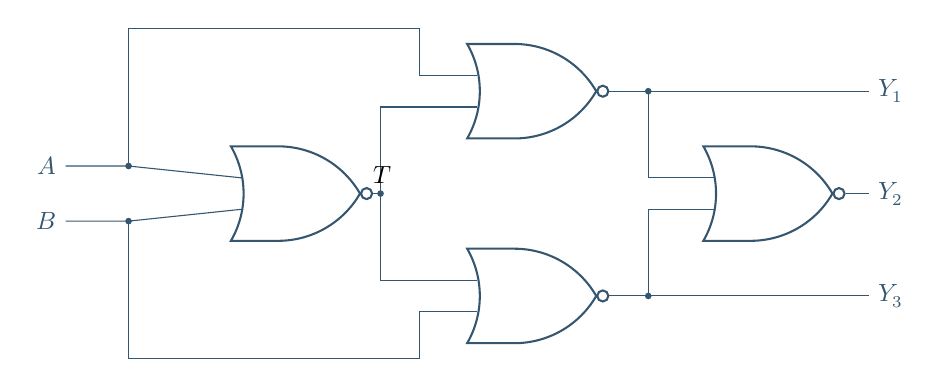
\begin{tikzpicture}[every node/.style={font=\small},
 ng/.style={nor gate US,draw=ThemeMain,line width=.75pt,
 logic gate inputs=nn,minimum width=15mm,minimum height=12mm}]
\node[ng] (g0) at (2,0) {};
\node[ng] (g1) at (5,1.3) {};
\node[ng] (g3) at (5,-1.3) {};
\node[ng] (g2) at (8,0) {};
\coordinate (a) at (0,.35);\coordinate (b) at (0,-.35);
\draw[ThemeMain] (-.8,.35) node[left]{$A$}--(a)--(g0.input 1);
\draw[ThemeMain] (-.8,-.35) node[left]{$B$}--(b)--(g0.input 2);
\draw[ThemeMain] (a)--(0,2.1)--(3.7,2.1)|-(g1.input 1);
\draw[ThemeMain] (b)--(0,-2.1)--(3.7,-2.1)|-(g3.input 2);
\draw[ThemeMain] (g0.output)--(3.2,0) coordinate (t);
\draw[ThemeMain] (t)|-(g1.input 2);
\draw[ThemeMain] (t)|-(g3.input 1);
\node[above] at (3.2,0){$T$};
\draw[ThemeMain] (g1.output)--(6.6,1.3) coordinate (y1)--(9.4,1.3) node[right]{$Y_1$};
\draw[ThemeMain] (g3.output)--(6.6,-1.3) coordinate (y3)--(9.4,-1.3) node[right]{$Y_3$};
\draw[ThemeMain] (y1)|-(g2.input 1);
\draw[ThemeMain] (y3)|-(g2.input 2);
\draw[ThemeMain] (g2.output)--(9.4,0) node[right]{$Y_2$};
\foreach \p in {a,b,t,y1,y3}\fill[ThemeMain] (\p) circle (1.2pt);
\end{tikzpicture}
\end{center}
\sol 门输出端的小圆圈表示取反。先给第一级输出命名 $T$，再写后级函数；导线分支上的实心点表示电气连接。
\begin{align*}
T&=(A+B)',\\
Y_1&=(A+T)'=A'T'=A'(A+B)=A'B,\\
Y_3&=(B+T)'=B'T'=B'(A+B)=AB',\\
Y_2&=(Y_1+Y_3)'=(A'B+AB')'=AB+A'B'.
\end{align*}
最后一式可由异或取反得到，也可按德摩根律展开后吸收。列出真值表核对输出的含义：
\begin{center}
\begin{tabular}{cc ccc l}
\toprule $A$&$B$&$Y_1$&$Y_2$&$Y_3$&比较结果\\\midrule
0&0&0&1&0&相等\\0&1&1&0&0&$A<B$\\
1&0&0&0&1&$A>B$\\1&1&0&1&0&相等\\\bottomrule
\end{tabular}
\end{center}
这是一个一位数值比较器：$Y_1$ 指示小于，$Y_2$ 指示相等，$Y_3$ 指示大于，稳定时三者恰有一个为 $1$。若只看门的数量或图形外观，无法判断功能；须从连接关系求出函数。反相小圆圈属于门符号，不能当作导线上的分支连接点。

\subsection{文字条件到控制电路的设计}
\begin{infobox}{例题：缆车启动条件}
2024秋期末回忆版，设计题1。两辆缆车的方向分别为 $A,B$：$1$ 表示上行，$0$ 表示下行。门状态为 $C$：$1$ 表示关闭。要求两车一上一下且门关闭才允许启动，输出 $Y=1$ 表示允许。求函数并画逻辑图。
\end{infobox}
\sol “一上一下”只对应 $AB=01$ 或 $10$，不是“至少一车上行”。再与关门条件相与，得到
\[
Y=(A'B+AB')C=A'BC+AB'C=(A\oplus B)C.
\]
按全部八种组合列表，成一编号仅为 $3,5$：
\begin{center}
\begin{tabular}{ccc c l}
\toprule $A$&$B$&$C$&$Y$&不允许时的原因\\\midrule
0&0&0&0&方向相同且门开\\0&0&1&0&方向相同\\
0&1&0&0&门开\\0&1&1&1&满足全部条件\\
1&0&0&0&门开\\1&0&1&1&满足全部条件\\
1&1&0&0&方向相同且门开\\1&1&1&0&方向相同\\\bottomrule
\end{tabular}
\end{center}
用一个异或门判断方向不同，再用与门加入关门条件：
\begin{center}
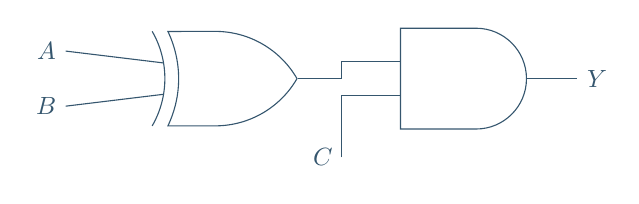
\begin{tikzpicture}[every node/.style={font=\small}]
\node[xor gate US,draw=ThemeMain,logic gate inputs=nn,
 minimum width=16mm,minimum height=12mm] (x) at (2,0) {};
\node[and gate US,draw=ThemeMain,logic gate inputs=nn,
 minimum width=16mm,minimum height=12mm] (g) at (5,0) {};
\draw[ThemeMain] (0,.35) node[left]{$A$}--(x.input 1);
\draw[ThemeMain] (0,-.35) node[left]{$B$}--(x.input 2);
\draw[ThemeMain] (x.output)--(3.5,0)|-(g.input 1);
\draw[ThemeMain] (3.5,-1) node[left]{$C$}|-(g.input 2);
\draw[ThemeMain] (g.output)--(6.5,0) node[right]{$Y$};
\end{tikzpicture}
\end{center}
若仅允许与、或、非门，就把异或展开为 $A'B+AB'$，再与 $C$ 相与。验算 $AB=11,C=1$ 必须输出零；误写为 $(A+B)C$ 会在这一组合错误地允许启动。本题实现逻辑条件；实际设备还须由完整控制系统处理故障与执行过程，题目未要求状态存储。


\chapterpage{常用组合逻辑器件与可编程逻辑}
\subsection{二进制译码器及使能极性}
\term{二进制译码器}将 $n$ 位代码转换为 $2^n$ 条选择线，启用时只有一条有效，每一条对应一个最小项。输出高电平有效时 $Y_i=m_i$；低电平有效时输出引脚电平 $y_i=m_i'=M_i$。

74LS138 为三线—八线译码器，地址输入 $CBA$ 中 $C$ 为最高位、$A$ 为最低位。它要求 $G_1=1$、$G_{2A}=G_{2B}=0$ 才启用；启用时被选中的输出为 $0$、其余为 $1$，禁用时全部输出为 $1$。这里 $G_{2A},G_{2B}$ 指引脚电平，即使器件图上的名称带横线，仍须按低电平有效读表。该极性依据\href{https://www.ti.com/lit/ds/symlink/sn74ls138.pdf}{TI 74LS138数据手册}核对。

\begin{infobox}{例题：译码器实现全加器}
把全加器输入 $a,b,c$ 分别接到74LS138的 $C,B,A$，并使器件启用。
\end{infobox}
\sol 和位 $S=\sum m(1,2,4,7)$，进位 $C_{\mathrm{out}}=\sum m(3,5,6,7)$。由于 $y_i=m_i'$，用与非门合成
\[
S=(y_1y_2y_4y_7)',\qquad C_{\mathrm{out}}=(y_3y_5y_6y_7)'.
\]
全减器的差位同样使用 $1,2,4,7$，借位使用 $1,2,3,7$。低有效输出不能直接用普通或门合成成一最小项。

\subsection{译码扩展与地址译码}
两片74LS138共用低三位地址 $CBA$，第四位 $D$ 分别启用低组、高组，可构成四线—十六线译码器。令低组 $G_1=1,G_{2A}=D,G_{2B}=0$；高组 $G_1=D,G_{2A}=G_{2B}=0$。$D=0$ 时只有低组启用，$D=1$ 时只有高组启用。

\term{地址译码}用高位地址确定片选，低位地址确定器件内部单元。未参加片选比较的地址位能自由变化；若本应参与的高位被遗漏，会出现地址镜像。
\begin{infobox}{例题：16位地址空间分配}
八个存储芯片各有13位内部地址，以 $A_{15}A_{14}A_{13}$ 译码选择芯片。求第 $k$ 片（$k=0,\ldots,7$）的地址范围。
\end{infobox}
\sol 每片有 $2^{13}=8192$ 个地址，范围为
\[
[k\cdot2^{13},(k+1)2^{13}-1].
\]
从第一片到第八片依次为 $0000$--$1FFF$、$2000$--$3FFF$、$4000$--$5FFF$、$6000$--$7FFF$、$8000$--$9FFF$、$A000$--$BFFF$、$C000$--$DFFF$、$E000$--$FFFF$（均为十六进制）。

若使能固定 $A_{15}\cdots A_{12}=0001$，$CBA=A_{11}A_{10}A_9$，低九位自由，则整体范围为 $1000$--$1FFF$；选择编号 $2$ 的外设范围为 $1400$--$15FF$。求范围须从实际连线读出所有固定条件，不能只数地址线。

\subsection{显示译码与七段数码管}
\term{显示译码器}把输入代码转换为点亮字形所需的段选信号。七段从顶部开始依次标为 $a$（上）、$b$（右上）、$c$（右下）、$d$（下）、$e$（左下）、$f$（左上）、$g$（中）。共阴极通常高电平点亮，共阳极通常低电平点亮；还需限流及合适驱动能力。
\begin{center}
\begin{tabular}{c c c c c c c c}
\toprule 数码 & $a$&$b$&$c$&$d$&$e$&$f$&$g$\\\midrule
0&1&1&1&1&1&1&0\\1&0&1&1&0&0&0&0\\2&1&1&0&1&1&0&1\\
3&1&1&1&1&0&0&1\\4&0&1&1&0&0&1&1\\5&1&0&1&1&0&1&1\\
6&1&0&1&1&1&1&1\\7&1&1&1&0&0&0&0\\8&1&1&1&1&1&1&1\\9&1&1&1&1&0&1&1\\\bottomrule
\end{tabular}
\end{center}
上表为常用共阴极字形，$1$ 表示点亮。设 $ABCD$ 是8421 BCD输入，利用非法码作无关项，前三段可取
\[
a=A+C+BD+B'D',\quad b=B'+CD+C'D',\quad c=B+C'+D.
\]
其他段按对应列分别化简。若非法输入须熄灭，必须把相应输出指定为零，而不能继续作无关项。

\subsection{多路选择器与函数实现}
\term{多路选择器}（MUX，也称多路复用器、数据选择器）按 $n$ 位选择信号，在 $2^n$ 路数据中选一路输出。启用时
\[
Y=\sum_{k=0}^{2^n-1}m_k(\symbf{S})I_k.
\]
$\symbf{S}$ 是选择向量，$m_k$ 是其最小项，$I_k$ 是第 $k$ 路输入。二选一为 $Y=S'I_0+SI_1$，可直接实现香农展开。

若函数输入数等于选择位数，数据端按真值表接 $0,1$；若输入数少于选择位数，剩余选择端接确定常量，并按实际编号接数据；若输入数多于选择位数，数据端接剩余输入的余因子。
\begin{infobox}{例题：四选一实现三人多数函数}
选择端取 $AB$，用四选一MUX实现 $F=AB+AC+BC$。
\end{infobox}
\sol 固定 $AB$，依次得到 $I_0=0,I_1=C,I_2=C,I_3=1$。这比八选一直接接八个常量少用一个选择输入。

四变量函数降成三变量图时，每格是关于余下变量 $D$ 的函数。若 $F|_{D=0},F|_{D=1}$ 分别为 $0,0$、$0,1$、$1,0$、$1,1$，该数据端分别接 $0,D,D',1$。再少一个选择位时，数据端须实现两变量余因子，而非只能接上述四种值。

74LS151为八选一，低有效选通端 $G=0$ 时，同相输出 $Y=I_k$，反相输出 $W=I_k'$；$G=1$ 时 $Y=0,W=1$，两者均不是高阻。这依据\href{https://www.ti.com/lit/ds/symlink/sn74ls151.pdf}{TI 74LS151数据手册}。74LS153包含两个四选一单元，公共选择端、独立低有效使能，禁用输出为零。

扩展为三十二选一的一种直接方案是四个八选一作为第一级，共用低三位选择，再用一个四选一按高两位选其输出。也可用译码器分别使能四片74LS151，但须按禁用输出极性添加汇合门：同相输出可用或门汇合，不能直接把推挽输出短接。

\term{多路分配器}（DEMUX）把一路数据送到选择的一个输出，其余输出为规定的非有效值。高有效结构可写 $Y_k=m_k(\symbf S)D$。MUX控制数据源，DEMUX控制数据目的地；译码器提供选择条件。

\subsection{普通编码器、优先编码器与有效标志}
\term{普通编码器}在 $2^n$ 路输入中仅一路有效的前提下，输出该路的 $n$ 位编号。四线—二线高有效编码器的输出为 $B_1=I_2+I_3,B_0=I_1+I_3$。多个输入同时有效时，这两式不再保证正确对象编号。

\term{优先编码器}允许多路请求同时有效，按指定优先级输出最高优先级的编号。若 $I_3>I_2>I_1>I_0$，可取
\[
B_1=I_3+I_2,\qquad B_0=I_3+I_2'I_1,\qquad
V=I_3+I_2+I_1+I_0.
\]
$V$ 是有效标志，区分“没有请求”和“第0路有效”；二者的编号都可能是 $00$。

课件的低有效十进制键盘以 $P_1,\ldots,P_9$ 表示按键线，最多一键有效，零键或无键均编为 $0000$。对应8421码输出为
\begin{align*}
W&=(P_8P_9)',&X&=(P_4P_5P_6P_7)',\\
Y&=(P_2P_3P_6P_7)',&Z&=(P_1P_3P_5P_7P_9)'.
\end{align*}
若须区分数字零与无键，应另设按键有效信号。优先编码器记录的是优先规则，不会自动记录哪个按键最先到达；抢答功能还需状态存储。

\subsection{奇偶校验}
设数据位为 $A_{n-1},\ldots,A_0$，异或和为 $P=\bigoplus_i A_i$。\term{偶校验}使包括校验位在内的总 $1$ 数为偶数，故校验位 $P_E=P$；\term{奇校验}使总 $1$ 数为奇数，故 $P_O=P'$。
\begin{infobox}{公式：接收端检测}
包括校验位的接收字为 $R_n\cdots R_0$。偶校验错误标志为 $E_E=\bigoplus_{i=0}^{n}R_i$；奇校验错误标志为 $E_O=(\bigoplus_{i=0}^{n}R_i)'$。标志为 $1$ 表示不满足约定的奇偶性。
\end{infobox}
任意奇数位翻转都会改变奇偶性，任意偶数位翻转不会改变奇偶性。因此校验通过仅表示没有发现奇偶性错误，不能断言没有传输错误；奇偶校验不能定位错误或纠正错误。

74LS280有九个输入，输出 ODD 在输入含奇数个 $1$ 时为 $1$，EVEN 则是其反。用它生成八位数据的奇校验位，可把第九输入接 $0$，取 EVEN；检测时九位输入为数据与奇校验位，取 EVEN 作为错误标志。示例数据 $10110010$ 含四个 $1$，偶校验位为 $0$，奇校验位为 $1$。

\subsection{数值比较器及级联}
一位比较器有三个互斥输出：相等 $E=A\odot B$、大于 $G=AB'$、小于 $L=A'B$。无符号多位数从高位开始比较，只有高位相等才比较低位。

令第 $i$ 位 $e_i=a_i\odot b_i$、$g_i=a_ib_i'$、$l_i=a_i'b_i$。四位比较为
\begin{align*}
E&=e_3e_2e_1e_0,\\
G&=g_3+e_3g_2+e_3e_2g_1+e_3e_2e_1g_0,\\
L&=l_3+e_3l_2+e_3e_2l_1+e_3e_2e_1l_0.
\end{align*}
74LS85的级联输入传入低位组的比较结果；独立比较一组时按“相等、大于、小于”的顺序置为 $1,0,0$。串行级联把低位输出传到高位输入，最高组产生总结果。

并行分组时，各组先独立比较，再由组间逻辑从高组向低组决定结果。以四组为例，将 $e_i,g_i,l_i$ 换为每组的结果，仍用上述形式。课件的64位实现把八组8位的 GT、LT标志组成两个8位向量，再比较这两个向量：最高一个不相等的组在 GT、LT中分别为 $10$ 或 $01$，故第二级比较正确判定全字大小；若全部组相等，两向量均为零。该方法依赖组输出互斥及组序正确，不能把任意标志向量如此比较。

逻辑规模随位数增长；串行优先链的深度随位数或组数线性增加，树形分层可降低逻辑深度。比较有符号数时，必须使用相应的有符号解释，不能套用无符号高位比较规则。

\subsection{ROM、乘积项阵列与FPGA查找表}
\term{只读存储器}（ROM）在固定内容、异步读模型中可看作一个 $n$ 输入、$b$ 输出的组合逻辑：输入是地址，存储的每一行是该地址的输出。组织为 $2^n\times b$，总容量为 $2^nb$ 位。实际同步读存储器可能带输出寄存器，不能一概视为纯组合电路。
\begin{infobox}{例题：ROM实现四位乘四位无符号乘法}
两个四位数 $X,Y$ 输入，ROM输出乘积。
\end{infobox}
\sol 地址可取 $\{X,Y\}$，共八位、$256$ 种组合。最大乘积 $15\times15=225=(11100001)_2$，需要八位输出，故用 $256\times8$ ROM，容量 $2048$ 位。每个地址存放对应乘积。程序可生成表内容，再用独立算术结果核对。

输出极性可控的二线—四线译码器有两个地址输入和一个极性控制输入，共三位；输出四位，故可用 $8\times4$ ROM。高有效与低有效两套译码表各占四行。

在乘积项结构中，PROM常对应固定与阵列、可编程或阵列；PLA的与、或阵列均可编程；PAL通常与阵列可编程、或阵列固定；GAL可再编程并提供可配置宏单元。CPLD通常组合多个逻辑块与互连，具体实现依器件而定。

\term{查找表}（LUT）对 $k$ 个输入存储 $2^k$ 个输出真值，可实现任意 $k$ 输入的一位布尔函数。四输入与门的16个表项只有地址 $1111$ 对应 $1$，其余为 $0$。LUT表内容可由配置存储位保存，不能把所有FPGA一概描述为同一种存储技术。

FPGA含 LUT、触发器、选择器、进位链与可编程互连，还可能含块存储、DSP、输入输出块和时钟网络。可配置逻辑块CLB及slice的具体构成依器件系列而定；课件中的7系列例子说明一种架构，不是所有FPGA的统一规格。实现功能仍受资源数量、接口和时序限制。

\subsection{复杂使能条件的地址译码}
\begin{infobox}{例题：由使能门与译码编号求地址范围}
2024秋期末回忆版，简答题4。地址为 $A_{15}\cdots A_0$，外设内部接低八位 $A_7\cdots A_0$。电路连接见图：$G_1=(A_{14}+A_{12})'$，$G_{2A}=A_{13}$，$G_{2B}=(A_{15}A_{11})'$；设备1接低有效输出 $Y_3$。题面明确规定译码器 $A$ 端为高位、$C$ 端为低位。求全地址译码范围及设备1范围，并与通常74LS138编号约定比较。
\end{infobox}
\begin{center}
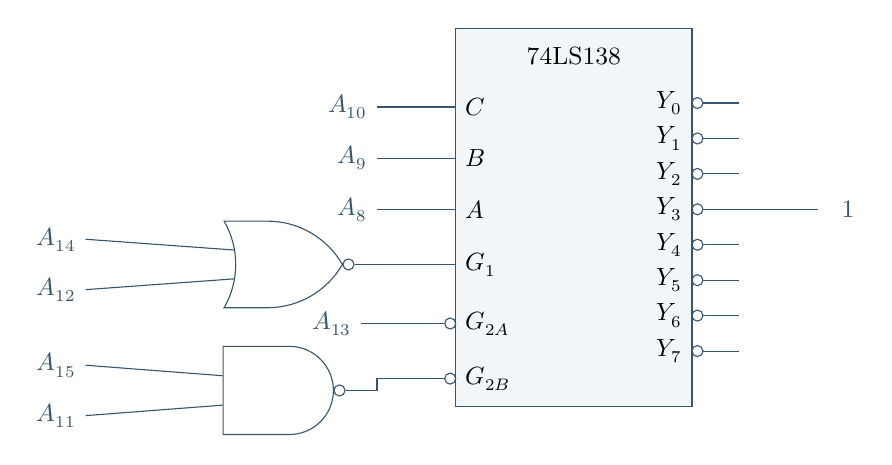
\begin{tikzpicture}[every node/.style={font=\small}]
\draw[ThemeMain,fill=ThemeBack] (5,0) rectangle (8,4.8);
\node at (6.5,4.45){74LS138};
\foreach \y/\lab/\in in {3.8/C/A_{10},3.15/B/A_9,2.5/A/A_8}
 {\node[right] at (5,\y){$\lab$};\draw[ThemeMain] (4,\y) node[left]{$\in$}--(5,\y);}
\node[right] at (5,1.8){$G_1$};
\node[right] at (5,1.05){$G_{2A}$};
\node[right] at (5,.35){$G_{2B}$};
\node[nor gate US,draw=ThemeMain,logic gate inputs=nn,
 minimum width=14mm,minimum height=11mm] (or) at (2.7,1.8) {};
\node[nand gate US,draw=ThemeMain,logic gate inputs=nn,
 minimum width=14mm,minimum height=11mm] (and) at (2.7,.2) {};
\draw[ThemeMain] (.3,2.12) node[left]{$A_{14}$}--(or.input 1);
\draw[ThemeMain] (.3,1.48) node[left]{$A_{12}$}--(or.input 2);
\draw[ThemeMain] (or.output)--(5,1.8);
\draw[ThemeMain] (3.8,1.05) node[left]{$A_{13}$}--(4.86,1.05);
\draw[ThemeMain] (4.93,1.05) circle (.07);
\draw[ThemeMain] (.3,.52) node[left]{$A_{15}$}--(and.input 1);
\draw[ThemeMain] (.3,-.12) node[left]{$A_{11}$}--(and.input 2);
\draw[ThemeMain] (and.output)--(4,.2)|-(4.86,.35);
\draw[ThemeMain] (4.93,.35) circle (.07);
\foreach \i in {0,...,7}{
 \pgfmathsetmacro{\yy}{3.85-.45*\i}
 \node[left] at (8,\yy){$Y_{\i}$};
 \draw[ThemeMain] (8.07,\yy) circle (.07);
 \draw[ThemeMain] (8.14,\yy)--(8.6,\yy);
}
\draw[ThemeMain] (8.6,2.5)--(9.6,2.5) node[right]{设备1};
\end{tikzpicture}
\end{center}
\sol 先求启用条件。$G_1=1$ 要求 $A_{14}=A_{12}=0$；两个低有效使能输入必须为零，故 $A_{13}=0$ 且 $A_{15}=A_{11}=1$。所以
\[
A_{15}A_{14}A_{13}A_{12}A_{11}=10001.
\]
剩余 $A_{10}\cdots A_0$ 全可变化，整个电路的连续地址范围为
\[
1000\,1000\,0000\,0000_2\ \text{至}\ 1000\,1111\,1111\,1111_2
\quad\Longrightarrow\quad \mathrm{8800\!\sim\!8FFF}_{16}.
\]
按本题文字规定，译码编号的三位是 $ABC=A_8A_9A_{10}$。$Y_3$ 选中时 $A_8A_9A_{10}=011$，地址字中的实际高到低顺序则为 $A_{10}A_9A_8=110$。设备1因此占
\[
\mathrm{8E00\!\sim\!8EFF}_{16},\qquad 2^8=256\text{ 个地址}.
\]
通常74LS138数据手册及本讲义前文按 $CBA$ 编号，$A$ 为最低位。若按真实器件约定，$Y_3$ 要求 $A_{10}A_9A_8=011$，设备范围改为 $\mathrm{8B00\!\sim\!8BFF}_{16}$，整体范围仍为 $\mathrm{8800\!\sim\!8FFF}_{16}$。回忆版题面与通常约定存在冲突，应先注明采用哪一个约定，不能混用两者得出唯一答案。

\subsection{数据选择、优先编码与校验的完整计算}
\begin{infobox}{例题：八选一实现四变量函数}
按课件04-2的数据选择器方法改编。用一个启用的八选一MUX实现
\[
F(A,B,C,D)=\sum m(0,1,2,5,7,8,9,10,12,14),
\]
取 $ABC$ 为从高到低的选择字，求全部数据端 $I_0$ 至 $I_7$ 的连接。
\end{infobox}
\sol 固定 $ABC=k$，分别检查编号 $2k$、$2k+1$ 是否在成一集合中，即得到 $D=0,1$ 时的两个输出。再按 $00\to0,01\to D,10\to D',11\to1$ 翻译为余因子：
\begin{center}
\begin{tabular}{c c cc c}
\toprule $ABC$&最小项编号&$D=0$&$D=1$&数据端\\\midrule
000&$0,1$&1&1&$I_0=1$\\
001&$2,3$&1&0&$I_1=D'$\\
010&$4,5$&0&1&$I_2=D$\\
011&$6,7$&0&1&$I_3=D$\\
100&$8,9$&1&1&$I_4=1$\\
101&$10,11$&1&0&$I_5=D'$\\
110&$12,13$&1&0&$I_6=D'$\\
111&$14,15$&1&0&$I_7=D'$\\\bottomrule
\end{tabular}
\end{center}
只须一个反相器提供 $D'$。若使用74LS151，逻辑选择字 $ABC$ 须按本讲义前文的器件位序接入：器件 $C,B,A$ 端分别接函数变量 $A,B,C$，使能端接低电平，取同相输出。输入 $ABCD=1101$ 选 $I_6=D'=0$，与编号13不在成一集合中一致；不能按函数变量字母直接接同名字引脚而忽略位权。

\begin{infobox}{例题：同时有效的请求与编码有效标志}
按课件04-2的优先编码方法改编。八路高有效请求 $I_7\cdots I_0$，下标越大优先级越高，输出编号 $B_2B_1B_0$ 和有效标志 $V$。求请求字 $01001000$ 的输出，并解释为什么普通编码器不适用。
\end{infobox}
\sol 请求字中 $I_6=I_3=1$，应只编码第6路。为逐层屏蔽低优先级请求，定义
\[
H_7=I_7,\qquad H_k=I_k\prod_{j=k+1}^{7}I_j'\quad(0\le k<7).
\]
$H_k=1$ 表示第 $k$ 路为本次获选请求，至多一个 $H_k$ 为 $1$。输出为
\begin{align*}
B_2&=H_4+H_5+H_6+H_7,\\
B_1&=H_2+H_3+H_6+H_7,\\
B_0&=H_1+H_3+H_5+H_7,\qquad V=\sum_{k=0}^{7}I_k.
\end{align*}
本题 $H_6=1$，而 $H_3$ 的乘积中含 $I_6'=0$，所以 $H_3=0$，得到 $(B_2B_1B_0,V)=(110,1)$。若把普通编码器的输出直接写成对应请求的或，$I_6$ 与 $I_3$ 同时有效会得到错误的 $111$，表示根本没有请求的第7路。

边界情况也须区分：仅 $I_0=1$ 时输出 $(000,1)$；没有请求时规定输出 $(000,0)$。编号零不等于没有请求，因此有效标志不能省略。低有效芯片须按其功能表转换极性，不能直接照搬本题高有效式。

\begin{infobox}{例题：奇偶校验的生成、检验与漏检}
按课件04-2的奇偶校验方法改编。八位数据为 $11010010$，求偶校验位和奇校验位；以偶校验传输为例，比较一个数据位翻转与两个数据位翻转。
\end{infobox}
\sol 数据中有四个 $1$，异或和为 $P=0$，所以偶校验位 $P_E=0$，奇校验位 $P_O=1$。把校验位附在数据后，两个传输字为
\[
11010010\,0\quad\text{（偶校验）},\qquad
11010010\,1\quad\text{（奇校验）}.
\]
接收端偶校验错误标志是包括校验位的全部九位异或，而不是只检查八位数据：
\begin{center}
\begin{tabular}{l c c c}
\toprule 接收情况 & 九位接收字 & $1$ 的总数 & $E_E$\\\midrule
无翻转&$11010010\,0$&4&0\\
仅最高数据位翻转&$01010010\,0$&3&1\\
最高及最低数据位翻转&$01010011\,0$&4&0\\\bottomrule
\end{tabular}
\end{center}
一个翻转被发现，两个翻转虽改变数据，却维持偶数个 $1$，因而漏检。校验位自身翻转也属于一位错误，可以检出。若用74LS280生成奇校验位，把第九输入置零并取 EVEN；接收奇校验字时把九位都输入，EVEN 为高才表示违反奇校验要求。


\chapterpage{Verilog硬件描述与仿真}
\subsection{描述层次、并行性与综合}
\term{硬件描述语言}（HDL）描述电路结构、功能和时序。Verilog的\term{结构化描述}实例化并连接子模块；\term{数据流描述}常用连续赋值表示信号关系；\term{行为描述}用过程块描述输入、状态和输出之间的规则。不同描述方式可以混合使用。

\term{寄存器传输级}（RTL）描述寄存器、组合运算和按时钟更新的数据流。\term{综合}把可实现的HDL转换成逻辑网表，再映射到目标器件。仿真用延迟、文件输出等语句描述测试过程，不一定对应硬件。HDL中的可执行语句不等于软件指令流：各模块、连续赋值与过程块描述并行活动的电路，块内语句的仿真执行顺序才由赋值方式决定。

设计流程包括需求与规格、模块划分、RTL编码、功能仿真、逻辑综合、实现及时序验证。静态时序分析检查路径是否满足时钟约束；功能仿真通过不代表已满足所有物理时序要求。

\subsection{模块、接口与实例化}
模块用 \code{module} 和 \code{endmodule} 包围。接口要说明方向和宽度，内部要声明连线或变量。标识符大小写敏感，普通标识符的首字符是字母或下划线，后续可含数字及 \code{$}。单行注释为 \code{//}，多行注释为 \code{/* ... */}。
\begin{lstlisting}
module half_adder(
  input  wire a, b,
  output wire sum, carry
);
  assign sum   = a ^ b;
  assign carry = a & b;
endmodule

module full_adder(
  input  wire a, b, cin,
  output wire sum, cout
);
  wire s1, c1, c2;
  half_adder u0(.a(a),  .b(b),   .sum(s1),  .carry(c1));
  half_adder u1(.a(s1), .b(cin), .sum(sum), .carry(c2));
  assign cout = c1 | c2;
endmodule
\end{lstlisting}
实例化加入的是一个实际并行工作的功能部件。命名端口连接 \code{.a(a)} 的左侧是子模块端口名，右侧是父模块中的信号。连接时必须匹配位宽，避免把带反相含义的端口当作同相端口。

\subsection{四态值、连线与过程变量}
Verilog基本仿真值为 \code{0}、\code{1}、\code{x}、\code{z}，分别表示低逻辑值、高逻辑值、未知、高阻。未初始化的过程变量常为未知；未驱动的普通连线常为高阻。

\code{wire} 表示由驱动源决定值的连线，通常由 \code{assign} 或子模块输出驱动。传统Verilog的 \code{reg} 表示在过程块中赋值的变量，\textbf{并不保证}综合成寄存器；完整赋值的组合过程仍对应组合逻辑。按边沿保持状态的过程通常综合成触发器，电平敏感且不完整赋值的过程可能综合成锁存器。

\code{integer} 常用于仿真循环计数，\code{time} 用于时间，\code{real} 用于实数仿真模型。\code{parameter} 为可覆盖参数，\code{localparam} 为模块内部固定常量。\code{reg [7:0] mem [0:15]} 声明16个八位元素，实际是否推断成存储器取决于读写描述和器件支持。
\begin{lstlisting}
wire [7:0] bus;
reg  [3:0] q;
parameter WIDTH = 8;
localparam IDLE = 2'b00;
\end{lstlisting}
向量 \code{[7:0]} 的第7位为所声明范围的高索引位，\code{bus[3:0]} 是部分选择。输入由父模块信号驱动；传统Verilog中子模块输出连接到父模块的连线。显式声明能避免隐式一位连线造成拼写错误。

\subsection{常量、位宽与运算符}
有基数常量格式为“位宽、单引号、可选有符号标志、基数、数值”，例如 \code{8'b10101100}、\code{8'hA2}、\code{4'd9}、\code{8'sd7}。无位宽十进制常量通常至少32位，并涉及有符号规则；讲义示例尽量写出位宽。赋值到较窄信号时高位可能截断，较宽时的扩展取决于有无符号及表达式上下文。
\begin{center}
\begin{tabularx}{\linewidth}{l Y Y}
\toprule 类型 & 运算符 & 主要用途\\\midrule
算术 & \code{+ - * /}、\texttt{\char37} & 整数运算，整数除法舍去小数部分\\
逐位 & \code{~ & | ^ ~^} & 各对应位执行逻辑操作\\
逻辑 & \code{! && ||} & 将操作数按真假判断，结果为一位\\
归约 & \code{&a |a ^a} & 把整个向量归约为一位\\
关系 & \code{< > <= >=} & 大小比较，留意有符号性\\
相等 & \code{== != === !==} & 逻辑相等与四态严格相等\\
移位 & \code{<< >> >>>} & 左移、逻辑右移、有符号算术右移\\
条件 & \code{cond ? a : b} & 条件选择\\
拼接 & \code{{a,b}} & 合并固定位宽的向量\\\bottomrule
\end{tabularx}
\end{center}
归约和逐位运算须区分，例如 \code{^4'b1011} 为 $1$，而 \code{4'b1011 ^ 4'b0011} 为 \code{4'b1000}。\code{4'b0010 & 4'b0100} 为零，而逻辑与 \code{4'b0010 && 4'b0100} 为一，因为两个操作数都非零。

\code{==}、\code{!=} 遇未知位且不能决定相等关系时，可能返回 \code{x}；存在已知确定的不等位时也可返回明确结果。\code{===}、\code{!==} 将 \code{x,z} 作为可比较的状态，总返回 $0$ 或 $1$，常用于测试平台。普通 \code{case} 也按四态匹配。

逻辑右移 \code{>>} 补零；\code{>>>} 只有在左操作数按有符号量解释时才按符号扩展。移位结果位宽由表达式规则决定，不能依赖移位自动扩大位宽。拼接 \code{{a,b}} 把 $a$ 放高位、$b$ 放低位，重复拼接如 \code{{4{1'b0}}} 为四位零。拼接元素应给出明确宽度。

\begin{infobox}{注意：逻辑加法和算术加法}
布尔式 $F=A+B$ 对应 Verilog 的 \code{A | B}，不是 \code{A + B}。后者执行二进制算术加法。保留进位可先把操作数扩成所需宽度，例如 \code{assign total = {1'b0,a} + {1'b0,b};}。
\end{infobox}
运算符优先级大致为一元运算、乘除余、加减、移位、关系、相等、逐位与、异或、逐位或、逻辑与、逻辑或、条件运算。复杂表达式优先用括号标明电路含义，不依赖记忆完成含糊解析。

\subsection{连续赋值与组合过程}
\code{assign} 位于过程块之外，对连线持续施加驱动；右侧变化会重新决定左侧值。它可描述导线、逻辑门或整个组合网络，不是只对应一根无功能导线。
\begin{lstlisting}
module majority3(input wire a, b, c, output wire f);
  assign f = (a & b) | (a & c) | (b & c);
endmodule

module mux4(
  input wire [3:0] d,
  input wire [1:0] sel,
  output reg y
);
  always @(*) begin
    case (sel)
      2'b00: y = d[0];
      2'b01: y = d[1];
      2'b10: y = d[2];
      2'b11: y = d[3];
      default: y = 1'b0;
    endcase
  end
endmodule
\end{lstlisting}
组合过程采用 \code{always @(*)}，使读取的输入变化时重新求值；使用阻塞赋值 \code{=}，并保证每条路径对每个输出赋值。先给默认值、再按条件覆盖也是完整赋值的一种方法。

\code{if ... else if ... else} 可明确表达优先级。\code{case} 适于列举互斥码值。综合后的面积、延迟由逻辑函数、目标器件和优化决定，不能把所有 \code{if} 一概说成“资源少但慢”，也不能把所有 \code{case} 一概说成“资源多但快”。即使没有 \code{else}，若块开头已给默认值，仍可能是完整的组合描述；反之，写了 \code{default} 但遗漏某个输出的赋值，仍可能产生锁存器。

\begin{lstlisting}
module priority8(
  input wire [7:0] req,
  output reg [2:0] code,
  output reg valid
);
  always @(*) begin
    code = 3'd0;
    valid = 1'b1;
    if      (req[7]) code = 3'd7;
    else if (req[6]) code = 3'd6;
    else if (req[5]) code = 3'd5;
    else if (req[4]) code = 3'd4;
    else if (req[3]) code = 3'd3;
    else if (req[2]) code = 3'd2;
    else if (req[1]) code = 3'd1;
    else if (req[0]) code = 3'd0;
    else valid = 1'b0;
  end
endmodule
\end{lstlisting}
该电路中最高下标请求优先；全零输入输出 \code{code=0, valid=0}。奇偶校验可用 \code{assign odd = ^data;} 与 \code{assign even = ~(^data);} 描述，而无须逐门书写。这些输出是检测输入字奇偶性的标志，作为校验位生成时须按总体奇偶要求选用。

\subsection{阻塞与非阻塞赋值}
\term{阻塞赋值} \code{=} 在当前过程执行中更新左值，后续语句读到新值。\term{非阻塞赋值} \code{<=} 先求右值并安排稍后的更新，使同一时钟事件下不同寄存器按旧状态计算次态。
\begin{lstlisting}
always @(posedge clk) begin
  a <= d;
  b <= a;
  c <= b;
end
\end{lstlisting}
若时钟前 $a=5,b=3,c=10,d=2$，更新后 $a=2,b=5,c=3$；三句改成按同样顺序的阻塞赋值则都成为 $2$。非阻塞赋值并非对所有代码顺序都无关：若同一变量在同一过程被多次赋值，后执行的赋值会影响最终更新。一个变量应由单一过程负责，避免多个过程争用。

采用“组合过程用阻塞、边沿时序过程用非阻塞”的约定。一个模块可以同时包含这两种过程，例如状态机的组合次态逻辑与时钟状态寄存器；不能把“模块中不能混用”理解为禁止这样的正常划分。

\subsection{测试平台与自检示例}
\term{测试平台}（testbench）一般没有外部端口，实例化待测模块，用 \code{initial} 产生激励、用延迟等待输出稳定，并检查结果。\code{always} 反复响应事件；\code{initial} 从仿真开始执行一次，其中仍可含循环或持续等待。固定边界的 \code{for} 可用于可综合逻辑的展开，仿真中的时间控制则是不同用途。
\begin{lstlisting}
`timescale 1ns/1ps
module tb_full_adder;
  reg a, b, cin;
  wire sum, cout;
  reg [1:0] expected;
  integer k, errors;
  full_adder dut(.a(a), .b(b), .cin(cin),
                 .sum(sum), .cout(cout));
  initial begin
    errors = 0;
    for (k = 0; k < 8; k = k + 1) begin
      {a,b,cin} = k[2:0];
      expected = {1'b0,a} + {1'b0,b} + {1'b0,cin};
      #1;
      if ({cout,sum} !== expected) begin
        errors = errors + 1;
        $display("Mismatch: input=%b%b%b", a,b,cin);
      end
    end
    $display("errors=%0d", errors);
    $finish;
  end
endmodule
\end{lstlisting}
该测试枚举八个输入组合；正确设计的预期结果为 \code{errors=0}。\code{!==} 能把未知输出也判为不通过。$\#1$ 和 \code{$display}、\code{$finish} 属于仿真控制，不应照搬进待综合的普通组合功能模块。

时序测试还须产生时钟与复位，避免在采样边沿同时改变激励，并在非阻塞更新完成后检查输出。关键测试包括复位、保持、所有状态转移、计数边界、装载优先级、非法状态恢复；随机测试可补充，不能替代未覆盖的必需条件。

\chapterpage{锁存器与边沿触发器}
\subsection{现态、次态与特征方程}
存储元件通过反馈维持状态。记 $Q$ 为现态，$Q^+$ 为次态，$Q'$ 为当前输出的补。\term{特征方程}给定输入和现态，求次态；\term{激励表}（驱动表）从要求的现态、次态反求输入条件。分析电路用前者，综合设计常用后者。

\subsection{基本SR锁存器与门控D锁存器}
两个交叉耦合或非门构成高有效SR锁存器。$S$ 为置位输入，$R$ 为复位输入：$S=R=0$ 保持；$S=1,R=0$ 置一；$S=0,R=1$ 清零；$S=R=1$ 时两个输出均为零，不满足互补要求，禁止作为正常输入。
\begin{infobox}{公式：高有效SR锁存器}
\[
Q^+=S+R'Q,\qquad SR=0.
\]
约束是公式正常使用的前提。从禁止输入同时释放到保持输入时，最终状态可能取决于门延迟，不能预先唯一确定。
\end{infobox}
交叉耦合与非门构成的低有效SR锁存器采用相反输入极性：两输入均为 $1$ 时保持，置位输入为 $0$ 时置一，复位输入为 $0$ 时清零，两输入同时为 $0$ 禁止。器件输入极性应从功能表读取。

SR锁存器可用于双掷机械开关去抖：开关离开一个触点后，锁存器先保持，接通另一个触点时才改变状态；短暂返回同一触点不重复改变。此结论依赖输入不同时有效等电路条件，不适用于任意单按钮接法。

\term{门控D锁存器}以使能 $G$ 控制透明性：$G=1$ 时输出跟随 $D$，$G=0$ 时保持，方程为
\[
Q^+=GD+G'Q.
\]
透明期间输入变化可能多次传播到输出，这就是课件所称的“空翻”。锁存器的透明性是其正常特性；把它直接接成反馈计数结构时，可能产生不期望的多次变化。74LS373是八位D锁存器类器件，须区分锁存使能和输出使能。

\subsection{边沿触发的SR、D、JK与T触发器}
\term{边沿触发器}只在规定的时钟有效边沿更新状态，其余时间保持，异步控制除外。时钟符号上的三角表示边沿触发，三角前的反相圈表示下降沿触发。\textbf{有效边沿到来并不意味着必然翻转}：是否置位、清零、保持或翻转取决于输入。
\begin{center}
\begin{tabularx}{\linewidth}{l Y Y}
\toprule 类型 & 特征方程 & 有效边沿时的功能\\\midrule
SR & $Q^+=S+R'Q,\ SR=0$ & 保持、置一、清零；有输入约束\\
D & $Q^+=D$ & 采样并存储D，无逻辑输入约束\\
JK & $Q^+=JQ'+K'Q$ & $00$保持，$01$清零，$10$置一，$11$翻转\\
T & $Q^+=T\oplus Q$ & $T=0$保持，$T=1$翻转\\
T$'$ & $Q^+=Q'$ & 每个有效边沿均翻转\\\bottomrule
\end{tabularx}
\end{center}
T触发器可由JK触发器令 $J=K=T$ 得到；T$'$ 是令 $T=1$ 的特例。$Q^+=D$ 并不表示D变化时Q立即变化，而是指有效采样边沿后的状态值。

\subsection{激励表与类型转换}
\begin{center}
\begin{tabular}{cc cc cc cc}
\toprule $Q$&$Q^+$&$S$&$R$&$J$&$K$&$D$&$T$\\\midrule
0&0&0&$\times$&0&$\times$&0&0\\
0&1&1&0&1&$\times$&1&1\\
1&0&0&1&$\times$&1&0&1\\
1&1&$\times$&0&$\times$&0&1&0\\\bottomrule
\end{tabular}
\end{center}
例如JK从 $0$ 到 $1$ 只须 $J=1$，$K$ 任意，因此激励表中的 $\times$ 可参与卡诺图化简。SR表中的任意值仍必须与另一输入共同满足 $SR=0$。

把一种触发器转换成另一功能时，先写目标次态，再利用现有触发器的特征方程或激励表决定驱动。用D实现JK，令 $D=JQ'+K'Q$；用JK实现D，令 $J=D,K=D'$；用D实现T，令 $D=T\oplus Q$。转换改变的是输入组合逻辑，不能改变原触发器的边沿极性及异步端行为。

\subsection{异步置位、清零与时钟使能}
\term{异步控制}独立于时钟生效。设低有效预置和清零的引脚电平为 $\mathrm{PRE}_n,\mathrm{CLR}_n$：前者为零、后者为一时置位；前者为一、后者为零时清零；两者为一时正常按时钟工作。两者同时为零通常属于禁止或特殊情况，须查具体器件功能表。

\term{时钟使能} $CE$ 只控制有效时钟沿是否装入新数据，不改变时钟本身：
\[
Q^+=CE\cdot D+CE'Q.
\]
$CE=0$ 时保持。用组合门把任意使能直接与时钟相与可能产生短脉冲或额外边沿；器件支持的时钟使能或专用时钟控制资源更适合实现规定的同步行为。
\begin{lstlisting}
module dff_ce(input wire clk, rst_n, ce, d,
              output reg q);
  always @(posedge clk or negedge rst_n) begin
    if (!rst_n) q <= 1'b0;
    else if (ce) q <= d;
  end
endmodule
\end{lstlisting}
省略时序过程的 \code{else} 表示不更新该寄存器，正好实现保持。课件时钟使能示例中的 \code{else Q <= 0;} 实现禁用时同步清零，与上述使能保持功能不同，不能直接作为相同器件使用。

\subsection{建立、保持与复位释放}
可靠采样要求输入在有效时钟沿前稳定至少\term{建立时间} $t_{su}$，沿后保持至少\term{保持时间} $t_h$。触发器输出通常在\term{时钟到输出延迟} $t_{CQ}$ 后改变。违反时序约束可能产生\term{亚稳态}，即输出暂时不能可靠解释为确定逻辑电平。
\begin{center}
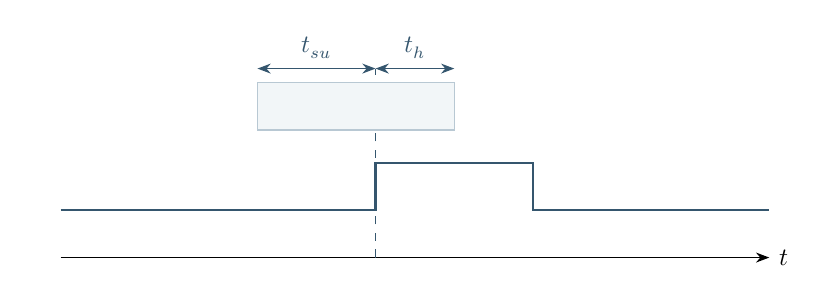
\begin{tikzpicture}[x=10mm,y=6mm]
\draw[->] (0,0)--(9,0) node[right] {$t$};
\draw[ThemeMain,thick] (0,1)--(4,1)--(4,2)--(6,2)--(6,1)--(9,1);
\node[left] at (0,1.4){时钟};
\draw[dashed,ThemeMain] (4,0)--(4,4);
\fill[ThemeBack] (2.5,2.7) rectangle (5,3.7);
\draw[ThemeBorder] (2.5,2.7) rectangle (5,3.7);
\node at (3.75,3.2){输入保持稳定};
\draw[<->,ThemeMain] (2.5,4)--(4,4) node[midway,above] {$t_{su}$};
\draw[<->,ThemeMain] (4,4)--(5,4) node[midway,above] {$t_h$};
\end{tikzpicture}
\end{center}
异步复位的释放也有恢复、移除等时序要求。常用“异步断言、同步释放”：两级触发器的异步端同时接受外部复位，释放后第一级装入 $1$、第二级再采样第一级，使本地复位按时钟释放。
\begin{lstlisting}
reg [1:0] reset_pipe;
always @(posedge clk or negedge rst_async_n) begin
  if (!rst_async_n) reset_pipe <= 2'b00;
  else reset_pipe <= {reset_pipe[0], 1'b1};
end
wire rst_sync_n = reset_pipe[1];
\end{lstlisting}
两级结构降低亚稳态传播概率，不能宣称绝对消除。不同独立时钟域需要相应的释放同步。波形分析也须考虑真实传播延迟；课堂理想状态表只表示稳定状态。

\subsection{按有效边沿分析波形}
确定复位及初态，标出有效时钟边沿；按沿前输入与现态逐沿计算次态，再画出边沿之间的保持段。
\begin{infobox}{例题：JK波形的逐沿计算}
下降沿触发JK初态 $Q=0$，连续五个下降沿处的 $JK$ 依次为 $01,01,11,00,00$。
\end{infobox}
\sol 逐沿所得 $Q$ 为 $0,0,1,1,1$，其中仅第三沿翻转。共用时钟时，各触发器同时按沿前现态计算次态。

\subsection{从触发器接线逐沿画波形}
\begin{infobox}{例题：四种反馈接法与两种有效边沿}
2024秋期末回忆版，简答题8。四个触发器的接线重绘如下。为明确波形起点，规定第一个待分析上升沿前 $Q_1=Q_2=Q_3=Q_4=0$，忽略传播延迟，画出四个完整时钟周期内的输出。
\end{infobox}
\begin{center}
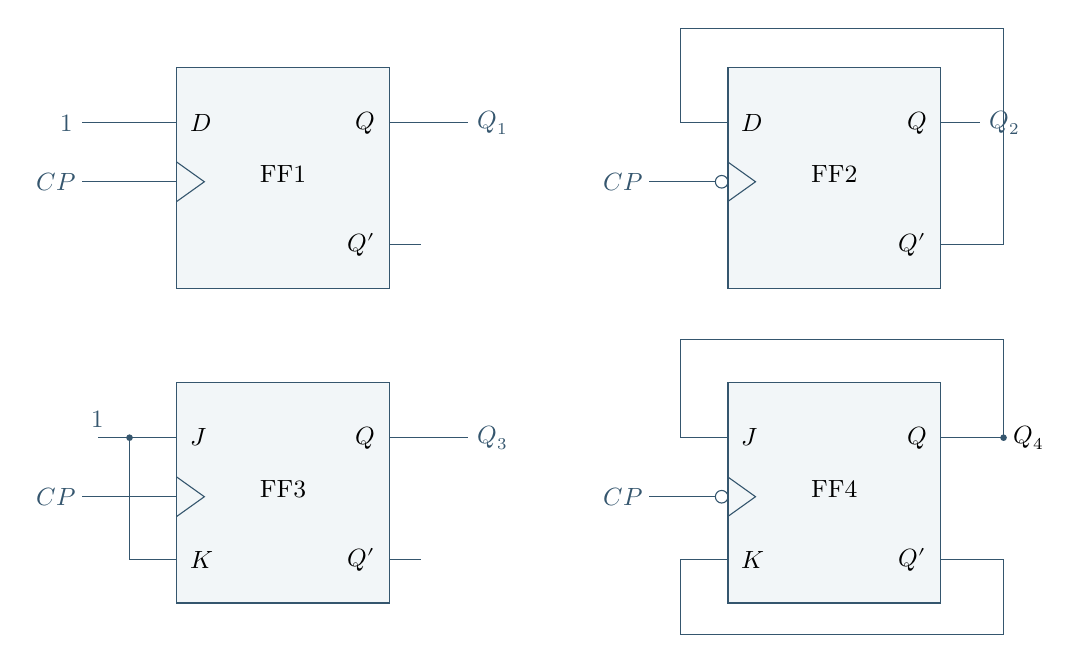
\begin{tikzpicture}[x=10mm,y=10mm,every node/.style={font=\small}]
% Four independent storage elements; triangles are clock inputs.
\foreach \x/\y/\id in {0/4/1,7/4/2,0/0/3,7/0/4}{
 \draw[ThemeMain,fill=ThemeBack] (\x,\y) rectangle ++(2.7,2.8);
 \node at (\x+1.35,\y+1.45){FF\id};
 \node[left] at (\x+2.65,\y+2.1){$Q$};
 \node[left] at (\x+2.65,\y+.55){$Q'$};
 \draw[ThemeMain] (\x,\y+1.1)--++(.35,.25)--++(-.35,.25);
}
\node[right] at (.05,6.1){$D$};
\draw[ThemeMain] (-1.2,6.1) node[left]{$1$}--(0,6.1);
\draw[ThemeMain] (-1.2,5.35) node[left]{$CP$}--(0,5.35);
\draw[ThemeMain] (2.7,6.1)--(3.7,6.1) node[right]{$Q_1$};
\draw[ThemeMain] (2.7,4.55)--(3.1,4.55);
\node[right] at (7.05,6.1){$D$};
\draw[ThemeMain] (9.7,4.55)--(10.5,4.55)--(10.5,7.3)--(6.4,7.3)--(6.4,6.1)--(7,6.1);
\draw[ThemeMain] (9.7,6.1)--(10.2,6.1) node[right]{$Q_2$};
\draw[ThemeMain] (6,5.35) node[left]{$CP$}--(6.84,5.35);
\draw[ThemeMain] (6.92,5.35) circle (.08);
\node[right] at (.05,2.1){$J$};\node[right] at (.05,.55){$K$};
\draw[ThemeMain] (-1,2.1) node[above]{$1$}--(0,2.1);
\draw[ThemeMain] (-.6,2.1)--(-.6,.55)--(0,.55);
\fill[ThemeMain] (-.6,2.1) circle (1.2pt);
\draw[ThemeMain] (-1.2,1.35) node[left]{$CP$}--(0,1.35);
\draw[ThemeMain] (2.7,2.1)--(3.7,2.1) node[right]{$Q_3$};
\draw[ThemeMain] (2.7,.55)--(3.1,.55);
\node[right] at (7.05,2.1){$J$};\node[right] at (7.05,.55){$K$};
\draw[ThemeMain] (9.7,2.1)--(10.5,2.1) coordinate (q4)--(10.5,3.35)--(6.4,3.35)--(6.4,2.1)--(7,2.1);
\node[right] at (10.5,2.1){$Q_4$};
\draw[ThemeMain] (9.7,.55)--(10.5,.55)--(10.5,-.4)--(6.4,-.4)--(6.4,.55)--(7,.55);
\draw[ThemeMain] (6,1.35) node[left]{$CP$}--(6.84,1.35);
\draw[ThemeMain] (6.92,1.35) circle (.08);
\fill[ThemeMain] (q4) circle (1.2pt);
\end{tikzpicture}
\end{center}
\sol 先读时钟三角前是否有反相圈：FF1、FF3为上升沿触发，FF2、FF4为下降沿触发。$Q'$ 表示本触发器的反相输出；反馈并未把 $Q'$ 变成时钟。
\begin{center}
\begin{tabularx}{\linewidth}{c l Y}
\toprule 输出 & 接线与次态 & 有效边沿上的行为\\\midrule
$Q_1$ & $D=1,\ Q_1^+=1$ & 第一个上升沿置一，后续保持一\\
$Q_2$ & $D=Q_2',\ Q_2^+=Q_2'$ & 每个下降沿翻转\\
$Q_3$ & $J=K=1,\ Q_3^+=Q_3'$ & 每个上升沿翻转\\
$Q_4$ & $J=Q_4,K=Q_4'$ & 每个下降沿仍保持现态\\\bottomrule
\end{tabularx}
\end{center}
最后一项必须代入JK特征方程，而非凭“存在反馈”就判为翻转：
\[
Q_4^+=JQ_4'+K'Q_4=Q_4Q_4'+Q_4Q_4=Q_4.
\]
若 $Q_4=0$，边沿前 $JK=01$，清零后仍为零；若原为 $1$，则 $JK=10$，置位后仍为一。因此本题 $Q_4$ 始终为零。

按上升沿与下降沿交替列表；非本触发器的有效边沿处须保持，不更新其状态：
\begin{center}
\begin{tabular}{c cccc}
\toprule 边沿之后 & $Q_1$&$Q_2$&$Q_3$&$Q_4$\\\midrule
初态&0&0&0&0\\
第1上升沿&1&0&1&0\\第1下降沿&1&1&1&0\\
第2上升沿&1&1&0&0\\第2下降沿&1&0&0&0\\
第3上升沿&1&0&1&0\\第3下降沿&1&1&1&0\\
第4上升沿&1&1&0&0\\第4下降沿&1&0&0&0\\\bottomrule
\end{tabular}
\end{center}
\begin{center}
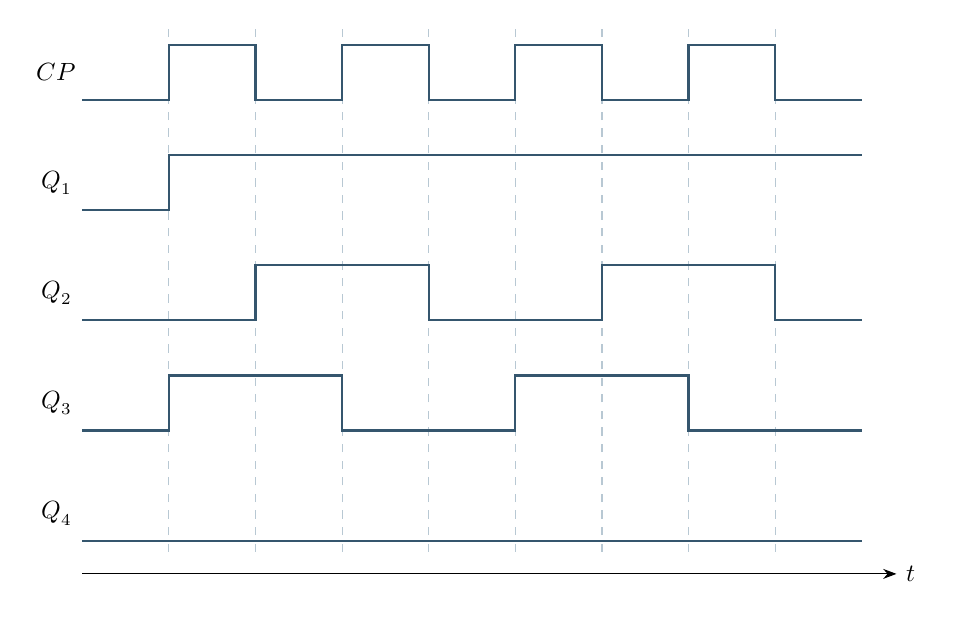
\begin{tikzpicture}[x=11mm,y=7mm,every node/.style={font=\small}]
\foreach \x in {1,...,8}\draw[ThemeBorder,dashed] (\x,-.2)--(\x,9.3);
\foreach \y/\lab in {8/CP,6/Q_1,4/Q_2,2/Q_3,0/Q_4}
 {\node[left] at (0,\y+.5){$\lab$};}
\draw[ThemeMain,thick] (0,8)--(1,8)--(1,9)--(2,9)--(2,8)--(3,8)--(3,9)--(4,9)--(4,8)--(5,8)--(5,9)--(6,9)--(6,8)--(7,8)--(7,9)--(8,9)--(8,8)--(9,8);
\draw[ThemeMain,thick] (0,6)--(1,6)--(1,7)--(9,7);
\draw[ThemeMain,thick] (0,4)--(2,4)--(2,5)--(4,5)--(4,4)--(6,4)--(6,5)--(8,5)--(8,4)--(9,4);
\draw[ThemeMain,thick] (0,2)--(1,2)--(1,3)--(3,3)--(3,2)--(5,2)--(5,3)--(7,3)--(7,2)--(9,2);
\draw[ThemeMain,thick] (0,0)--(9,0);
\draw[->] (0,-.6)--(9.4,-.6) node[right]{$t$};
\end{tikzpicture}
\end{center}
波形由表中状态连成，输出仅在自身有效边沿跳变。理想图中省略 $t_{CQ}$，实际输出应在边沿之后经过传播延迟才改变。回忆版图中的短起始线不能替代明确初态；若分析起点移到已有若干脉冲之后，须先确定该点状态，再重复同样方法。


\chapterpage{寄存器、计数器与节拍发生器}
\subsection{基本寄存器与数据传送}
\term{寄存器}用一组触发器存储有限位代码，$n$ 位寄存器通常用 $n$ 个一位触发器。写入、保持、复位改变或控制内部状态；读出把已存状态送到外部，通常不改变内部状态。

设并行输入 $\symbf D$、装载使能 $LD$，在有效时钟沿
\[
\symbf Q^+=LD\cdot\symbf D+LD'\symbf Q,
\]
乘法和加法逐位按逻辑运算解释。输出使能控制三态读出时，禁用的是对总线的驱动，而非寄存器内容。输出与门控制的禁用值为零，则与三态读出的高阻不同。

寄存器间经公共总线传送数据时，源寄存器输出使能决定总线来源，目的寄存器装载使能决定本沿是否接收数据。源使能和目的装载应保持到所需的建立、保持时间之后；读出使能不能代替写入时钟。

\subsection{累加器与并行接口}
\term{累加器}将寄存器内容 $X$ 与输入 $Y$ 相加，并把结果重新存入 $X$。若先清零，每次累加使能 $AD=1$ 时 $X^+=X+Y$（此处为算术加法）；$AD=0$ 时保持。

另一方案允许直接装载第一操作数，优先级为装载、累加、保持：
\[
X^+=\begin{cases}Y,&LD=1,\\X+Y,&LD=0,AD=1,\\X,&LD=AD=0.\end{cases}
\]
该方案用选择器决定寄存器输入，无须以清零作为每次运算的第一步。固定宽度累加须另行处理进位或溢出。并行输入输出接口用寄存器保存数据，使总线上短暂出现的数据在外部设备读出期间保持稳定。

\subsection{移位寄存器及串并转换}
\term{移位寄存器}在每个有效边沿把各位数据向规定方向移动一位。按 $Q_{n-1}\cdots Q_0$ 从左到右书写，右移为
\[
\symbf Q^+=\{R_{\mathrm{in}},Q_{n-1},\ldots,Q_1\},
\]
左移为
\[
\symbf Q^+=\{Q_{n-2},\ldots,Q_0,L_{\mathrm{in}}\}.
\]
串行输入端分别补入右移时最高位、左移时最低位。右移通过串行输入装入完整数码时，应按最低位到最高位送入；左移则按最高位到最低位送入。

\term{串入串出}（SISO）可作延迟链，串入并出（SIPO）进行串到并转换，并入串出（PISO）进行并到串转换，并入并出（PIPO）进行整字传送。若在第一个沿装入第一级，$n$ 位链的末级在第 $n$ 个沿出现该位；相对第一级的输出时刻相差 $n-1$ 个周期。讨论“延迟 $n$ 周期”时须明确以输入准备时刻还是首次采样时刻为起点。

\begin{lstlisting}
module shift4(
  input wire clk, clr,
  input wire [1:0] mode,
  input wire [3:0] d,
  input wire rin, lin,
  output reg [3:0] q
);
  always @(posedge clk) begin
    if (clr) q <= 4'b0000;
    else case (mode)
      2'b00: q <= q;
      2'b01: q <= {rin, q[3:1]};
      2'b10: q <= {q[2:0], lin};
      2'b11: q <= d;
      default: q <= q;
    endcase
  end
endmodule
\end{lstlisting}
上述模型为高有效同步清零，不能直接当作低有效异步清零的74LS194。双向移位寄存器的并行装载、左移、右移需互斥，或由模式代码给出明确优先级。若写成独立使能的加权或形式，还须补上全禁用时的保持项。

\subsection{环形与扭环形计数器}
右移寄存器把最低位反馈到串行输入，可组成\term{环形计数器}。四位单一有效位循环为
\[
1000\to0100\to0010\to0001\to1000.
\]
在该循环中，$n$ 位寄存器得到 $n$ 个状态，各位直接给出依次有效的节拍。普通结构不能保证从任意状态进入单一有效位循环：$0000$、$1111$ 为固定点，另有多有效位循环，故须预置或增加恢复逻辑。

把最低位的反反馈到右移串行输入构成\term{扭环形计数器}（Johnson counter）。四位有效循环为
\[
0000\to1000\to1100\to1110\to1111\to0111\to0011\to0001\to0000.
\]
它用 $n$ 位形成 $2n$ 个有效状态，相邻有效状态仅改变一位。四位时八个节拍输出可取
\begin{align*}
Y_0&=Q_3'Q_0',&Y_1&=Q_3Q_2',&Y_2&=Q_2Q_1',&Y_3&=Q_1Q_0',\\
Y_4&=Q_3Q_0,&Y_5&=Q_3'Q_2,&Y_6&=Q_2'Q_1,&Y_7&=Q_1'Q_0.
\end{align*}
两输入译码即可区分有效状态。但存在其他循环，通常也需要初始清零或自恢复。单比特状态变化减少译码过渡问题，不意味着任意连接、任意输入条件和复位瞬态都无冒险。

\subsection{同步二进制计数器}
\term{计数器}按输入脉冲循环经过预定状态，稳定循环的状态数称为\term{模}，记为 $N$。用 $n$ 个触发器最多有 $2^n$ 个状态，但不代表每种计数器都使用全部状态。

\term{同步计数器}的全部触发器共用外部时钟。二进制递增加法计数中，最低位每次翻转；第 $i$ 位只有当全部低位为 $1$ 时翻转。以 $Q_0$ 为最低位、$EN$ 为计数使能，可取
\[
T_0=EN,\qquad T_i=EN\prod_{j=0}^{i-1}Q_j\quad(i\ge1),\qquad Q_i^+=Q_i\oplus T_i.
\]
用D实现时令 $D_i=Q_i^+$，用JK实现时令 $J_i=K_i=T_i$。

同步计数器不产生逐级时钟延迟的累积，但仍有时钟到输出延迟、组合逻辑延迟及建立时间。简化时钟周期条件为
\[
T_{\mathrm{clk}}\ge t_{CQ,\max}+t_{\mathrm{logic},\max}+t_{su}
\]
并应另计时钟偏斜与裕量。最小路径也须满足保持约束。多位输出的传播时间不完全一致，其组合译码仍可能出现毛刺。

\begin{lstlisting}
module counter4(
  input wire clk, clr, load, enp, ent, up,
  input wire [3:0] d,
  output reg [3:0] q,
  output wire rco
);
  always @(posedge clk) begin
    if (clr) q <= 4'd0;
    else if (load) q <= d;
    else if (enp && ent) begin
      if (up) q <= q + 4'd1;
      else q <= q - 4'd1;
    end
  end
  assign rco = ent && (up ? (q == 4'd15) : (q == 4'd0));
endmodule
\end{lstlisting}
该模型的控制优先级是同步清零、同步装载、计数、保持。递增终值为 $15$，递减终值为 $0$；\code{rco} 是当前终值指示，不是一个自动保持一个周期的寄存输出。

十进制递增计数使 $0,1,\ldots,9$ 循环，计到 $9$ 后下一沿回零，终值判断也改为 $9$。余3十进制计数使代码 $3,4,\ldots,12$ 循环，复位装入 $3$，$12$ 后回到 $3$，终值判断为 $12$。若允许装载非法代码，须说明是限制输入，还是规定非法状态恢复。

\subsection{异步行波计数器与状态分析}
\term{异步计数器}的外部时钟常只接最低位触发器，后续时钟由前一级输出提供，因此状态沿逐级传播。下降沿T$'$触发器级联、后一时钟接前一级 $Q$，得到二进制递增计数；改变边沿或连接 $Q'$ 会改变计数方向，不能只凭“T触发器级联”判定方向。

三位递增行波从 $011$ 到 $100$ 时，真实过渡可能为
\[
011\to010\to000\to100.
\]
中间组合不是稳定计数状态，却可使外部译码产生错误短脉冲。累积传播延迟约随级数增加，各位稳定分频频率依次为 $f_{\mathrm{clk}}/2,f_{\mathrm{clk}}/4,\ldots$。

分析异步电路时，应逐级判断\textbf{是否收到有效边沿}；仅满足 $J=K=1$ 不代表本次外部时钟会让所有级翻转。表中次态要给出一次外部脉冲传播完成后的稳定结果，波形还须标出级间先后。

\subsection{模6计数器的完整分析}
\begin{infobox}{例题：由D驱动方程判断功能及自启动}
三位状态为 $Q_2Q_1Q_0$，共用上升沿时钟，驱动方程为
\[
D_0=Q_0',\quad D_1=Q_1Q_0'+Q_2'Q_1'Q_0,\quad
D_2=Q_2Q_0'+Q_1Q_0.
\]
\end{infobox}
\sol 对每个现态代入，得到
\begin{center}
\begin{tabular}{cc cc}
\toprule 现态&次态&现态&次态\\\midrule
000&001&100&101\\001&010&101&000\\010&011&110&111\\011&100&111&100\\\bottomrule
\end{tabular}
\end{center}
有效循环为 $000\to001\to010\to011\to100\to101\to000$，故是模6加法计数器。未用状态 $110\to111\to100$，$111\to100$，能在有限脉冲后进入有效循环，因而在状态转移意义下可自启动。自启动不等于有确定上电初相位，确定相位仍须复位。

\subsection{节拍电位与节拍脉冲}
\term{节拍发生器}在每个周期内产生按次序有效的一组控制信号，可由模计数器加译码器、环形计数器或扭环形计数器构成。$N$ 个等长状态各占一个时钟周期时，每条单状态译码线的重复周期为 $NT_{\mathrm{clk}}$。

\term{节拍电位}持续一段控制窗口，例如指定源数据或操作方式；\term{节拍脉冲}提供具体执行边沿，例如装载寄存器。节拍电位应覆盖执行边沿及所需建立、保持时间。译码生成的脉冲含有传播延迟，不能按理想状态图直接当作可靠时钟。

课件自恢复环形节拍核心可写成
\[
Q_0^+=Q_1,\quad Q_1^+=Q_2,\quad Q_2^+=Q_3,\quad
Q_3^+=(Q_3+Q_2+Q_1)'.
\]
$0000$ 下一沿进入 $1000$，之后形成四个单一有效位的循环。对任意初态还应逐项检查；$Q_3$ 的反馈不是普通环形的 $Q_0$。用SR锁存器把某两个节拍的置位、复位事件转成较长的控制电位时，须保证两个控制输入不会同时有效，并按器件实际极性连接。

\subsection{由JK接线识别同步移位寄存器}
\begin{infobox}{例题：三触发器串联电路的六拍状态}
2024秋期末回忆版，分析题2。电路初态 $Q_0=Q_1=Q_2=0$，共用上升沿时钟。六个采样沿的输入 $X$ 依次为 $1,0,1,0,0,1$。求逐拍输出并判断功能。
\end{infobox}
\begin{center}
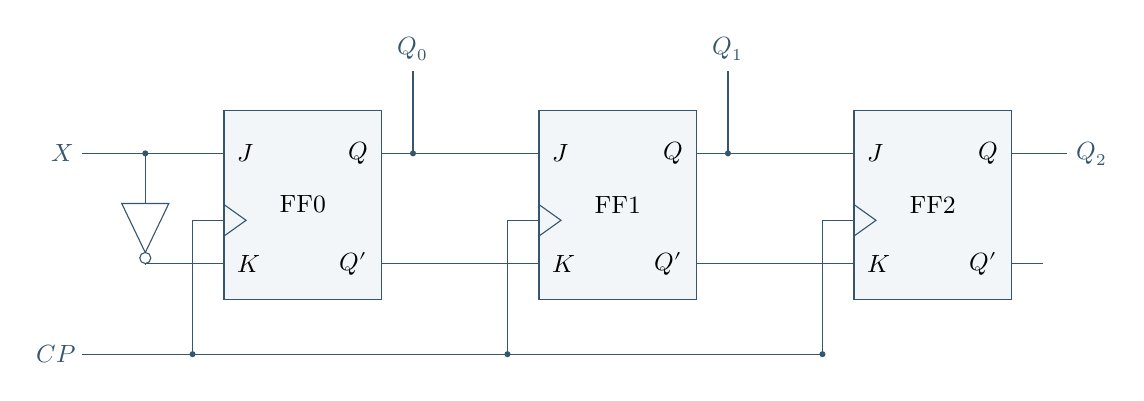
\begin{tikzpicture}[x=10mm,y=10mm,every node/.style={font=\small}]
\foreach \x/\k in {1/0,5/1,9/2}{
 \draw[ThemeMain,fill=ThemeBack] (\x,0) rectangle ++(2,2.4);
 \node at (\x+1,1.2){FF\k};
 \node[right] at (\x+.05,1.85){$J$};\node[right] at (\x+.05,.45){$K$};
 \node[left] at (\x+1.95,1.85){$Q$};\node[left] at (\x+1.95,.45){$Q'$};
 \draw[ThemeMain] (\x,.8)--++(.28,.2)--++(-.28,.2);
 \draw[ThemeMain] (\x-.4,-.7)--(\x-.4,1)--(\x,1);
 \fill[ThemeMain] (\x-.4,-.7) circle (1.1pt);
}
\draw[ThemeMain] (-.8,1.85) node[left]{$X$}--(1,1.85);
\node[not gate US,draw=ThemeMain,minimum width=7mm,rotate=-90] (inv) at (0,1) {};
\draw[ThemeMain] (0,1.85)--(inv.input);
\draw[ThemeMain] (inv.output)|-(1,.45);
\fill[ThemeMain] (0,1.85) circle (1.1pt);
\foreach \a/\b/\k in {3/5/0,7/9/1}{
 \draw[ThemeMain] (\a,1.85)--(\b,1.85);
 \draw[ThemeMain] (\a,.45)--(\b,.45);
 \draw[ThemeMain] (\a+.4,1.85)--(\a+.4,2.9) node[above]{$Q_{\k}$};
 \fill[ThemeMain] (\a+.4,1.85) circle (1.1pt);
}
\draw[ThemeMain] (11,1.85)--(11.7,1.85) node[right]{$Q_2$};
\draw[ThemeMain] (11,.45)--(11.4,.45);
\draw[ThemeMain] (-.8,-.7) node[left]{$CP$}--(8.6,-.7);
\end{tikzpicture}
\end{center}
\sol 先读取接线，而非直接把三个触发器认作计数器：
\[
J_0=X,\ K_0=X';\qquad
J_1=Q_0,\ K_1=Q_0';\qquad
J_2=Q_1,\ K_2=Q_1'.
\]
对一般接法 $J=U,K=U'$，代入特征方程得到 $Q^+=UQ'+UQ=U$。所以三组JK在这里都实现D功能：
\[
Q_0^+=X,\qquad Q_1^+=Q_0,\qquad Q_2^+=Q_1.
\]
右端全部取同一沿前的旧状态，不能让第二级读到本沿刚更新的 $Q_0$。
\begin{center}
\begin{tabular}{c c c c}
\toprule 脉冲 & 输入 $X$ & 沿前 $Q_2Q_1Q_0$ & 沿后 $Q_2Q_1Q_0$\\\midrule
1&1&000&001\\2&0&001&010\\3&1&010&101\\
4&0&101&010\\5&0&010&100\\6&1&100&001\\\bottomrule
\end{tabular}
\end{center}
输出波形如下，输入在采样沿之间改变，以避开建立、保持窗口：
\begin{center}
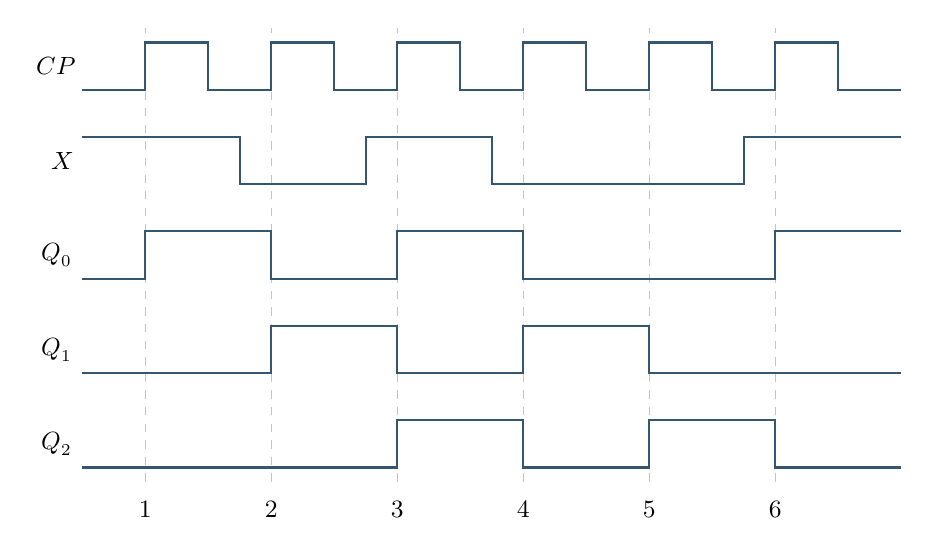
\begin{tikzpicture}[x=8mm,y=6mm,every node/.style={font=\small}]
\foreach \x in {1,3,5,7,9,11}\draw[ThemeBorder,dashed] (\x,1.7)--(\x,11.3);
\foreach \y/\lab in {10/CP,8/X,6/Q_0,4/Q_1,2/Q_2}
 {\node[left] at (0,\y+.5){$\lab$};}
\draw[ThemeMain,thick] (0,10)--(1,10)--(1,11)--(2,11)--(2,10)--(3,10)--(3,11)--(4,11)--(4,10)--(5,10)--(5,11)--(6,11)--(6,10)--(7,10)--(7,11)--(8,11)--(8,10)--(9,10)--(9,11)--(10,11)--(10,10)--(11,10)--(11,11)--(12,11)--(12,10)--(13,10);
\draw[ThemeMain,thick] (0,9)--(2.5,9)--(2.5,8)--(4.5,8)--(4.5,9)--(6.5,9)--(6.5,8)--(10.5,8)--(10.5,9)--(13,9);
\draw[ThemeMain,thick] (0,6)--(1,6)--(1,7)--(3,7)--(3,6)--(5,6)--(5,7)--(7,7)--(7,6)--(11,6)--(11,7)--(13,7);
\draw[ThemeMain,thick] (0,4)--(3,4)--(3,5)--(5,5)--(5,4)--(7,4)--(7,5)--(9,5)--(9,4)--(13,4);
\draw[ThemeMain,thick] (0,2)--(5,2)--(5,3)--(7,3)--(7,2)--(9,2)--(9,3)--(11,3)--(11,2)--(13,2);
\foreach \x/\k in {1/1,3/2,5/3,7/4,9/5,11/6}
 {\node[below] at (\x,1.5){第\k 沿};}
\end{tikzpicture}
\end{center}
该电路是三位同步串入并出移位寄存器，也可从 $Q_2$ 串行读出。若 $X[k]$ 表示第 $k$ 沿采样的输入，则 $Q_2[k]=X[k-2]$（$k\ge3$）。首个输入在第1沿进入第一级，在第3沿到达第三级；从首沿到末沿相隔两个周期，不能与“经过三级存储”混为三周期。


\chapterpage{同步状态机的分析与设计}
\subsection{有限状态机、Mealy与Moore模型}
\term{有限状态机}（FSM）由有限状态集合、输入集合、次态函数、输出函数及指定初态构成。电路状态总结了决定未来行为所需的历史信息。数字控制电路通常持续运行，不要求具有终态或到终态停止。

\term{Mealy型}为 $\symbf Q^+=F(\symbf Q,\symbf X)$、$\symbf Z=G(\symbf Q,\symbf X)$；\term{Moore型}的次态仍可依赖输入，输出为 $\symbf Z=G(\symbf Q)$。Mealy输出标在边的“输入/输出”上，Moore输出标在状态内。Mealy输入变化可在同一周期改变输出；Moore组合译码也可能在状态位交接时有毛刺，需要寄存输出时应明确另加寄存器。

\begin{infobox}{例题：带使能的两位计数状态机}
次态为 $Q_0^+=Q_0\oplus EN$、$Q_1^+=Q_1\oplus(Q_0EN)$。当 $EN=0$ 时保持，当 $EN=1$ 时 $00\to01\to10\to11\to00$。
\end{infobox}
若 $MAX=Q_1Q_0EN$，输出与现态和输入有关，为Mealy型；若 $MAX_S=Q_1Q_0$，输出只由现态决定，为Moore型。前者表示当前允许进位的终值条件，后者表示已处于最大状态。

\subsection{从需求建立原始状态表}
\begin{infobox}{方法：同步时序电路设计流程}
\begin{enumerate}
\item 规定输入、输出、采样边沿、初态及输出的时间含义。
\item 根据必须记忆的历史建立原始状态图和状态表，覆盖每个状态的全部输入。
\item 删除确定不可达状态，合并等价状态，保留功能及初态意义。
\item 分配状态编码，选择触发器，建立编码后的次态与输出表。
\item 由激励表求驱动函数，化简并实现；核对非法状态的恢复及输出。
\item 通过状态表、输入序列和边界条件验证，再检查物理时序。
\end{enumerate}
\end{infobox}
状态划分应仅保留需要的历史。例如串行二进制加法器每次输入 $X_1,X_2$，只需记住前一位的进位 $c$。两个状态分别代表无进位、有进位，输出和次态为
\[
Z=X_1\oplus X_2\oplus c,\qquad c^+=X_1X_2+(X_1\oplus X_2)c.
\]
位流须从最低位开始，初态 $c=0$。同步模5可逆计数器则需五个计数状态；输入 $X=0$ 时递增、$X=1$ 时递减，输出可定义为“状态4且递增，或状态0且递减”的进借位条件。输出的含义与状态转移时刻必须一并说明。

\subsection{101序列检测与重叠}
序列检测每个有效时钟沿接收一个输入 $X$，识别最近输入是否形成目标串。状态表示“已接收串的后缀中，与目标前缀匹配的最长部分”。设三状态 $S_0$（无非空匹配）、$S_1$（匹配1）、$S_2$（匹配10）。
\begin{center}
\begin{tabular}{c cc}
\toprule 现态 & $X=0$时次态/输出 & $X=1$时次态/输出\\\midrule
$S_0$&$S_0/0$&$S_1/0$\\
$S_1$&$S_2/0$&$S_1/0$\\
$S_2$&$S_0/0$&$S_1/1$\\\bottomrule
\end{tabular}
\end{center}
上表是\term{可重叠}Mealy检测器。完成 $101$ 后，末尾的 $1$ 可作为下一次匹配的起点，因此回到 $S_1$。输入 $10101$ 在第3、第5位各输出一次。
\begin{center}
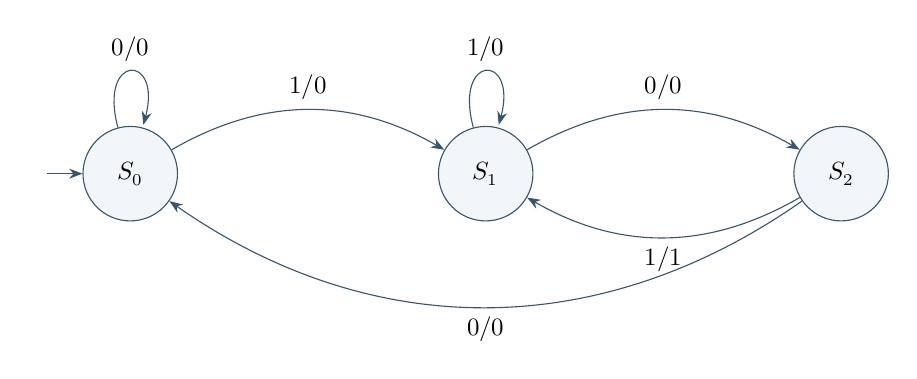
\begin{tikzpicture}[node distance=33mm]
\node[state,initial,initial text={}] (s0) {$S_0$};
\node[state,right=of s0] (s1) {$S_1$};
\node[state,right=of s1] (s2) {$S_2$};
\path (s0) edge[loop above] node {$0/0$} (s0)
 edge[bend left] node[above] {$1/0$} (s1)
 (s1) edge[loop above] node {$1/0$} (s1)
 edge[bend left] node[above] {$0/0$} (s2)
 (s2) edge[bend left] node[below] {$1/1$} (s1)
 edge[bend left=35] node[below] {$0/0$} (s0);
\end{tikzpicture}
\end{center}
\term{不可重叠}检测器在完成后丢弃本次已使用的三位，将 $S_2$ 在 $X=1$ 时的次态改为 $S_0$，仍输出 $1$。此时 $10101$ 只在第3位报告，不能在第5位复用上一匹配的末位。

若采用Moore型，另设 $S_3$ 表示已检测到 $101$，$S_3$ 的输出为 $1$，其他状态为 $0$。可重叠时 $S_3$ 收到 $0$ 转到 $S_2$，收到 $1$ 转到 $S_1$；不可重叠时，收到 $0$ 转到 $S_0$、收到 $1$ 转到 $S_1$。两种模型的输出时间须在波形中标明，不能把“进入检测状态”与“由当前边产生检测输出”混写。

\subsection{等价状态与隐含表法}
对于完全给定的确定状态机，两个状态\term{等价}，是指从它们出发，对任意后续输入序列产生相同输出序列。判别需同时满足：每个输入下当前输出相同；相应次态也等价。当前输出相同仅是必要条件。

\term{隐含表法}对全部不同状态对建立三角表：先把存在输出差异的状态对标为不等价；对其他状态对记录其各输入下的次态对。若记录中任何次态对已不等价，当前对也不等价。反复传播到不再变化，未被排除的状态对等价。只互相依赖且没有矛盾输出的封闭链可以保留。等价关系具有传递性，最后按最大等价类合并。
\begin{infobox}{例题：课件七状态表的化简}
表中的每项为“次态/输出”。
\begin{center}
\begin{tabular}{c cc}
\toprule 现态&$X=0$&$X=1$\\\midrule
a&c/0&b/1\\b&f/0&a/1\\c&d/0&g/0\\d&d/1&e/0\\
e&c/0&e/1\\f&d/0&g/0\\g&c/1&d/0\\\bottomrule
\end{tabular}
\end{center}
\end{infobox}
\sol 输出向量先分为 $\{a,b,e\}$（$0,1$）、$\{c,f\}$（$0,0$）、$\{d,g\}$（$1,0$）。$c,f$ 的各次态完全相同，故等价。$(a,b)$ 依赖 $(c,f)$ 和自身，$(a,e)$、$(b,e)$ 依赖同组内状态对，因此三者等价。

$d,g$ 虽输出相同，但在 $X=0$ 时分别转到 $d,c$，两者输出向量不同，故 $d,g$ 不等价。令 $q_1=\{a,b,e\},q_2=\{c,f\},q_3=\{d\},q_4=\{g\}$，得
\begin{center}
\begin{tabular}{c cc}
\toprule 现态&$X=0$&$X=1$\\\midrule
$q_1$&$q_2/0$&$q_1/1$\\$q_2$&$q_3/0$&$q_4/0$\\
$q_3$&$q_3/1$&$q_1/0$\\$q_4$&$q_2/1$&$q_3/0$\\\bottomrule
\end{tabular}
\end{center}
完全给定机的等价类互不重叠；不完全定义状态机的兼容关系需要其他处理，本讲义按课件主要范围讨论完全给定状态表。

\subsection{余3码串行误码检测}
\begin{infobox}{例题：每四位判断一次的码制检测器}
余3码最高位先输入，每接收第4位时判定该组是否有效。有效码为 $0011$ 至 $1100$；非法码输出 $Z=1$，有效码输出 $Z=0$，随后重新接收下一组。
\end{infobox}
\sol 建立前缀树：初态 $\varepsilon$ 代表已接收零位；每个输入形成下一层前缀。收到前三位时各有 $2,4,8$ 个可能前缀，第四位只输出判断并返回初态，原始状态总数为 $1+2+4+8=15$。

最底层三个比特的前缀，其第四位输出为：$000$ 和 $111$ 对 $0,1$ 均输出 $1$；$001$ 输出 $1,0$；$010,011,100,101$ 均输出 $0,0$；$110$ 输出 $0,1$。令它们的等价类为 $A,B,C,D$。前两位 $01,10$ 均向 $C,C$ 转移，亦可合并。保留各接收位数的阶段，得到十状态表：
\begin{center}
\begin{tabular}{l cc}
\toprule 状态意义&$X=0$时次态/输出&$X=1$时次态/输出\\\midrule
$\varepsilon$（零位）&$P_0/0$&$P_1/0$\\
$P_0$（前缀0）&$P_{00}/0$&$P_{01,10}/0$\\
$P_1$（前缀1）&$P_{01,10}/0$&$P_{11}/0$\\
$P_{00}$&$A/0$&$B/0$\\
$P_{01,10}$&$C/0$&$C/0$\\
$P_{11}$&$D/0$&$A/0$\\
$A$（000或111）&$\varepsilon/1$&$\varepsilon/1$\\
$B$（001）&$\varepsilon/1$&$\varepsilon/0$\\
$C$（010、011、100或101）&$\varepsilon/0$&$\varepsilon/0$\\
$D$（110）&$\varepsilon/0$&$\varepsilon/1$\\\bottomrule
\end{tabular}
\end{center}
前三位收到时输出一直为零，第四位输出才有判断意义。若接口还需区分“尚未判断”与“有效码”，可添加完成标志。帧边界必须由复位、有效使能或输入协议保证；不能把任意连续四位滑动窗口与分组检测混为一谈。

\subsection{状态编码与触发器数量}
$N$ 个不同状态采用紧凑二进制编码时，最少位数为
\[
k=\lceil\log_2N\rceil,\qquad 2^{k-1}<N\le2^k\quad(N>1).
\]
$N=1$ 时可无状态存储位，也可按实现约定保留寄存位。使用更多状态位可能简化组合逻辑，如独热编码用每个状态一个位；最少触发器数量不必给出最小实现总代价。

课件的相邻编码规则是启发式方法：同一输入下次态相同的现态尽量相邻；同一现态在不同输入下的次态尽量相邻；输出相同的现态也可尽量相邻。这些目标可能冲突，通常优先考虑驱动函数化简，并让初态便于复位。编码必须互不相同，不能为满足相邻性把两个非等价状态编为同一码。

\subsection{110检测器：从状态化简到JK实现}
\begin{infobox}{例题：JK触发器实现110序列检测}
每个有效边沿接收一位 $X$。识别到连续子串 $110$ 时输出一次 $Z=1$，采用Mealy输出。
\end{infobox}
\sol 设 $S_0$ 为无匹配，$S_1$ 为末尾1，$S_2$ 为末尾11。若另设完成状态 $S_3$，它下一输入的行为与 $S_0$ 相同，可合并。最简状态表为
\begin{center}
\begin{tabular}{c cc}
\toprule 现态&$X=0$&$X=1$\\\midrule
$S_0$&$S_0/0$&$S_1/0$\\$S_1$&$S_0/0$&$S_2/0$\\$S_2$&$S_0/1$&$S_2/0$\\\bottomrule
\end{tabular}
\end{center}
分配 $S_0=00,S_1=10,S_2=11$，状态变量为 $Q_2Q_1$。逐位按JK激励表填表，未用编码 $01$ 先作化简无关状态：
\begin{center}
\begin{tabular}{c cc cc cc cc c}
\toprule $X$&$Q_2$&$Q_1$&$Q_2^+$&$Q_1^+$&$J_2$&$K_2$&$J_1$&$K_1$&$Z$\\\midrule
0&0&0&0&0&0&$\times$&0&$\times$&0\\
0&1&0&0&0&$\times$&1&0&$\times$&0\\
0&1&1&0&0&$\times$&1&$\times$&1&1\\
1&0&0&1&0&1&$\times$&0&$\times$&0\\
1&1&0&1&1&$\times$&0&1&$\times$&0\\
1&1&1&1&1&$\times$&0&$\times$&0&0\\\bottomrule
\end{tabular}
\end{center}
化简得到
\[
J_2=X,\quad K_2=X',\quad J_1=XQ_2,\quad K_1=X',\quad Z=X'Q_1.
\]
将实际驱动代回特征方程，检查所有状态：
\begin{align*}
Q_2^+&=XQ_2'+XQ_2=X,\\
Q_1^+&=XQ_2Q_1'+XQ_1=X(Q_2+Q_1).
\end{align*}
未用 $01$ 在 $X=0$ 时进入 $00$，在 $X=1$ 时进入 $11$，一步即可恢复。然而在 $01,X=0$ 时原输出 $Z=1$，恢复期间可能给出一次无效检测。若要求非法状态不报检测，可把输出改为 $Z=X'Q_2Q_1$；合法状态上功能不变。

\begin{lstlisting}
module detect110(
  input wire clk, rst_n, x,
  output wire z
);
  reg q2, q1;
  always @(posedge clk or negedge rst_n) begin
    if (!rst_n) begin q2 <= 1'b0; q1 <= 1'b0; end
    else begin
      q2 <= x;
      q1 <= x & (q2 | q1);
    end
  end
  assign z = (~x) & q2 & q1;
endmodule
\end{lstlisting}
此代码按化简次态用D触发器表达，与上述JK方案的状态行为相同。$z$ 为组合Mealy输出，在采样边沿前当 $x=0$ 且现态为 $11$ 时有效；边沿后状态回零。若需沿后保持一个完整周期的检测脉冲，应另用寄存器在该沿采样条件，并说明输出接口的时序。

\subsection{非法状态、自启动与功能验证}
\term{自启动}是电路能从未用编码在有限更新后进入有效工作集合。它不是有确定的初态，也不能保证恢复途中输出正确。设计应分别检查：所有非法编码的实际次态；是否存在非法闭环或固定点；恢复输出是否允许；恢复是否依赖特定输入。

状态机验证可将编码实现的每个合法状态、每个输入组合，与抽象状态表逐项比较，再使用有代表性的连续输入验证历史意义。例如110检测输入 $1110$ 只在最后一个 $0$ 处报告，因为最后三位是 $110$；输入 $110110$ 报告两次。非阻塞更新须用旧状态，避免在同一沿错误提前推进多个匹配阶段。

\subsection{从两级D触发器电路识别可逆计数}
\begin{infobox}{例题：含异或门与与非门的同步电路}
2024秋期末回忆版，分析题1。按下图求次态方程、输出方程、状态表及状态图。两触发器共用上升沿时钟，$Q_1Q_0$ 为从高到低的现态，$A$ 为控制输入。复位或起始状态须由外部条件确定。
\end{infobox}
\begin{center}
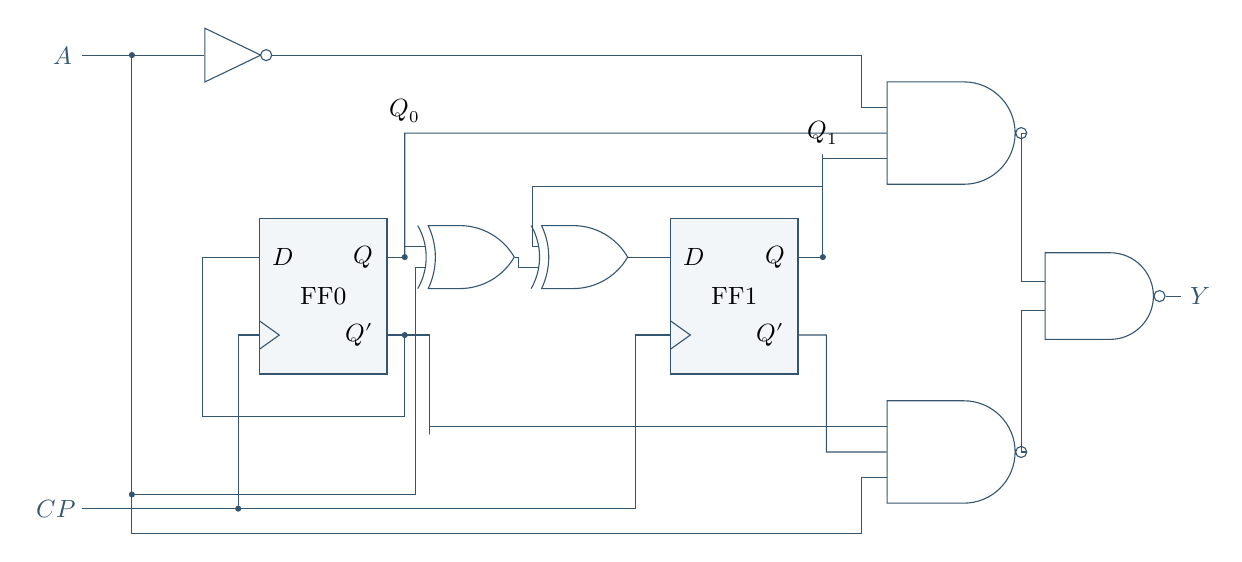
\begin{tikzpicture}[x=9mm,y=9mm,every node/.style={font=\small}]
\foreach \x/\k in {2.5/0,8.3/1}{
 \draw[ThemeMain,fill=ThemeBack] (\x,-1.1) rectangle ++(1.8,2.2);
 \node at (\x+.9,0){FF\k};
 \node[right] at (\x+.05,.55){$D$};
 \node[left] at (\x+1.75,.55){$Q$};\node[left] at (\x+1.75,-.55){$Q'$};
 \draw[ThemeMain] (\x,-.75)--++(.28,.2)--++(-.28,.2);
}
\node[xor gate US,draw=ThemeMain,logic gate inputs=nn,
 minimum width=8mm,minimum height=8mm] (x0) at (5.4,.55) {};
\node[xor gate US,draw=ThemeMain,logic gate inputs=nn,
 minimum width=8mm,minimum height=8mm] (x1) at (7.0,.55) {};
\node[not gate US,draw=ThemeMain,minimum width=8mm] (iv) at (2,3.4) {};
\node[nand gate US,draw=ThemeMain,logic gate inputs=nnn,
 minimum width=12mm,minimum height=13mm] (n0) at (12.2,2.3) {};
\node[nand gate US,draw=ThemeMain,logic gate inputs=nnn,
 minimum width=12mm,minimum height=13mm] (n1) at (12.2,-2.2) {};
\node[nand gate US,draw=ThemeMain,logic gate inputs=nn,
 minimum width=12mm,minimum height=11mm] (ny) at (14.3,0) {};
\draw[ThemeMain] (0,3.4) node[left]{$A$}--(iv.input);
\draw[ThemeMain] (iv.output)--(11.0,3.4)|-(n0.input 1);
\draw[ThemeMain] (.7,3.4)--(.7,-3.35)--(11.0,-3.35)|-(n1.input 3);
\draw[ThemeMain] (.7,-2.8)--(4.7,-2.8)|-(x0.input 2);
\fill[ThemeMain] (.7,3.4) circle (1.1pt);\fill[ThemeMain] (.7,-2.8) circle (1.1pt);
\draw[ThemeMain] (4.3,.55)--(4.55,.55) coordinate (q0)|-(x0.input 1);
\draw[ThemeMain] (q0)--(4.55,2.3)--(n0.input 2);
\node[above] at (4.55,2.3){$Q_0$};
\draw[ThemeMain] (x0.output)--(6.15,.55)|-(x1.input 2);
\draw[ThemeMain] (10.1,.55)--(10.45,.55) coordinate (q1)--(10.45,1.55)--(6.35,1.55)|-(x1.input 1);
\draw[ThemeMain] (q1)--(10.45,2.0)|-(n0.input 3);
\node[above] at (10.45,2.0){$Q_1$};
\draw[ThemeMain] (x1.output)--(8.3,.55);
\draw[ThemeMain] (4.3,-.55)--(4.55,-.55) coordinate (b0)--(4.55,-1.7)--(1.7,-1.7)--(1.7,.55)--(2.5,.55);
\draw[ThemeMain] (b0)--(4.9,-.55)--(4.9,-1.95)|-(n1.input 1);
\draw[ThemeMain] (10.1,-.55)--(10.5,-.55)--(10.5,-2.2)--(n1.input 2);
\draw[ThemeMain] (n0.output)--(13.25,2.3)|-(ny.input 1);
\draw[ThemeMain] (n1.output)--(13.25,-2.2)|-(ny.input 2);
\draw[ThemeMain] (ny.output)--(15.5,0) node[right]{$Y$};
\draw[ThemeMain] (0,-3) node[left]{$CP$}--(7.8,-3);
\draw[ThemeMain] (2.2,-3)--(2.2,-.55)--(2.5,-.55);
\draw[ThemeMain] (7.8,-3)--(7.8,-.55)--(8.3,-.55);
\foreach \p in {q0,q1,b0}\fill[ThemeMain] (\p) circle (1.1pt);
\fill[ThemeMain] (2.2,-3) circle (1.1pt);
\end{tikzpicture}
\end{center}
图中实心点表示导线相接；没有实心点的交叉线互不连接。

\sol 第一级D端接自己的反相输出，所以每沿翻转。第二级D端来自两个异或门，依次加入 $Q_0,A,Q_1$。因此
\[
Q_0^+=Q_0',\qquad Q_1^+=Q_1\oplus Q_0\oplus A.
\]
输出部分的上、下与非门分别产生 $(A'Q_0Q_1)'$ 与 $(AQ_0'Q_1')'$；再经末级与非门，由德摩根律得到
\[
Y=A'Q_0Q_1+AQ_0'Q_1'.
\]
逐项代入现态，不从输出方程推测次态：
\begin{center}
\begin{tabular}{c cc}
\toprule 现态 $Q_1Q_0$ & $A=0$：次态/$Y$ & $A=1$：次态/$Y$\\\midrule
00&01/0&11/1\\01&10/0&00/0\\
10&11/0&01/0\\11&00/1&10/0\\\bottomrule
\end{tabular}
\end{center}
\begin{center}
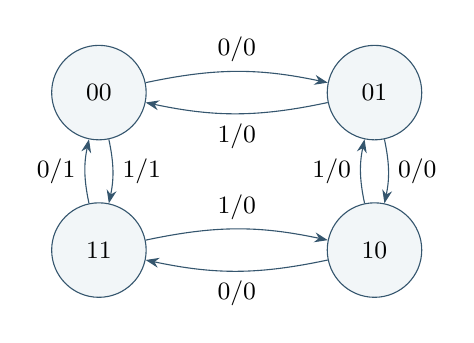
\begin{tikzpicture}[every node/.style={font=\small}]
\node[state] (s0) at (0,2){00};\node[state] (s1) at (3.5,2){01};
\node[state] (s2) at (3.5,0){10};\node[state] (s3) at (0,0){11};
\path (s0) edge[bend left=12] node[above] {0/0} (s1)
 (s1) edge[bend left=12] node[below] {1/0} (s0)
 (s1) edge[bend left=12] node[right] {0/0} (s2)
 (s2) edge[bend left=12] node[left] {1/0} (s1)
 (s2) edge[bend left=12] node[below] {0/0} (s3)
 (s3) edge[bend left=12] node[above] {1/0} (s2)
 (s3) edge[bend left=12] node[left] {0/1} (s0)
 (s0) edge[bend left=12] node[right] {1/1} (s3);
\end{tikzpicture}
\end{center}
边标记为 $A/Y$。$A=0$ 时按 $00\to01\to10\to11\to00$ 递增；$A=1$ 时反向递减。因此它是二位模4可逆计数器，$Y$ 是当前方向下的终值标志：递增时现态11有效，递减时现态00有效。由于 $Y$ 还依赖 $A$，属于Mealy输出；稳定的终值电平不等于已经存储的一周期进位脉冲。

\subsection{从多路输出波形设计JK状态机}
\begin{infobox}{例题：五拍循环的三路输出波形}
依据2024秋期末回忆版设计题2的题型改编。规定在每个上升沿后，输出 $Y_2Y_1Y_0$ 循环为
\[
000\to001\to010\to011\to101\to000\to\cdots.
\]
复位后输出000。用JK触发器实现，给出所需触发器数、状态分配、驱动方程及非法状态恢复方式。
\end{infobox}
\begin{center}
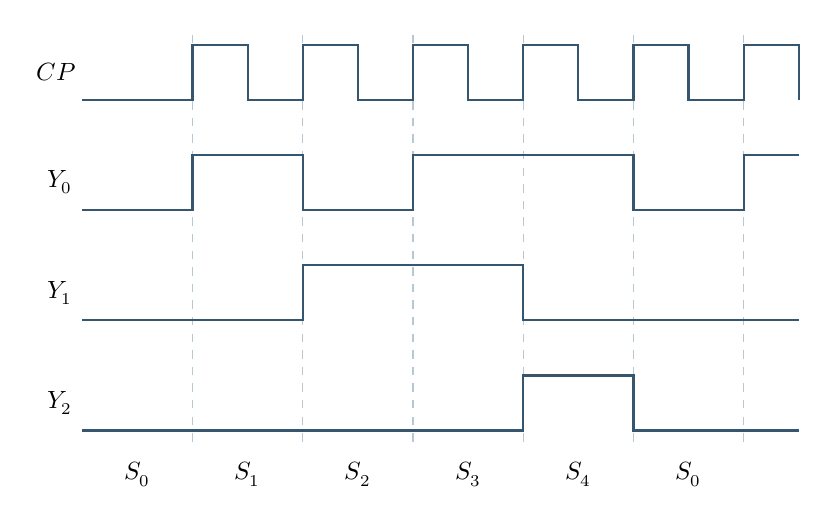
\begin{tikzpicture}[x=14mm,y=7mm,every node/.style={font=\small}]
\foreach \x in {1,...,6}\draw[ThemeBorder,dashed] (\x,-.2)--(\x,7.3);
\foreach \y/\lab in {6/CP,4/Y_0,2/Y_1,0/Y_2}
 {\node[left] at (0,\y+.5){$\lab$};}
\draw[ThemeMain,thick] (0,6)--(1,6)--(1,7)--(1.5,7)--(1.5,6)--(2,6)--(2,7)--(2.5,7)--(2.5,6)--(3,6)--(3,7)--(3.5,7)--(3.5,6)--(4,6)--(4,7)--(4.5,7)--(4.5,6)--(5,6)--(5,7)--(5.5,7)--(5.5,6)--(6,6)--(6,7)--(6.5,7)--(6.5,6);
\draw[ThemeMain,thick] (0,4)--(1,4)--(1,5)--(2,5)--(2,4)--(3,4)--(3,5)--(5,5)--(5,4)--(6,4)--(6,5)--(6.5,5);
\draw[ThemeMain,thick] (0,2)--(2,2)--(2,3)--(4,3)--(4,2)--(6.5,2);
\draw[ThemeMain,thick] (0,0)--(4,0)--(4,1)--(5,1)--(5,0)--(6.5,0);
\foreach \x/\s in {0.5/S_0,1.5/S_1,2.5/S_2,3.5/S_3,4.5/S_4,5.5/S_0}
 {\node[below] at (\x,-.4){$\s$};}
\end{tikzpicture}
\end{center}
\sol 先读有效沿之间的完整输出组合，再确定循环状态。五个输出组合各不相同，至少需要五个状态；因 $2^2<5\le2^3$，须用三个触发器。设内部状态为 $Q_2Q_1Q_0$，按自然升序分配：
\begin{center}
\begin{tabular}{c c c c}
\toprule 状态 & 内部编码 & 次态编码 & 输出 $Y_2Y_1Y_0$\\\midrule
$S_0$&000&001&000\\$S_1$&001&010&001\\
$S_2$&010&011&010\\$S_3$&011&100&011\\
$S_4$&100&000&101\\\bottomrule
\end{tabular}
\end{center}
内部编码与输出不同，尤其 $S_4$ 的编码100对应输出101，不能把输出字直接当作状态分配。规定未用编码101、110、111在下一沿回到000。根据现态与次态逐位查JK激励表：
\begin{center}
\begin{tabular}{c c cc cc cc}
\toprule 现态&次态&$J_2$&$K_2$&$J_1$&$K_1$&$J_0$&$K_0$\\\midrule
000&001&0&$\times$&0&$\times$&1&$\times$\\
001&010&0&$\times$&1&$\times$&$\times$&1\\
010&011&0&$\times$&$\times$&0&1&$\times$\\
011&100&1&$\times$&$\times$&1&$\times$&1\\
100&000&$\times$&1&0&$\times$&0&$\times$\\\bottomrule
\end{tabular}
\end{center}
再把三个非法编码的清零转移纳入驱动要求，用激励表中的无关输入化简，可得
\[
\begin{array}{lll}
J_0=Q_2',&K_0=1,\\
J_1=Q_2'Q_0,&K_1=Q_2+Q_0,\\
J_2=Q_1Q_0,&K_2=1.
\end{array}
\]
代回特征方程检查全部八个编码：
\begin{align*}
Q_0^+&=Q_2'Q_0',\\
Q_1^+&=Q_2'(Q_1'Q_0+Q_1Q_0'),\\
Q_2^+&=Q_2'Q_1Q_0.
\end{align*}
在 $Q_2=1$ 的三个非法编码中，上式全部为零，确实一步恢复000。有效状态输出可取 $Y_0=Q_0+Q_2,Y_1=Q_1,Y_2=Q_2$；若还要求恢复期间输出000，令有效编码标志 $V_s=Q_2'+Q_1'Q_0'$，再给三个输出分别与上 $V_s$。最后逐拍核对五个合法状态的输出，就得到题设波形。

回忆版原图没有标明重复周期边界，个别起始跳变也未与时钟边沿对齐。本例重新明确周期、有效边沿与初态，演示同类题的完整设计方法，不把这些补充条件当作原试题已给条件。


\chapterpage{中规模芯片与序列信号发生器}
\subsection{计数器功能表与控制优先级}
中规模芯片内部包含计数与控制逻辑，使用时以外部功能表为依据。课件常用器件如下，计数输入均须满足具体器件的有效边沿和时序要求。
\begin{center}
\begin{tabular}{l c l l}
\toprule 型号&正常计数模&装载方式&清零方式\\\midrule
74LS160&10&同步、低有效&异步、低有效\\
74LS161&16&同步、低有效&异步、低有效\\
74LS162&10&同步、低有效&同步、低有效\\
74LS163&16&同步、低有效&同步、低有效\\
74LS192&10&异步、低有效&异步、高有效\\
74LS193&16&异步、低有效&异步、高有效\\
74LS190&10&异步、低有效&无独立清零端\\
74LS191&16&异步、低有效&无独立清零端\\\bottomrule
\end{tabular}
\end{center}
74LS160--163的计数为同步上升沿，计数使能 $ENP,ENT$ 必须都为 $1$；装载不依赖两者同时启用。清零的优先级高于装载，装载高于计数，其他情况保持。同步控制需要控制电平与有效边沿共同满足；异步清零在有效电平到来后立即生效，无须等待时钟。

四位二进制型号的进位标志为 $RCO=ENT\cdot Q_DQ_CQ_BQ_A$；十进制型号在正常BCD循环中于 $9$ 给出对应终值标志。输出顺序 $Q_DQ_CQ_BQ_A$ 中 $Q_D$ 最高、$Q_A$ 最低。控制规律参考课件，并用\href{https://www.ti.com/lit/ds/symlink/sn74ls163a.pdf}{TI 74LS160A--163A资料}核验。

\subsection{反馈清零与反馈置数}
\begin{infobox}{方法：终值判断的时机}
若稳定循环要求 $0,1,\ldots,M-1$，异步清零方案通常译码 $M$，达到后立即清零；同步清零或同步装载方案须译码 $M-1$，使下一沿回零。两者稳定循环都含 $M$ 个状态，异步方案另经过极短的复位触发过渡。
\end{infobox}
以模10为例：74LS161可在出现 $1010$ 时异步清零；从初态零开始计数时，可用 $Q_DQ_B$ 的首次成立判断10，清零引脚接 $(Q_DQ_B)'$。这是在正常可达计数路径上使用部分译码；若必须从任意非法初态恢复，应检查其他状态，或使用完整 $Q_DQ_C'Q_BQ_A'$ 译码。

74LS163同步清零须在 $1001$（9）期间使清零有效，使下一沿直接回 $0000$。完整终值译码为 $Q_DQ_C'Q_B'Q_A$，同步清零引脚接其反；若在 $1010$ 才触发，下个边沿才清零，将多保留一个状态，模值成为11。

同步置数归零法令装载数据为 $0000$，$LD_n=(Q_DQ_C'Q_B'Q_A)'$，可用74LS161或163构成模10。同步装载的触发状态同样是 $9$，不能因为161具有异步清零就把它的同步装载也当作异步。

预置起点 $P$、终点 $T$ 并在 $T$ 的下一沿装回 $P$，循环状态数为 $T-P+1$。例如16进制芯片从 $6$ 数到 $15$ 后同步装回 $6$，得到模10循环；输出代码为 $6$ 至 $15$，并不是BCD的 $0$ 至 $9$。

\subsection{计数器级联：模256与模60}
计数器级联必须明确用前一级终值控制\textbf{使能}，还是作为后一级\textbf{时钟}。共用外部时钟的级联利用低位终值条件驱动高位计数使能；行波方式使时钟沿逐级产生，须考虑极性和累积延迟。

\begin{infobox}{例题：两片74LS161构成模256}
两片分别存低四位 $Q_L$ 与高四位 $Q_H$。两片共用上升沿时钟，低片允许每沿递增，高片只在低片沿前为15时递增。
\end{infobox}
\sol 低片 $ENP_L=ENT_L=1$，高片 $ENP_H=1,ENT_H=RCO_L$。两片装载端保持非有效，清零端按同一复位要求控制。则
\[
Q_L^+=(Q_L+1)\bmod16,\quad
Q_H^+=(Q_H+[Q_L=15])\bmod16.
\]
方括号表示条件成立为 $1$、否则为 $0$。共 $16\times16=256$ 个稳定状态。两片以上可使用逐组进位条件，使能链延迟仍须满足建立时间，不能认为共用时钟就没有组合路径限制。

两片74LS160构成模60时，个位正常十进制计数，十位只在个位为 $9$ 时递增；检测“十位为 $5$ 且个位为 $9$”，在下一沿同时同步装载零。十位使能来自个位终值，装载优先级高于使能。因此稳定序列为 $00,01,\ldots,59,00$。若检测 $60$ 才触发同步装载，则会把 $60$ 作为额外稳定状态。

\subsection{双时钟与方向控制的可逆计数器}
74LS192/193分别是十进制、二进制的双时钟加减计数器。清零是\textbf{高有效}，低有效装载可异步预置；正常时，加计数要求减时钟保持高并在加时钟上升沿更新，减计数要求加时钟保持高并在减时钟上升沿更新。无须动作的那一路不能固定接低。

其进位和借位输出与计数时钟相位有关，可接后级相应计数时钟完成扩展。清零优先及双时钟条件依据\href{https://www.ti.com/product/SN74LS193}{TI 74LS193说明}核对。课件把该清零端写作CLRN，但功能表为高有效；本讲义用 $CLR$ 表示其高有效清零，避免仅按名称误判。

74LS190/191用单一时钟和方向端 $D/U$，$D/U=0$ 递增、$D/U=1$ 递减，计数使能低有效；没有独立清零端，可异步装载零。它们提供终值指示及行波时钟输出，不能套用192/193的独立进、借位端。方向和使能的切换须遵循器件时序条件，详见\href{https://www.ti.com/product/SN74LS191}{TI 74LS191说明}。

\begin{infobox}{例题：比较器控制可调模值}
用74LS85与74LS193构成模 $N$ 递增计数器，$1\le N<16$。
\end{infobox}
\sol 比较器一侧输入设为 $N$，另一侧接计数输出 $Q$，独立比较的级联输入设置为相等。正常从零开始，达到 $Q=N$ 时，相等输出使193的高有效异步清零端有效，于是立即回零。稳定循环为 $0$ 至 $N-1$；$N$ 是清零触发过渡状态。上电和改变 $N$ 后可能有 $Q>N$，单独相等反馈不一定立即恢复，需复位或为新需求另设恢复条件。

\subsection{74LS90的二、五、十进制连接}
74LS90内部有模2段和模5段，分别由 $CP_A,CP_B$ 的下降沿触发。$Q_A$ 为模2段输出，$Q_DQ_CQ_B$ 为模5段输出。两清零控制同时为高时可复位到零；两置9控制同时为高时可置为 $1001$，同时控制的优先级须按功能表使用，常规计数时保持置位、清零输入非有效。

8421 BCD模10连接：外部时钟接 $CP_A$，$Q_A$ 接 $CP_B$，按 $Q_DQ_CQ_BQ_A$ 读出，形成 $0000$ 至 $1001$ 的稳定循环。5421 BCD模10连接：外部时钟先接 $CP_B$，模5终值转回零时的 $Q_D$ 下降沿驱动 $CP_A$，按 $Q_AQ_DQ_CQ_B$ 读出，稳定循环依次为
\[
\begin{gathered}
0000,0001,0010,0011,0100,\\
1000,1001,1010,1011,1100.
\end{gathered}
\]

\begin{infobox}{例题：两片74LS90实现模45的两种思路}
一种构成十进制两位计数，在到45时共同异步清零；另一种先模5再模9，使模数乘积为45。
\end{infobox}
\sol 第一种使两片各为8421十进制，低片在 $9\to0$ 时的 $Q_D$ 下降沿驱动高片时钟。完整检测高位4、低位5，把检测信号接两片的清零控制，稳定计数 $00$ 至 $44$，$45$ 短暂出现后复位。

第二种低片仅用模5段，高片作模9；低片每5次输入产生一次终值回转边沿，使高片更新，高片达到9时异步复位。$5\times9=45$，但其状态代码并非普通两位十进制的00至44。两种方案都需初始复位、正确边沿和足够的复位脉宽。

同理，模7计数器可用异步反馈在7时清零，并将三个计数位译码成七个节拍。异步反馈触发状态及译码毛刺应与稳定模值分别说明。74LS90结构及连接参见\href{https://www.ti.com/product/SN74LS90}{TI 74LS90资料}。

\subsection{74LS194双向移位寄存器及级联}
74LS194的输出顺序记为 $Q_AQ_BQ_CQ_D$，模式端为 $S_1S_0$，低有效 $CLR_n$ 异步清零。清零非有效时，按上升沿更新：
\begin{center}
\begin{tabular}{cc l l}
\toprule $S_1$&$S_0$&工作方式&下一状态 $Q_AQ_BQ_CQ_D$\\\midrule
0&0&保持&$Q_AQ_BQ_CQ_D$\\
0&1&右移&$D_{SR}Q_AQ_BQ_C$\\
1&0&左移&$Q_BQ_CQ_DD_{SL}$\\
1&1&并行装载&$ABCD$\\\bottomrule
\end{tabular}
\end{center}
这里左右按书写位置定义，而 $Q_A$ 并非字母A所天然决定的最高权；它是本表左侧位置。芯片连线与模式依据\href{https://www.ti.com/lit/ds/symlink/sn74ls194a.pdf}{TI 74LS194A数据手册}核对。课件概念框图偶尔标有额外LD，本器件并行装载由 $S_1S_0=11$ 决定，不另加独立装载引脚。

构造八位双向移位时，两片共用时钟、清零和模式。把两片组成一个从左到右的八位字：右移时右片串入端接左片最右位，左片串入端接外部右移输入；左移时左片串入端接右片最左位，右片串入端接外部左移输入。两个方向的边界连接都须完成。

右移模式把 $Q_D'$ 接 $D_{SR}$ 可构成四位扭环形计数器；初始清零进入八状态循环。普通环形则反馈 $Q_D$，须并行预置一个有效位。

\subsection{七位串并转换器的哨兵控制}
课件用两个移位寄存器组成八位向量 $F_7\cdots F_0$，用 $F_7$ 控制装载或左移。异步清零后 $F_7=0$，选择并行装载；下一沿装入
\[
F_7\cdots F_0=1111110D_6.
\]
接着 $F_7=1$，改为左移，依次从串行端输入 $D_5,D_4,\ldots,D_0$。各沿后的正确内容依次为
\begin{align*}
111110D_6D_5,&\quad11110D_6D_5D_4,\\
1110D_6D_5D_4D_3,&\quad110D_6D_5D_4D_3D_2,\\
10D_6D_5D_4D_3D_2D_1,&\quad0D_6D_5D_4D_3D_2D_1D_0.
\end{align*}
初始装入的零是\term{哨兵位}，移到 $F_7$ 后指示七位数据已全部接收，此时低七位是并行输出。再下一沿装载下一组；因此接收协议须在每组第一沿提供 $D_6$，之后提供剩下六位，并在完成窗口读取结果。课件中间一行少移动了一位，以上按逐沿移位关系修正。

\subsection{计数器加选择器或ROM产生序列}
\term{序列信号发生器}循环输出固定的位串，长度为一个规定周期的位数。若该位串本身由更短位串重复而成，最小周期应先约简；计数器方案可直接以最小周期设置模数。

长度为 $L$ 的位串 $s_0s_1\cdots s_{L-1}$，用模 $L$ 计数器按 $k=0,\ldots,L-1$ 循环，输出 $Y=s_k$。可由MUX输入 $I_k=s_k$ 实现，也可由ROM地址 $k$ 读出对应位；多路输出序列用ROM各数据位分别存放。
\begin{infobox}{例题：110100序列的三种实现}
输出从复位后的第一状态起，循环为 $1,1,0,1,0,0$。
\end{infobox}
\sol 计数器加MUX：用74LS163作同步模6，状态5时使下一沿回零；八选一的 $I_0,I_1,I_2,I_3,I_4,I_5$ 接 $1,1,0,1,0,0$。$I_6,I_7$ 接确定值，同时规定计数器非法状态恢复，不能让数据端悬空。

计数器加ROM：三位地址，八个一位表项，在地址0至5存 $1,1,0,1,0,0$，其余表项按恢复期间输出要求设置。ROM法便于多路输出和较长序列，但存储规模随地址位数增长。

用D触发器直接实现：以 $Q_2Q_1Q_0=000,001,010,011,100,101$ 编码六个状态，采用前章模6的驱动方程，输出
\[
Y=Q_2'Q_1'+Q_1Q_0.
\]
它在六个合法状态上依次为 $1,1,0,1,0,0$，$110,111$ 按实际次态进入合法循环。复位决定序列起点，不能只证明循环相同就忽略相位。
\begin{center}
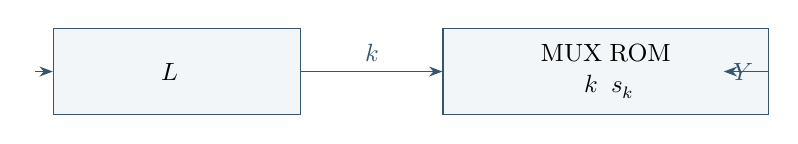
\begin{tikzpicture}[node distance=18mm]
\node[block,text width=29mm] (counter) {模$L$计数器};
\node[block,text width=39mm,right=of counter] (mux) {MUX或ROM\\第$k$项存$s_k$};
\draw[->,ThemeMain] (-1.8,0)--(counter) node[midway,above] {时钟};
\draw[->,ThemeMain] (counter)--(mux) node[midway,above] {$k$};
\draw[->,ThemeMain] (mux)--++(1.5,0) node[right] {$Y$};
\end{tikzpicture}
\end{center}

\subsection{移位寄存器加反馈产生序列}
用 $n$ 位移位寄存器产生长度 $L$ 的周期串时，$2^n\ge L$ 只是必要条件。把循环位串的连续 $n$ 位作为状态窗口；若同一窗口的后续位不同，就不能仅由该窗口决定反馈，须增大 $n$ 或另加状态信息。
\begin{infobox}{例题：00010111序列的反馈设计}
采用三位左移寄存器，状态 $Q_2Q_1Q_0$ 的最高位 $Q_2$ 为输出。
\end{infobox}
\sol 循环窗口为
\[
000\to001\to010\to101\to011\to111\to110\to100\to000.
\]
八个状态两两不同，按 $(Q_2,Q_1,Q_0)^+=(Q_1,Q_0,L_{\mathrm{in}})$，各状态的下一补入位为
\begin{center}
\begin{tabular}{cc cc}
\toprule 状态&$L_{\mathrm{in}}$&状态&$L_{\mathrm{in}}$\\\midrule
000&1&011&1\\001&0&111&0\\010&1&110&0\\101&1&100&0\\\bottomrule
\end{tabular}
\end{center}
以 $Q_2Q_1Q_0$ 为编号，反馈成一项为 $0,2,3,5$，可化简为
\[
L_{\mathrm{in}}=Q_2Q_1'Q_0+Q_2'Q_1+Q_2'Q_0'
=\sum m(0,2,3,5).
\]
因此可用逻辑门实现，也可用八选一将0、2、3、5号数据端接1，其余接0；用74LS138则将对应低有效译码输出经与非门合成。最高位输出依次为 $00010111$。八个三位状态全部在同一循环中，无未用二值状态；任意二值初态对应不同相位，确定相位仍需初始化。

若同一状态窗口重复且后续位相同，可考虑合并，但仍须检查规定周期及相位含义。环形、扭环形适于规则序列；计数器加MUX/ROM适于按索引输出；反馈移位实现依赖窗口能唯一决定下一位。选择方法须同时考虑状态数、资源和所需输出。

\clearpage
\subsection{从反馈装载接线判断稳定模值}
\begin{infobox}{例题：74LS161反馈装载计数器}
2024秋期末回忆版，简答题5。$Q_dQ_cQ_bQ_a=Q_3Q_2Q_1Q_0$，初态0000。计数使能 $EP=ET=1$，并行输入 $DCBA=0000$，异步清零在计数期间不生效；与非门把 $Q_3,Q_2$ 译码到低有效装载端。求稳定状态序列与计数模值。
\end{infobox}
\begin{center}
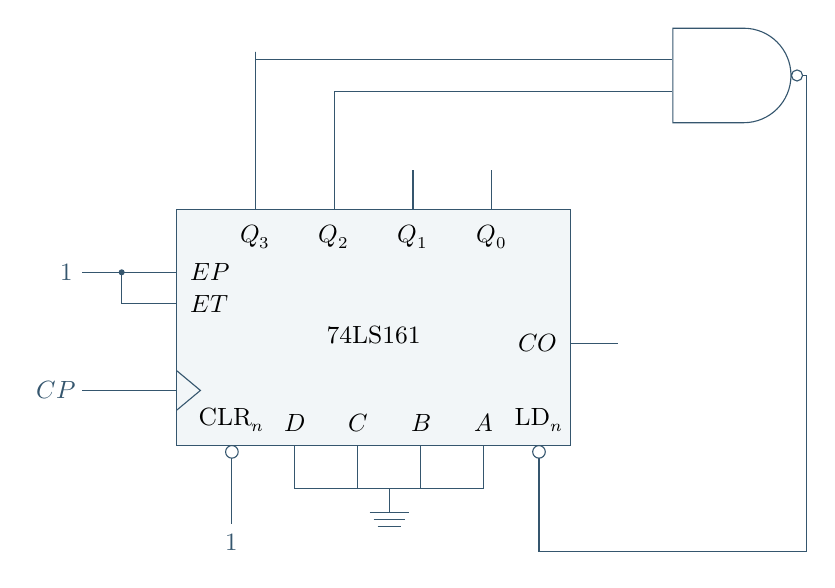
\begin{tikzpicture}[x=10mm,y=10mm,every node/.style={font=\small}]
\draw[ThemeMain,fill=ThemeBack] (3,0) rectangle (8,3);
\node at (5.5,1.4){74LS161};
\foreach \x/\lab in {4/Q_3,5/Q_2,6/Q_1,7/Q_0}
 {\node[below] at (\x,2.93){$\lab$};\draw[ThemeMain] (\x,3)--(\x,3.5);}
\node[right] at (3.05,2.2){$EP$};\node[right] at (3.05,1.8){$ET$};
\draw[ThemeMain] (1.8,2.2) node[left]{$1$}--(3,2.2);
\draw[ThemeMain] (2.3,2.2)--(2.3,1.8)--(3,1.8);
\fill[ThemeMain] (2.3,2.2) circle (1.1pt);
\draw[ThemeMain] (1.8,.7) node[left]{$CP$}--(3,.7);
\draw[ThemeMain] (3,.45)--(3.3,.7)--(3,.95);
\node[left] at (7.95,1.3){$CO$};\draw[ThemeMain] (8,1.3)--(8.6,1.3);
\foreach \x/\lab in {3.7/\mathrm{CLR}_n,4.5/D,5.3/C,6.1/B,6.9/A,7.6/\mathrm{LD}_n}
 {\node[above] at (\x,.05){$\lab$};}
\draw[ThemeMain] (3.7,-.08) circle (.08);
\draw[ThemeMain] (3.7,-.16)--(3.7,-1) node[below]{$1$};
\foreach \x in {4.5,5.3,6.1,6.9}\draw[ThemeMain] (\x,0)--(\x,-.55);
\draw[ThemeMain] (4.5,-.55)--(6.9,-.55);
\draw[ThemeMain] (5.7,-.55)--(5.7,-.85);
\draw[ThemeMain] (5.45,-.85)--(5.95,-.85);
\draw[ThemeMain] (5.5,-.94)--(5.9,-.94);
\draw[ThemeMain] (5.55,-1.03)--(5.85,-1.03);
\node[nand gate US,draw=ThemeMain,logic gate inputs=nn,
 minimum width=13mm,minimum height=12mm] (ng) at (10,4.7) {};
\draw[ThemeMain] (4,3.5)--(4,5.0)|-(ng.input 1);
\draw[ThemeMain] (5,3.5)--(5,4.4)|-(ng.input 2);
\draw[ThemeMain] (7.6,-.08) circle (.08);
\draw[ThemeMain] (ng.output)--(11,4.7)--(11,-1.35)--(7.6,-1.35)--(7.6,-.16);
\end{tikzpicture}
\end{center}
\sol 装载控制的引脚电平是 $\mathrm{LD}_n=(Q_3Q_2)'$。$Q_3Q_2=11$ 时该端为零；其余情况为一。74LS161的并行装载是同步的，须在下一个上升沿读取低有效装载条件。

从0000递增，第一次达到 $Q_3Q_2=11$ 的状态是1100，即十进制12。进入12的那一沿之前，现态为11（二进制1011），装载端仍为一，因此这次正常计数到12。到达12后装载端变为零，下一沿才装入0000：
\begin{center}
\begin{tabular}{c c c l}
\toprule 沿前状态 & $\mathrm{LD}_n$ & 沿后状态 & 本沿动作\\\midrule
1010（10）&1&1011（11）&正常加一\\
1011（11）&1&1100（12）&正常加一\\
1100（12）&0&0000（0）&同步装载零\\\bottomrule
\end{tabular}
\end{center}
所以稳定序列为 $0\to1\to\cdots\to12\to0$，共有13个状态，是模13计数器。1100维持一个完整的稳定计数区间，不能按“达到12就立即清零”误判为模12。其终值 $CO$ 只有在1111且相应使能条件满足时有效；本循环未达到1111，不能直接把 $CO$ 当作模13终值信号。

\begin{infobox}{例题：设计二进制1001至1111循环计数器}
2024秋期末回忆版，简答题7。用74LS161使稳定计数范围为 $1001_2$ 至 $1111_2$，下一沿由1111回到1001。说明并行输入、反馈条件、初态设置与模值。
\end{infobox}
\sol 并行输入须接 $DCBA=1001$。计数允许且清零不生效时，设置
\[
EP=ET=1,\qquad
\mathrm{LD}_n=(Q_3Q_2Q_1Q_0)'=CO'.
\]
最后一项相等依赖 $ET=1$，不能在任意使能条件下照用。电路重绘如下，四输入与非门在1111产生装载低电平：
\begin{center}
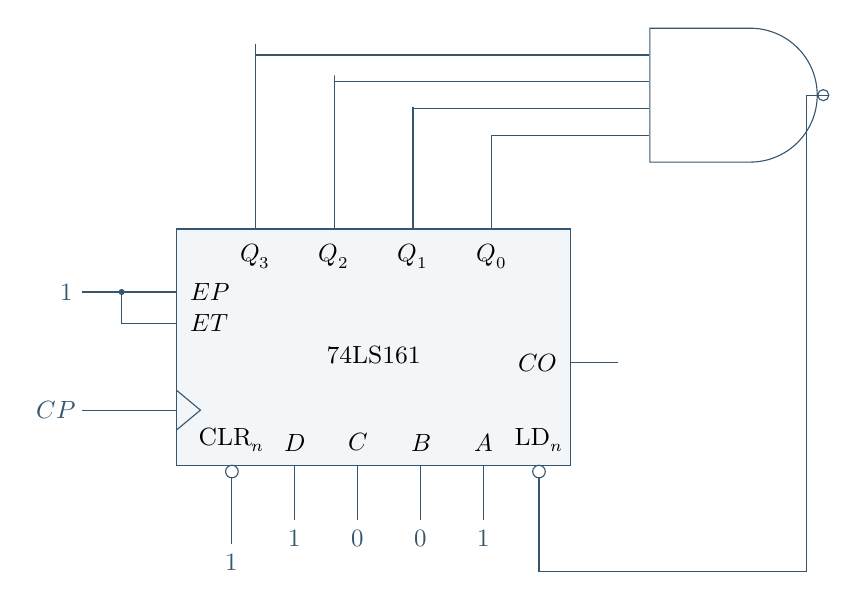
\begin{tikzpicture}[x=10mm,y=10mm,every node/.style={font=\small}]
\draw[ThemeMain,fill=ThemeBack] (3,0) rectangle (8,3);
\node at (5.5,1.4){74LS161};
\foreach \x/\lab in {4/Q_3,5/Q_2,6/Q_1,7/Q_0}
 {\node[below] at (\x,2.93){$\lab$};}
\node[right] at (3.05,2.2){$EP$};\node[right] at (3.05,1.8){$ET$};
\draw[ThemeMain] (1.8,2.2) node[left]{$1$}--(3,2.2);
\draw[ThemeMain] (2.3,2.2)--(2.3,1.8)--(3,1.8);
\fill[ThemeMain] (2.3,2.2) circle (1.1pt);
\draw[ThemeMain] (1.8,.7) node[left]{$CP$}--(3,.7);
\draw[ThemeMain] (3,.45)--(3.3,.7)--(3,.95);
\node[left] at (7.95,1.3){$CO$};\draw[ThemeMain] (8,1.3)--(8.6,1.3);
\foreach \x/\lab in {3.7/\mathrm{CLR}_n,4.5/D,5.3/C,6.1/B,6.9/A,7.6/\mathrm{LD}_n}
 {\node[above] at (\x,.05){$\lab$};}
\draw[ThemeMain] (3.7,-.08) circle (.08);
\draw[ThemeMain] (3.7,-.16)--(3.7,-1) node[below]{$1$};
\foreach \x/\v in {4.5/1,5.3/0,6.1/0,6.9/1}
 {\draw[ThemeMain] (\x,0)--(\x,-.7) node[below]{$\v$};}
\node[nand gate US,draw=ThemeMain,logic gate inputs=nnnn,
 minimum width=13mm,minimum height=17mm] (ng) at (10,4.7) {};
\foreach \x/\y/\k in {4/5.35/1,5/4.95/2,6/4.55/3,7/4.15/4}
 {\draw[ThemeMain] (\x,3)--(\x,\y)|-(ng.input \k);}
\draw[ThemeMain] (7.6,-.08) circle (.08);
\draw[ThemeMain] (ng.output)--(11,4.7)--(11,-1.35)--(7.6,-1.35)--(7.6,-.16);
\end{tikzpicture}
\end{center}
启动时先用外部装载控制使 $\mathrm{LD}_n=0$，在一个上升沿装入1001，然后交给终值反馈；单独异步清零只会装入0000，不能获得要求的初态。正常循环为
\[
1001\to1010\to1011\to1100\to1101\to1110\to1111\to1001,
\]
共有 $15-9+1=7$ 个稳定状态，模值为7。进入1111后还须等待下一有效沿，期间它是有效终值状态。若从0000直接启动，会先经历额外的0至8，不能把这段启动过程说成题设范围内的循环。


\chapterpage{实验资料、代码阅读与验证约定}
\subsection{资料来源与版本对应}
本实验部分依据\href{https://hoa.moe/docs/2025/25Y05/sophomore-autumn/COMP2051}{HOA课程页面}及其链接资料整理。课程页面的路径不是实验年份的证明。资源下载区的\code{labs/2020}包含六次旧版实验；\code{labs/2024/exp3/README.md}包含2024年数码管实验说明。页面“相关实验仓库”链接到\href{https://github.com/capoo-fan/class-experiment/tree/main/数字逻辑电路}{capoo-fan/class-experiment}，其中指导书明确出现2025年的检查日期，且具有六次实验的设计、约束和仿真代码。本部分以这套2025年资料为代码讲解主线，历史版本单列补充。以下要求描述所读取的资料，不表示2026年课程已采用相同题目。
\begin{longtable}{p{0.09\linewidth}p{0.39\linewidth}p{0.42\linewidth}}
\toprule 实验 & 2025年链接仓库 & \code{labs/2020}及2024年补充\\\midrule\endhead
1 & 3--8译码器；四位加减多路复用器 & 拨码开关控制LED；3--8译码器\\
2 & D触发器；八个八位寄存器 & 低有效复位、低有效写使能；结构化寄存器文件\\
3 & 四档频率、双向、按键启停流水灯 & 1秒流水灯；四位格雷码计数器\\
4 & 未消抖/消抖按键计数；0至30循环 & 倒计时、开关值、班级、学号；2024版为0至20饱和计数\\
5 & UART发送\code{hitsz+学号} & Moore/Mealy检测\code{01011}\\
6 & UART收发、最近六字符显示、字符串匹配选做 & 记忆游戏\\\bottomrule
\end{longtable}
\begin{infobox}{注意：开发板和个人信息必须与资料版本对应}
2025年资料的板载100MHz时钟接\code{Y18}；2020年EGO1资料接\code{P17}。复位极性、数码管极性、拨码开关编号和约束文件不能跨板照搬。参考代码中的学号和尾号属于原作者；实际提交时必须替换成使用者本人的信息。尚未给出个人学号，本讲义不编造该信息。
\end{infobox}
\subsection{代码文件与硬件结构}
配套“实验代码/原始参考”按六次实验保留下载到的\code{.v}和\code{.xdc}文件，未经功能改写；“整理示例”放置本讲义的规范化教学示例。原代码和改写示例通过目录及正文说明区分，完整设计代码可在配套文件中查阅。各实验的\code{top}或\code{testbench}名称可能重复，应分别建立工程，不能把全部实验一次加入同一设计。

\term{设计源文件}描述可综合的电路；\term{仿真源文件}产生激励并检查输出；\term{约束文件}指定引脚、电气标准和时钟。\code{always #5 clk = ~clk;}产生仿真时钟；它不生成FPGA内部的晶振。\code{#10}、\code{$display}、\code{$finish}用于测试，不能当作上板电路中的延时方案。实际延时依靠时钟和计数器。

读代码时先确定端口及有效电平，再寻找\code{always @(posedge clk ...)}中的状态，随后读取组合逻辑和模块实例，最后追踪状态更新条件与输出。在一个时钟边沿上，非阻塞赋值\code{<=}先计算右侧旧值，再统一更新左侧；同一边沿工作的多个模块因此可以按寄存器连接关系分析。
\begin{lstlisting}
// A two-stage pipeline: both right-hand sides use old values.
always @(posedge clk) begin
  stage1 <= data_in;
  stage2 <= stage1;
end
\end{lstlisting}
若边沿前\code{stage1=0}、\code{data_in=1}，边沿后\code{stage1=1}而\code{stage2=0}。用\code{=}依次改写两句时，第二句会读取刚改写的\code{stage1}，不能按两级流水线理解。组合过程通常用\code{=}，时钟过程通常用\code{<=}。\code{reg}表示过程变量，完整组合赋值的\code{reg}仍可以综合成组合电路。
\subsection{验证层次与仿真证据}
\term{功能仿真}核对逻辑与时序协议；静态检查核对未声明信号、位宽、锁存器、多驱动及赋值习惯；综合和实现核对资源、时钟、引脚和时序；上板核对实际电平、抖动及连线。功能仿真通过只证明测试激励覆盖到的行为，不能替代后两层。

测试程序宜在\code{negedge clk}改变输入，在\code{posedge clk}之后留出非阻塞赋值更新时间再检查。检查使用\code{!==}可以把\code{x}或\code{z}也作为失败，而普通\code{!=}可能产生未知的条件值。
\begin{lstlisting}
@(negedge clk); en = 1'b1; d = 8'hA5;
@(posedge clk); #1;
if (q !== 8'hA5) $fatal(1, "write failed");
\end{lstlisting}
波形分析应说明“哪个边沿、哪些输入、预期输出、实际输出及依据”。至少覆盖复位、正常路径、暂停或失能、边界和关键失败路径。缩小计数参数可加快仿真，但必须注明缩小比例，上板参数仍按实际100MHz时钟计算。

\chapterpage{Lab 1：组合逻辑与加减多路复用器}
\subsection{要求与文件对应}
2025年实验包括3--8译码器和多路复用器。链接仓库的设计文件\code{mux.v}实现四位加减选择，\code{testbench.v}给出十组激励，\code{pin.xdc}连接开关和LED。译码器在指导书中给出接口与功能表，仓库未提供相应的独立设计文件；后文给出完整教学实现。

多路复用器输入为\code{en}、\code{mux_sel}及两个四位无符号数\code{input_a}、\code{input_b}。失能\code{en=0}时输出\code{4'hF}；使能且\code{mux_sel=0}时相加；使能且\code{mux_sel=1}时相减。四位输出只保留结果低四位。
\begin{lstlisting}
module mux(
  input wire en, mux_sel,
  input wire [3:0] input_a, input_b,
  output reg [3:0] output_c
);
  always @(*) begin
    if (!en) output_c = 4'hF;
    else if (!mux_sel) output_c = input_a + input_b;
    else output_c = input_a - input_b;
  end
endmodule
\end{lstlisting}
\code{always @(*)}表示依赖信号变化后重新计算，三条分支覆盖全部二值控制组合，因此不需要存储旧输出，也不推断锁存器。它不是“先加后减”的执行流程，而是综合成由选择控制的组合数据通路。
\subsection{位宽、溢出与测试输入}
\begin{infobox}{例题：四位运算的实际结果}
\code{input_a=4'hF}、\code{input_b=4'h1}时，加法输出\code{4'h0}。\code{input_a=4'h1}、\code{input_b=4'h2}时，减法输出\code{4'hF}。后一结果表示模16的低四位，不是带负号显示的十进制数。
\end{infobox}
若需保留加法进位，必须扩展输入与输出，例如\code{wire [4:0] total = {1'b0,a} + {1'b0,b};}。实验接口规定四位输出时，丢弃进位符合该接口，不应擅自把端口改成五位。

原仿真声明十位\code{switch}，再按以下连接拆分输入。
\begin{lstlisting}
reg [9:0] switch;
assign {en, mux_sel, input_a, input_b} = switch;
\end{lstlisting}
拼接左侧总宽度为$1+1+4+4=10$，\code{switch[9]}对应\code{en}、\code{switch[8]}对应\code{mux_sel}，其后两组各四位。\code{10'b1_0_1000_0100}表示使能、加法、8、4，结果应为12。下划线只用于可读性，不占位宽。

原十组激励覆盖使能和加减，但没有检查进位截断、负差及全部输入，也没有自动判错。完整穷举包含$2\times2\times16\times16=1024$组，逐组按真值规则计算预期四位结果；配套验证文件完成此检查。
\subsection{3--8译码器与有效电平}
指导书规定\code{en=3'b100}时使能，地址\code{data_in}选中的输出位为0，其余为1；失能时输出全1。这相当于低有效输出译码器，而不能把“选中”一律写成1。
\begin{lstlisting}
module decoder_38(
  input wire [2:0] en, data_in,
  output wire [7:0] data_out
);
  wire active = en[2] & ~en[1] & ~en[0];
  assign data_out = active ? ~(8'b00000001 << data_in)
                           : 8'hFF;
endmodule
\end{lstlisting}
例如地址5时，\code{8'b1 << 5}为\code{8'h20}，取反后\code{data_out=8'hDF}。八位常量确保移位与取反都发生在确定宽度内。2020年指导书的某些示例片段省略使能或输出反相，并把连续赋值输出声明为\code{reg}；完整传统Verilog实现应使用\code{wire}并遵从实际功能表。译码器穷举$8\times8=64$组地址及使能组合。
\subsection{约束、检查与提交内容}
上板验证先检查所有顶层端口都与本板引脚对应，再确认\code{IOSTANDARD}。总线端口在Tcl中使用花括号保护，例\code{[get_ports {input_a[0]}]}；括号中的端口名须与RTL完全相同。组合模块不需要伪造内部时钟。

报告需包含输入输出波形与解释、RTL分析图、综合后电路图。两类图对应不同抽象阶段；综合后结构取决于优化与目标器件，不能仅凭源代码形式断言一定出现某种门或ROM。原约束只可用于相同开发板，换板时需重新核对每个引脚。

\chapterpage{Lab 2：触发器与寄存器文件}
\subsection{D触发器：复位、写入与保持}
2025年\code{dff/dff.v}使用高有效异步复位\code{clr}和高有效同步使能\code{en}，输出为\code{q}。复位无需等待时钟；写入必须在上升沿满足使能；失能时保持。
\begin{lstlisting}
always @(posedge clk or posedge clr) begin
  if (clr) q <= 1'b0;
  else if (en) q <= d;
end
\end{lstlisting}
没有\code{else}表示时钟触发器保持原值。原文件末尾的\code{q <= q;}功能等价但可以省略。\code{d}在两个时钟边沿之间变化不会立即改变\code{q}；复位在边沿之间变为1却会立即清零。异步复位释放在实际硬件中还应满足恢复、移除时序，功能仿真不显示亚稳态。
\subsection{八个八位寄存器与地址选择}
\code{reg8file/reg8file.v}中\code{reg [7:0] regfile [7:0];}声明八个元素，每个元素八位，共64位数据存储。前面的\code{[7:0]}是每个元素的位宽，后面的\code{[7:0]}是数组索引范围。\code{wsel}与\code{rsel}均为三位，分别选择写地址、读地址。
\begin{lstlisting}
reg [7:0] regfile [0:7];
integer i;
always @(posedge clk or posedge clr) begin
  if (clr) begin
    for (i=0; i<8; i=i+1) regfile[i] <= 8'h00;
  end else if (en) regfile[wsel] <= d;
end
assign q = regfile[rsel]; // q is declared as output wire
\end{lstlisting}
该规范化片段把原\code{always @(*) q <= regfile[rsel];}改成连续赋值：读端是组合逻辑，不应额外采用非阻塞更新。异步清零全部元素通常要求触发器资源，不能直接断言这种写法推断出块RAM。

写地址决定哪一个寄存器在时钟边沿接收数据，其余七个保持。读地址改变时，读输出经过组合延迟跟随对应元素，不需要等下一个边沿。读写同址时，边沿前读出旧内容，非阻塞更新后读出新内容；这是本实现的行为，不代表所有RAM端口都如此。
\begin{center}\begin{tabularx}{\linewidth}{c c c Y}
\toprule 操作 & \code{en} & 地址与数据 & 边沿后的结果\\\midrule
复位 & 任意 & \code{clr=1} & 八个元素均为0\\
写入 & 1 & \code{wsel=3,d=A5} & 第3项为\code{A5}\\
保持 & 0 & \code{wsel=3,d=5A} & 第3项仍为\code{A5}\\
读取 & 任意 & \code{rsel=3} & 输出第3项；读不修改存储\\\bottomrule
\end{tabularx}\end{center}
\subsection{2020年结构化要求的独立实现}
旧版规定\code{clrn=0}异步清零，\code{wen=0}同步写入；其中\code{wen}名字未带\code{_n}，但功能表明确低有效。旧版还明确要求实例化译码器、D触发器及多路选择器，不能仅用数组行为描述替代该结构要求。
\begin{lstlisting}
module dffe(input wire clk, clrn, wen, d,
            output reg q);
  always @(posedge clk or negedge clrn)
    if (!clrn) q <= 1'b0;
    else if (!wen) q <= d;
endmodule
module reg8(input wire clk, clrn, wen,
            input wire [7:0] d, output wire [7:0] q);
  genvar b;
  generate for (b=0; b<8; b=b+1) begin: bits
    dffe u_ff(.clk(clk), .clrn(clrn), .wen(wen),
              .d(d[b]), .q(q[b]));
  end endgenerate
endmodule
\end{lstlisting}
再实例化八个\code{reg8}。第$j$项的低有效写使能为\code{we_n[j] = wen | (wsel != j)}，只有总写使能有效且地址匹配时为0。读多路选择器把\code{rsel}指定的八位输出送到\code{q}。配套\code{core_examples.v}给出完整连接。\code{generate}是在 elaboration 阶段展开硬件，八次循环不是运行八拍。

旧指导书建议不约束\code{rsel[2]}以应对开关不足。实际上不能让顶层输入悬空并期待确定值；可以在板级包装模块把该位固定为\code{1'b0}，明确上板只可读取低四个地址，而核心仿真仍验证全部八个地址。
\subsection{验证与易混概念}
至少检查边沿之间异步复位、失能保持、八个地址分别写读、覆盖同址写入及复位后全部清零。原仿真只主要访问地址1和2，不能证明全部地址独立。静态\code{for}复位八项可以展开综合；测试中等待时间、检查循环属于仿真过程。

寄存器文件的写使能只控制写入，不控制读端。\code{en=0}时仍可读取。两套复位和使能的极性必须在端口表和代码中一致，不能只替换变量名。

\chapterpage{Lab 3：可调频率与方向的流水灯}
\subsection{要求与计数参数}
2025年实验要求：100MHz时钟，\code{rst=1}异步复位后仅\code{led[0]}亮；按\code{button}在启动、停止间切换，复位后等待启动；\code{freq_set}选择四档移位频率；\code{dir_set=0}右移、\code{dir_set=1}左移。指导书要求三级寄存器边沿检测，本实验不要求消抖。

令输入频率$f_c=100\,\mathrm{MHz}$、每次移位间隔$T$，一轮计数长度$N=f_cT$。从0数到$N-1$共有$N$个时钟周期，因此终值为$N-1$。
\begin{center}\begin{tabular}{c c c r r}
\toprule \code{freq_set} & 频率 & 间隔 & 周期数$N$ & 终值\\\midrule
\code{00} & 1000Hz & 1ms & 100000 & 99999\\
\code{01} & 100Hz & 10ms & 1000000 & 999999\\
\code{10} & 20Hz & 50ms & 5000000 & 4999999\\
\code{11} & 5Hz & 200ms & 20000000 & 19999999\\\bottomrule
\end{tabular}\end{center}
原文件参数\code{cnt_500hz}实际数值是\code{1_000_000-1}，对应100Hz，应改名为\code{cnt_100hz}以免误读。最大值小于$2^{25}$，25位足够；原26位也正确，只是多留一位。
\subsection{三级采样与启停标志}
\begin{lstlisting}
reg sig_r0, sig_r1, sig_r2;
wire pos_edge = sig_r1 & ~sig_r2;
always @(posedge clk or posedge rst) begin
  if (rst) begin
    sig_r0 <= 0; sig_r1 <= 0; sig_r2 <= 0;
  end else begin
    sig_r0 <= button;
    sig_r1 <= sig_r0;
    sig_r2 <= sig_r1;
  end
end
always @(posedge clk or posedge rst) begin
  if (rst) flag <= 1'b0;
  else if (pos_edge) flag <= ~flag;
end
\end{lstlisting}
输入连续为1并传播到第二级而尚未传播到第三级时，\code{pos_edge}为1；下一拍第三级也为1，脉冲结束。\code{flag}每次上升沿脉冲翻转一次，持续按住不会反复翻转。前两级采样有助于同步异步输入，仍不能消除机械抖动；多个真实上升沿仍可能翻转多次。

原代码没有显式声明\code{pos_edge}，传统Verilog会隐式建立一位\code{wire}。这种隐式声明掩盖拼写错误，整理示例显式声明并使用\code{`default_nettype none}检查未声明连线。
\subsection{终值脉冲和循环移位}
\begin{lstlisting}
wire cnt_end = flag && (cnt >= cnt_max);
always @(posedge clk or posedge rst) begin
  if (rst) cnt <= 0;
  else if (cnt_end) cnt <= 0;
  else if (flag) cnt <= cnt + 1'b1;
end
always @(posedge clk or posedge rst) begin
  if (rst) led <= 8'h01;
  else if (cnt_end) begin
    if (!dir_set) led <= {led[0], led[7:1]};
    else led <= {led[6:0], led[7]};
  end
end
\end{lstlisting}
\code{cnt_end}是单拍时钟使能，不是50\%占空比的新时钟。两段过程都由同一个\code{clk}触发，计数归零与移位使用同一拍边沿前的条件。右循环移位把低位移到最高位，\code{8'h01}变成\code{8'h80}；普通\code{led >> 1}会移入0并丢掉唯一的1，不能替代循环移位。

停止时\code{cnt}和\code{led}保持。再次启动时从剩余计数继续，因此“恢复后第一次移位”不必再等待完整$T$。切换到较短间隔且现值已超过新终值时，\code{>=}使其下一拍归零移位；使用\code{==}可能错过终值。是否切换频率时重置相位是接口约定，原实现选择保留现计数并用大于等于处理。
\subsection{频率含义、仿真与旧版要求}
5Hz表示每秒移位5次，八个位置轮一遍需$8/5=1.6$秒；单个LED重新亮起的周期为八次移位间隔。旧版“其余灯亮过以后再亮”的描述不能误读成相邻两次点亮同一个LED只隔七个总周期。

原仿真把四档周期数缩小1000倍，并用10ns的时钟：第一档每100拍移位一次，间隔1微秒，第二档10微秒，第三档50微秒，第四档200微秒。报告应测量相邻移位的时间差，并明确这不是上板1ms至200ms的真实间隔。

2020版要求独立\code{divider}产生1Hz时钟，再驱动\code{flowLED}，其结构约束与本版单时钟使能方案不同。若采用翻转法得到1Hz、50\%占空比，则每$50\,000\,000$拍翻转一次，终值为\code{49_999_999}；若每$100\,000\,000$拍翻转一次，实际为0.5Hz。生成的新时钟在工程中还需相应时钟约束和正确时钟资源，不能仅看RTL波形。

\chapterpage{Lab 4：数码管扫描、消抖与十进制计数}
\subsection{显示布局和模块划分}
2025版从左到右为\code{DK7}至\code{DK0}：最高两位显示学号末两位；其后两位统计未消抖的\code{S3}上升沿；中间两位统计消抖后的\code{S3}上升沿；最低两位以0.1秒间隔从0数到30，再回0。\code{S2}每按一次在暂停与继续间切换；\code{SW0=0}关闭显示但内部逻辑继续运行；\code{S1=1}异步复位所有时序逻辑。

设计由\code{top.v}、\code{debounce.v}、\code{edge_detect.v}、\code{led_ctrl_unit.v}组成。\code{top.v}分成输入处理、三组计数和显示拼接。\code{led_ctrl_unit}读取32位\code{display}，八个四位字段分别对应八个位置，最后形成\code{led_en}和\code{led_cx}。
\begin{lstlisting}
assign display = {dig7,dig6,dig5,dig4,dig3,dig2,dig1,dig0};
assign led_en = SW0 ? anode_out   : 8'hFF;
assign led_cx = SW0 ? segment_out : 8'hFF;
\end{lstlisting}
位号\code{dig0}位于拼接最右侧、总线最低四位。\code{SW0}只在输出处门控，因而关闭后重新打开可看到计数继续后的新值。这是“关闭显示”，不是“暂停计数”。原学号尾号为48，使用前需替换。
\subsection{动态扫描及段码约定}
\code{refresh_cnt}每100000拍归零并令三位\code{anode_select}加一；每个位置保持1ms，一轮八位为8ms，每位刷新125Hz。三位索引自然从7回0。
\begin{lstlisting}
if (refresh_cnt == time_max) begin
  refresh_cnt <= 0;
  anode_select <= anode_select + 1'b1;
end else refresh_cnt <= refresh_cnt + 1'b1;
\end{lstlisting}
以\code{anode_select=2}为例，选择\code{display[11:8]}，位选为\code{8'b11111011}，仅第2位为0。本版位选低有效，段选按\code{[7:0]={a,b,c,d,e,f,g,dp}}排列，也为低有效。字符0点亮a至f、熄灭g及dp，所以段码为\code{8'h03}；字符7点亮a、b、c，码为\code{8'h1F}。
\begin{center}\begin{tabular}{c*{10}{c}}
\toprule 数字 & 0&1&2&3&4&5&6&7&8&9\\\midrule
段码 & \code{03}&\code{9F}&\code{25}&\code{0D}&\code{99}&\code{49}&\code{41}&\code{1F}&\code{01}&\code{09}\\\bottomrule
\end{tabular}\end{center}
原字符0的旁注\code{8'b1100_0011}与实际\code{8'h03}不一致，应以逐段推导的码值为准。此模块只定义0至9，其他输入默认全灭，适用于本实验十进制显示；要显示A至F，必须补充译码。2020版EGO1段选及板级位选为高有效，并有两组独立段总线，不可照搬本版低有效八位选模板。

理想RTL中同时切换段选、位选不显示路径延迟；上板若有重影，可在换位时先关闭全部位选、更新段码，再启用下一位。消隐拍属于显示时序改进，不改变各位置所对应的数字。
\subsection{连续稳定计数消抖与单次事件}
原消抖模块保存\code{state}作为最近观察到的候选电平，输入不同时更新候选并清计数；连续相同足够久后将候选写入\code{button_out}。100MHz下\code{cnt_max=2_000_000}约为20ms。原计数从0增长到\code{cnt_max}后下一拍才更新输出，准确时刻还包含候选捕获拍；不能宣称恰好2000000拍。

原\code{button_in}直接进入判断逻辑，没有先经过同步寄存器。规范化示例先二级同步，再对同步后的电平作连续稳定计数。
\begin{lstlisting}
if (sync2 == stable) count <= 0;
else if (count == STABLE_CYCLES-1) begin
  stable <= sync2;
  count <= 0;
end else count <= count + 1'b1;
\end{lstlisting}
这里\code{STABLE_CYCLES}为接受一次与当前稳定状态不同的新电平所需的连续周期数。任何一次回到旧稳定值都会清零，短抖动不会通过；释放也必须稳定后才接受。

消抖输出是电平，持续按住期间为1；计数器必须使用该电平的上升沿事件。\code{edge_detect}延迟一拍并比较\code{sig_r0 & !sig_r1}，得到单拍脉冲。若直接\code{if (button_out) count <= count+1;}，持续按住会每个时钟加一。
\subsection{BCD进位与0至30循环}
\term{BCD计数}用独立四位数码保存个位和十位，个位9之后置0并使十位加1。原自动计数在十位3、个位0时归零，因而序列是\code{00,01,...,29,30,00}，共有31个值；一轮为3.1秒。
\begin{lstlisting}
if (tick_100ms && !pause) begin
  if (tens == 4'd3 && ones == 4'd0) begin
    tens <= 0; ones <= 0;
  end else if (ones == 4'd9) begin
    ones <= 0; tens <= tens + 1'b1;
  end else ones <= ones + 1'b1;
end
\end{lstlisting}
原两组按键计数只对个位做9回0，十位一直四位加一，到10以后产生非BCD十位，显示默认熄灭。若约定只显示末两位，须在\code{tens==9 && ones==9}时两位同时回0，形成模100计数。讲义的完整示例明确采用该约定。

原\code{pause}仅阻止数字更新，0.1秒节拍计数继续运行，因此恢复后第一次加一可能不足0.1秒；Lab 3的暂停连同分频计数一起保持，两者的暂停语义不同。报告需解释自身实现，不能只写“计数暂停”。
\subsection{验证范围与版本差异}
仿真至少覆盖八个扫描位置及段码、短毛刺拒绝、两次稳定按下、持续按住一次计数、稳定释放、\code{09 -> 10}进位、\code{29 -> 30 -> 00}、暂停和显示关闭时内部继续计数。\code{SW0=0}时应观察位选全失能而不是\code{display}清零。

2024补充版的布局为“学号尾号、开关中1的个数、消抖按键计数、0至20计数”，不是本版的未消抖计数。其0至20计数到20保持，按\code{S2}重启；重启应同时清数值和0.1秒子计数器，避免首个间隔不足0.1秒。人口计数用逐位累加得到0至8，4位输出足够，累加中间结果须采用足够位宽。2020版则显示倒计时、开关十六进制值、班级和学号，并要求两个指定小数点常亮。

\chapterpage{Lab 5：UART发送与字符串调度}
\subsection{实验要求与帧格式}
2025版要求9600波特率、三段式状态机，不断发送\code{hitsz+个人学号}。两个字符串发送之间至少等待0.2秒，同一字符串中相邻字符发送间隔不超过0.01秒。\code{S1}为高有效异步复位。仓库\code{uart_send.v}实现单字节发送，\code{top.v}调度15个ASCII字符并等待；该15字符长度来自原作者十位学号，实际学号长度变化时需同步改末地址与指针位宽。

\term{UART}使用独立于系统时钟的串行位时序。此处采用\code{8N1}：空闲1、起始位0、8个数据位、无校验、停止位1，数据最低位先发。一个字节占10个位周期。
\begin{lstlisting}
// Frame order in time: start, data[0],...,data[7], stop.
wire [9:0] frame = {1'b1, data, 1'b0};
// frame[0] is transmitted first.
\end{lstlisting}
发送ASCII字符\code{'A'}时数据为\code{8'h41}，实际八个数据位按时间为\code{1,0,0,0,0,0,1,0}。发送十六进制数\code{8'h0A}不等于发送两个字符\code{'0'}、\code{'A'}；后者须发送\code{8'h30}与\code{8'h41}两个字节。
\subsection{波特率计数与状态转移}
100MHz系统时钟下，每位周期数取
\[
N_b=\left\lfloor\frac{100\,000\,000}{9600}\right\rfloor=10416,
\qquad f_b=\frac{100\,000\,000}{10416}\approx9600.614\ \mathrm{bit/s}.
\]
相对9600的误差约0.0064\%。从0数到10415，因此原\code{cnt_max=10415}正确。注释“10417”与该实现不符，应统一为10416拍。
\begin{center}\begin{tabularx}{\linewidth}{l Y Y}
\toprule 状态 & 输出或动作 & 离开条件\\\midrule
\code{IDLE} & 输出1；接受\code{valid}并锁存\code{data} & 请求有效后进入\code{START}\\
\code{START} & 输出0，起始位 & 一个\code{baud_tick}后进入\code{DATA}\\
\code{DATA} & 输出\code{data_buf[bit_cnt]} & 每个位末位号加一；位7结束进入\code{STOP}\\
\code{STOP} & 输出1，停止位 & 一个位周期后回\code{IDLE}\\\bottomrule
\end{tabularx}\end{center}
状态寄存器用时钟过程更新\code{current_state}；组合过程根据\code{current_state}、\code{valid}、\code{baud_tick}和\code{bit_cnt}产生\code{next_state}；输出过程产生\code{dout}。三段式描述强调职责分离，输出过程是否寄存还需明确，不能凭块数直接判定Moore或Mealy。
\begin{lstlisting}
if (current_state == IDLE && next_state == START)
  data_buf <= data;
\end{lstlisting}
这条锁存使发送期间外部\code{data}改变不影响当前帧。原\code{dout}根据旧现态在边沿上寄存，所以相对于\code{current_state}改变延后一拍；数据位号也在同一边沿更新，输出读取旧位号。逐拍跟踪时必须包括这拍延迟，不能只读状态图便宣称输出在状态跳转的同一拍已改变。
\subsection{字符串ROM与顶层调度}
\code{top.v}以\code{pointer}访问\code{string_rom}，\code{case}为每个地址给出ASCII。它是组合查表，不是按时钟逐行执行。三个调度状态为\code{send_char}、\code{wait_char}和\code{s_delay}。在发送状态产生单拍\code{uart_valid}，等待一个字符帧时间后推进指针，最后一个字符后进入0.2秒等待。

一个字符帧约为$10\times10416/100\,000\,000=1.0416$毫秒，15字符约15.624毫秒；再等待0.2秒，字符串轮次约为0.215624秒，另有调度拍开销。\code{char_wait_max=10*10416}用于估算忙碌时长，但固定等待必须与发射器的请求采样、输出延迟严格一致。
\begin{infobox}{方法：用完成反馈推进发送}
更清晰的接口为\code{valid}、\code{ready}、\code{busy}、\code{done}：只在\code{valid && ready}的边沿接受字节；发送完成时给出单拍\code{done}；字符串调度器收到\code{done}再推进\code{pointer}。这样位周期改变时无需在顶层重新估算十个位的计时。课程指定接口不能改时，可增加内部完成信号或保留经验证的等待逻辑，并明确接口限制。
\end{infobox}
原接口没有\code{ready/busy}。\code{valid}在非\code{IDLE}状态出现时会被忽略；持续拉高则可能在回到空闲时重复发送。因此一次请求应只高一拍，并由上层保证当前可以接受。
\subsection{测试程序的边界与报告内容}
原测试用例包括\code{A5}、\code{3C}、\code{FF}、\code{00}、\code{5A}，逐位比较起始、数据及停止位。原测试按以下表达式计算等待参数：
\begin{lstlisting}
localparam DIVIDER = CLOCK_FREQ / BAUD_RATE - 1;
\end{lstlisting}
RTL每位实际10416拍，测试每次却等待10415拍；短帧可能仍通过，但比较时刻会逐位提前。规范测试应以实际位长计时，在每位中心采样。

除原用例外，应验证输入数据在帧内改变、忙碌时请求、相邻帧边界、发送期间复位及字符串间隔。报告给出完整一帧、现态/次态、位计数、波特率计数、锁存数据和串行输出，而不能只展示\code{FF}连续高电平。

\chapterpage{Lab 6：UART接收、显示与字符串匹配}
\subsection{必做要求与顶层连接}
2025版必做内容为9600波特率收发：接收电脑端ASCII字符并在数码管显示最近六个字符，不足六个时高位全灭；剩余两位显示接收字符累计数的末两位；按\code{S3}一次发送一次个人学号，按键需消抖；\code{S1}为异步复位。指导书规定顶层只做实例化和模块连接，复杂功能放入子模块。

原\code{top.v}实例化下表所列模块。
\begin{center}\begin{tabularx}{\linewidth}{l Y}
\toprule 模块 & 功能\\\midrule
\code{debounce, edge_detect} & 按键稳定过滤与单次事件\\
\code{uart_recv} & 串行帧接收，输出数据与有效事件\\
\code{display_logic} & ASCII译码、最近六字符和累计数\\
\code{led_ctrl_unit} & 八位扫描及空白字符显示\\
\code{send_ctrl} & 按键请求后的字符串发送调度\\
\code{string_match} & 前缀状态机与回复字符请求\\
\code{mux} & 两条发送位流的模式选择\\\bottomrule
\end{tabularx}\end{center}
接收数据一路进入显示、另一路进入匹配；两套发送输出经\code{SW0}选择送往\code{uart_tx}。
\begin{center}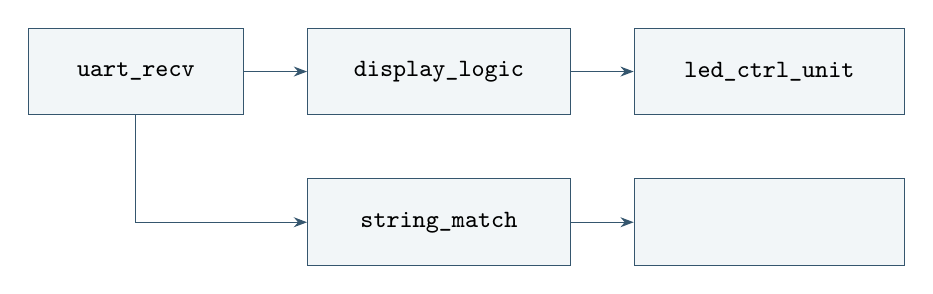
\begin{tikzpicture}[node distance=8mm]
\node[block,text width=25mm] (rx) {\code{uart_recv}};
\node[block,text width=31mm,right=of rx] (disp) {\code{display_logic}};
\node[block,text width=32mm,right=of disp] (scan) {\code{led_ctrl_unit}};
\node[block,text width=31mm,below=of disp] (match) {\code{string_match}};
\node[block,text width=32mm,right=of match] (tx) {发送选择与输出};
\draw[->,ThemeMain] (rx)--(disp);
\draw[->,ThemeMain] (disp)--(scan);
\draw[->,ThemeMain] (rx)|-(match);
\draw[->,ThemeMain] (match)--(tx);
\end{tikzpicture}\end{center}
原\code{send_ctrl}发送的是\code{hitsz+原作者学号}，而本实验必做要求为“个人学号”。Lab 5的前缀不能直接当成Lab 6的要求；交付前应移除前缀或明确验证方接受的格式，并替换个人数据。
\subsection{接收状态机与位中心采样}
接收引脚是异步输入，应先二级同步。原\code{uart_recv.v}直接用\code{din}判断和采样，功能仿真可能正常，硬件仍有亚稳态传播风险；同步不会消除亚稳态本身，但可以降低其传播概率。

接收四态为\code{IDLE}、\code{START}、\code{RECV}、\code{STOP}。空闲检测到0进入起始态；等待半位并再次检查0，以拒绝短低电平毛刺；然后每隔一整位采一个数据位；最后在停止位中点检查1，输出数据和单拍\code{valid}。
\begin{center}\begin{tabular}{c c c}
\toprule 相对起始下降沿时刻 & 采样内容 & 位位置\\\midrule
$0.5T_b$ & 起始位复核 & 应为0\\
$1.5T_b$ & 第一个数据位 & \code{data[0]}\\
$2.5T_b$至$8.5T_b$ & 后续七位 & \code{data[1]}至\code{data[7]}\\
$9.5T_b$ & 停止位 & 应为1\\\bottomrule
\end{tabular}\end{center}
表中$T_b=10416$个系统周期；实际实现增加同步和检测延迟，通常仅若干系统拍，远小于一个串行位。原\code{START && cyc_half}清零计数，故接收状态每次\code{cyc_flag}发生在下一数据位的中点，而不是数据边界；需要以起始沿为基准累加时间理解。

原接收器到停止位时间就输出\code{valid}，没有确认\code{din==1}，无法拒绝坏停止位。规范化\code{uart_clean.v}先同步，并验证停止位，坏帧只复位接收过程、不拉高有效信号。只对帧有效的数据更新显示和计数。
\subsection{ASCII译码、六字符移位与空白编码}
\code{display_logic.v}用\code{case(recv_data)}把\code{'0'}至\code{'9'}和\code{'A'}至\code{'F'}转换成十六进制数码，同时兼容小写a至f；其他字符令\code{valid_char=0}。处理条件为\code{valid && valid_char}，因此原代码仅统计可显示字符。指导书只测试0至F，但累计“接收到的字符个数”的范围仍需约定；本讲义采用所有帧有效字节计数、仅可显示字符进入六槽显示，以便区分物理接收与显示过滤。

普通十六进制值占四位，却没有额外码表示空白。原代码每槽用五位，\code{5'h1F}表示全灭；\code{0_0000}至\code{0_1111}表示0至F。八槽拼接形成40位\code{display_data}，不同于Lab 4的32位。
\begin{lstlisting}
if (valid && valid_char) begin
  slots[5] <= slots[4]; slots[4] <= slots[3];
  slots[3] <= slots[2]; slots[2] <= slots[1];
  slots[1] <= slots[0]; slots[0] <= {1'b0,hex_out};
end
\end{lstlisting}
非阻塞赋值保证每个槽取得旧的右邻字符，新字符进入\code{slots[0]}。复位时六槽全部为空白。连续接收\code{1,2,A}后，高位仍为空白，低端显示\code{12A}；不能把空白初始化为数字0。

原\code{recv_count}为八位，从255加一回0。即使显示时取\code{recv_count / 10}再模10，以及\code{recv_count}模10，第256个字符仍会显示00而非56。要只显示累计计数的末两位，应直接模100计数或用两位BCD，明确\code{99 -> 00}，这样任意长度输入都保留正确末两位。
\subsection{字符串匹配：前缀状态与输入事件}
选做一要求检测\code{start}、\code{stop}、\code{hitsz}并分别回复ASCII\code{'1'}、\code{'2'}、\code{'3'}；未匹配回复\code{'0'}；必须用状态机且可连续测试。仓库选择这项，未提供选做二矩阵键盘计算器的设计代码。本讲义只整理已有实现及其正确性，不编造不存在的计算器代码。

\code{string_match.v}有13个状态：初始态，\code{s,st,sta,star,start}，\code{sto,stop}，\code{h,hi,hit,hits,hitsz}。状态表示已读字符后缀与目标前缀的匹配长度；\code{valid=0}时保持，不应在每个100MHz时钟把同一个字符重复读入。
\begin{lstlisting}
if (valid) begin
  case (current_state)
    star_state: if (recv_data == "t" || recv_data == "T")
                  next_state = start_state;
    sto_state:  if (recv_data == "p" || recv_data == "P")
                  next_state = stop_state;
    hits_state: if (recv_data == "z" || recv_data == "Z")
                  next_state = hitsz_state;
    // Full code supplies fallback transitions for every input.
  endcase
end
\end{lstlisting}
此片段只展示成功边，不是可独立使用的完整组合过程。原完整代码还有\code{s/S}、\code{h/H}重起前缀等失败转移；每个输入都必须给出次态。失败不能一律归初始，例如读到\code{hists...}等含可继续前缀的输入时须保存实际后缀。

匹配输出属于Mealy事件：\code{current_state=star_state}且当前有效字符为\code{t}时，就产生回复\code{'1'}，不必等进入\code{start_state}再读一个新字符。\code{flag}记录本行已有成功匹配，行终结字符到来时如未匹配才回复\code{'0'}。
\subsection{终结符、忙碌反馈与模式切换}
任意长度输入在尚未终结前不能判定“未匹配”。原代码以\code{CR=8'h0D}或\code{LF=8'h0A}为终结。若电脑发送\code{CRLF}，\code{CR}清除\code{flag}后紧跟\code{LF}，可能为已成功的行额外产生一次\code{'0'}请求；若发射器恰好忙碌，这次请求又可能被丢弃。两种缺陷会掩盖彼此，不能据串口只看到一个字节判断正确。

明确的策略是以\code{LF}结束一行而忽略\code{CR}，或把\code{CRLF}合并成一个终结事件。若仍选择单\code{CR}终结，测试软件必须采用该约定，并测试连续行、空行和一行多个命中。

原匹配器的回复请求直接送入没有\code{busy}反馈的\code{uart_send}。在上一回复发送中产生的请求会丢失。规范化设计将回复字符入队，只在发送器\code{ready}时出队；有限队列须定义满时行为。更基本的替代是按实验约定限制输入节奏，并在讲义和测试中明确该限制，不能暗称可处理任意速率连续命中。

顶层\code{SW0}直接多路选择两个独立发送器的位流，若在一帧中途切换可能截断帧。合理方案是在空闲时锁存模式，并由一个公共发送器服务两个请求源；若保留原代码，模式只应在两发送器空闲时改变。
\subsection{完整验证路径}
接收先通过原十组字节用例，再测试短起始毛刺、坏停止位、背靠背帧和帧中复位。显示测试空白、1至6字符、第7字符挤出旧字符、大小写、非法字符及255/256字符计数边界。发送测试短抖动、长按只发一次、第二次按键、忙碌请求与学号内容。匹配测试三个关键词、大小写、噪声前缀、连续输入、未匹配行、\code{CRLF}及发送拥塞。

每个测试应同时检查数据和有效事件，既防止“数值正确但重复接收”，也防止“有脉冲但数据错误”。报告的结构图应标出每个模块的时钟、复位、有效信号与数据方向；顶层连接正确不等于各子模块的接口时序已匹配。

\chapterpage{历史Lab补充：格雷计数、序列检测与记忆游戏}
\subsection{格雷码计数器}
2020年Lab 3第二题要求四位格雷码循环计数，仅仿真，观察内部二进制计数和格雷输出并覆盖复位、使能。设四位二进制状态为\code{binary}，格雷码为\code{binary ^ (binary >> 1)}。
\begin{lstlisting}
always @(posedge clk_i or negedge rst_n_i)
  if (!rst_n_i) binary <= 4'h0;
  else if (en_i) binary <= binary + 1'b1;
assign gray_o = binary ^ (binary >> 1);
\end{lstlisting}
二进制\code{3 -> 4}对应\code{0011 -> 0100}，多个二进制位变化；格雷码为\code{0010 -> 0110}，仅一位变化。\code{15 -> 0}对应\code{1000 -> 0000}，循环边也只变一位。逐项测试相邻码异或是否为独热值，同时检查\code{en_i=0}保持。

格雷码并不消除亚稳态。组合转换\code{binary ^ (binary >> 1)}可能因二进制触发器延迟不同而产生毛刺；跨时钟域使用时常把格雷结果寄存后同步，并满足相应路径约束。课程中的理想码表性质与真实物理波形需区分。
\subsection{01011序列：状态意义及转移表}
2020年Lab 5要求分别设计Moore及Mealy检测器，检查八位字内是否含\code{01011}；\code{set_i}开始新检测，结果命中后保持到下一次开始。需锁存输入字、明确从最高位至最低位输入状态机，并仅消耗八位，不把前一字后缀接到下一字前缀。

令\code{S0}表示无匹配前缀，\code{S1,S2,S3,S4}分别表示已匹配\code{0,01,010,0101}。Mealy转移表如下，\code{hit}仅在读最后一个1时有效：
\begin{center}\begin{tabular}{c c c c}
\toprule 现态 & 输入0次态 & 输入1次态 & 命中条件\\\midrule
\code{S0} & \code{S1} & \code{S0} & 无\\
\code{S1} & \code{S1} & \code{S2} & 无\\
\code{S2} & \code{S3} & \code{S0} & 无\\
\code{S3} & \code{S1} & \code{S4} & 无\\
\code{S4} & \code{S3} & \code{S0} & 输入1\\\bottomrule
\end{tabular}\end{center}
\code{S4}遇0得到\code{01010}，其中最长可继续的目标前缀后缀为\code{010}，故回\code{S3}，不能一律回\code{S1}。\code{01011}末尾没有非空目标前缀后缀，命中后回\code{S0}。Moore增加\code{S5}表示完整命中，其输出为1；\code{S5}遇0去\code{S1}、遇1去\code{S0}。

Mealy的瞬时命中为\code{(state==S4) && bit_valid && bit_in}；Moore命中为\code{state==S5}。输出若寄存，须说明对应的采样边沿。字级持久结果可用\code{detect_o <= detect_o | hit;}，新\code{start}优先清零；Moore在最后一位命中时须保留一拍完成态或根据最终次态捕获，不能在处理位7的边沿立即强制回初态而丢失命中。

验证全部256个字并与软件规则“八位字符串含\code{01011}”比较，其中原指定\code{11011111}为不命中，\code{01010111}命中。串行附加题每个消抖\code{set_i}事件接收一位，命中计数只在接受事件上加一；显示一位数时必须明确超过9后的处理。
\subsection{记忆游戏：需求拆解与数据格式}
2020年Lab 6要求复位显示八个0；\code{S0}启动生成五个互不相同的五位八进制数并存储，以1秒间隔播放；\code{S1}进入按地址查看；\code{S2}进入匹配输入；\code{S3}每次确认采样\code{SW[2:0]}；\code{S4}复位。五位八进制数用15位表示，每一位八进制数占3位。数码管十六进制译码仍可显示0至7。

生成的五个数彼此不同，不要求一个数内部五个数码都不同。示例\code{44444}因此合法。可采用自由运行计数器采样或非零种子的LFSR产生候选，候选写入前与已经保存的0至$k-1$项逐项比较，重复则重新生成；不能只用不同地址便宣称数据互异。上电固定种子的固定取样时序可能每次给出相同五项，应按题意让启动时刻影响取样，并记录不属于密码学随机源。

控制流程可设\code{WAIT_START -> GENERATE -> PLAY -> WAIT_VIEW -> VIEW -> MATCH}。\code{PLAY}保存播放索引和1秒计数，每满1秒推进一项；第5项显示满1秒后保持并等待\code{S1}。输入模块保存最近五个八进制数码，每次确认事件更新窗口：
\begin{lstlisting}
wire [14:0] candidate_window = {window[11:0], sw[2:0]};
if (confirm_pulse) begin
  window <= candidate_window;
  // Compare candidate_window, not the old window.
end
\end{lstlisting}
若在同一时钟过程更新\code{window}后用\code{window}比较，非阻塞语义会比较旧窗口，结果晚一位。还需记录已经输入的数量，未满五位之前不得以初始化的前导零误报匹配。
\subsection{旧指导书中的地址与闪烁歧义}
五项按示例分别编号0至4，输入\code{03}读取第四项\code{17531}；因此有效地址应为\code{0 <= address < 5}。指导书却写“地址大于5时显示F”，没有定义地址5，并与五项存储的范围不一致。本讲义按五项、零起始编号统一采用\code{address >= 5}为非法，显示八个F；若当年教师另有地址约定应按明确补充修改。

显示“地址--匹配数”可统一为八个字符，例如\code{4--44444}，两条短横线占两位。题目示例只写一条短横，剩余位未指定；本讲义以八位布局明确处理，不能将此排版选择当作唯一官方格式。

匹配失败显示八个以4Hz闪烁的0。若4Hz指完整亮灭周期，则半周期0.125秒，在100MHz下每12500000拍翻转亮灭，终值\code{12_499_999}；若每0.25秒翻转则完整闪烁为2Hz。报告应明确采用的定义。每次\code{S3}均可继续更新窗口和匹配，成功后也不能锁死而阻止下一次输入。
\subsection{模块接口与验证安排}
建议划分按键同步消抖、周期节拍、候选生成及去重、五项存储、游戏控制、五位滑动匹配、显示编码和扫描。所有模块统一采用同一系统时钟，低速行为以时钟使能驱动。跨模块事件用单拍脉冲，数据在事件有效的边沿被接收。

验证应检查五项互异、数值15位宽和种子规则、五次播放顺序及时间、所有有效/非法地址、恰满五位时首次匹配、连续滑窗成功与失败、闪烁完整周期，以及每个状态中复位都回等待态。存储写入后立即读取时需注意实现的读延迟，不用仿真无限等待掩盖接口未定义。

本历史综合题没有在所读取2020资料中提供完整RTL答案；上述是依据指导书整理的设计与关键代码，不冒称原作者已完成的工程。2025综合题的原始代码则在配套目录完整保留。

\chapterpage{主要结论与术语}
\subsection{核心公式与适用条件}
\begin{longtable}{p{0.23\linewidth}p{0.69\linewidth}}
\toprule 内容 & 结论及条件\\\midrule\endhead
按位计数 & $N=\sum d_ir^i$；数符范围与基数一致\\
二进制到格雷 & 最高位不变，其余 $g_i=b_{i+1}\oplus b_i$\\
标准表达式 & $F=\sum m(\mathcal O)=\prod M(\mathcal Z)$；固定变量次序，成一与成零编号互补\\
德摩根 & $(A+B)'=A'B'$，$(AB)'=A'+B'$；反号作用范围明确\\
香农展开 & $F=XF_1+X'F_0=(X'+F_1)(X+F_0)$\\
卡诺圈 & $2^k$格合法圈消去$k$个变量；圈1读与或，圈0读或与\\
静态冒险 & 指定两级结构下，相邻目标格需由共同项覆盖；单输入变化判据\\
全加器 & $S_i=a_i\oplus b_i\oplus C_{i-1}$；$C_i=a_ib_i+(a_i\oplus b_i)C_{i-1}$\\
全减器 & $D_i=a_i\oplus b_i\oplus B_{i-1}$；$B_i=a_i'b_i+a_i'B_{i-1}+b_iB_{i-1}$\\
MUX & $Y=\sum m_k(\symbf S)I_k$；编号由选择端位序决定\\
ROM与LUT & $n$输入、$b$输出ROM需$2^n b$位；$k$输入一位LUT有$2^k$表项\\
奇偶校验 & 偶校验位为数据归约异或，奇校验位为其反；检出奇数位翻转\\
触发器 & SR：$Q^+=S+R'Q,SR=0$；D：$Q^+=D$；JK：$Q^+=JQ'+K'Q$；T：$Q^+=T\oplus Q$\\
时钟使能 & $Q^+=CE\cdot D+CE'Q$；禁用时保持\\
计数器 & $N$是稳定循环的状态数；$n$触发器最多$2^n$状态\\
反馈截断 & 从0计数：异步清零译码$M$，同步归零通常译码$M-1$\\
二进制状态编码 & $k\ge\lceil\log_2N\rceil$；最少状态位不等于最少总逻辑\\
Mealy与Moore & Mealy输出依赖现态和输入，Moore输出只依赖现态\\\bottomrule
\end{longtable}

\subsection{常用符号与术语}
\begin{longtable}{p{0.25\linewidth}p{0.67\linewidth}}
\toprule 符号或术语 & 本讲义的含义\\\midrule\endhead
$A',Q'$ & 逐位逻辑取反；不是次态\\
$Q^+$ & 次态；课件也记$Q^{n+1}$或$Q^*$\\
$AB,A+B$ & 与、或；HDL分别用\code{&}、\code{|}\\
$\oplus,\odot$ & 异或、同或\\
$m_i,M_i$ & 编号$i$的最小项、最大项，$M_i=m_i'$\\
$d_i,\times$ & 不完全给定函数的无关项，具体符号结合上下文识别\\
MSB、LSB & 最高、最低有效位；明确位宽和位序\\
$C_{i-1},C_i$ & 全加器的输入、输出进位；外部最低输入为$C_{-1}$\\
$B_{i-1},B_i$ & 全减器的输入、输出借位\\
$P_i,G_i$ & 超前进位中的传递、产生函数；本讲义$P_i=a_i\oplus b_i$\\
$CE,EN,LD$ & 时钟使能、一般使能、装载控制；有效极性须单独规定\\
下标$n$与小圆圈 & 常用来标识低有效控制，但最终以功能表为准\\
$RCO$ & 进位/终值或级联信号，波形定义依器件\\
$X,Z$与\code{x,z} & 大写可作普通变量名；HDL小写值分别为未知、高阻\\
RTL、FSM & 寄存器传输级、有限状态机\\
SIPO、PISO & 串入并出、并入串出\\
PLD、CPLD、FPGA & 可编程逻辑器件、复杂PLD、现场可编程门阵列\\\bottomrule
\end{longtable}

\subsection{知识联系与易混概念}
数制确定数量的解释，编码确定对象与码字的对应；真值表确定组合函数，标准式保证描述完整，卡诺图与布尔代数减少实现项数；译码器产生最小项，MUX实现按选择条件展开，ROM/LUT直接存储真值表。

时序电路在组合逻辑之外增加状态存储。触发器特征方程把驱动函数变成次态函数，激励表把期望次态变成可实现的驱动。寄存器强调保存和传送，计数器强调固定状态循环，状态机强调受输入控制的状态变化。序列检测处理输入历史，序列发生器按内部状态产生输出。

逻辑真值相同与瞬态波形相同须分开；同步计数与同步清零须分开；使能保持与禁用清零须分开；驱动高阻与主动驱动零须分开；化简无关项与仿真未知须分开。状态可自启动不代表初相位固定，也不保证恢复期间的输出正确。

\subsection{实验主要结论与代码术语}
\code{wire}用于连接，\code{reg}用于过程赋值；边沿过程表示时序状态，完整\code{always @*}表示组合规则；\code{=}与\code{<=}必须按求值时序解释。连续稳定过滤解决机械抖动，同步链降低异步输入的亚稳态传播风险，边沿检测把稳定电平变为单次事件，三者作用不同。

从0计数的长度为终值加一。移位频率、完整LED循环频率、方波翻转频率和完整亮灭频率不可混用。\code{tick}通常是原时钟域的单拍使能。扫描索引决定数码位置，译码表决定段形状，有效电平由具体板卡规定。

UART一帧的八位数据最低位先传，ASCII字符与十六进制数值需区分。\code{valid}表示当前边沿有一份可接受的数据，不能当作持续请求。发送忙碌反馈、接收停止位验证、末两位计数以及字符串终结符，决定连续运行的边界行为。状态代表已接受输入的历史，输入无效时保持状态。

\subsection{本次实验验证记录与边界}
整理示例使用Icarus Verilog进行自动功能仿真：四位加减器1024组、译码器64组、两种寄存器文件八个地址及异步复位保持、Moore与Mealy检测器各256个字、格雷循环32次转移、四拍节拍、短毛刺拒绝与长按单次事件、模100计数256次；改写UART逐字节验证全部256种发送数据和全部256种接收数据，并验证短起始毛刺、坏停止位拒绝及随后恢复。

原UART发送测试五组数据、接收测试十组数据均通过。原测试程序以\code{byte}命名任务参数，使用传统Verilog模式可运行，若按SystemVerilog编译则与关键字冲突；不能把这一语言模式错误当成UART逻辑错误。原Lab 4、5、6的顶层完成语法与展开检查。

额外定向仿真确认原接收显示累计256个有效字符后显示00，而低两位应为56；成功匹配\code{start}后收到\code{CRLF}会提出\code{31}与\code{30}两次回复请求，后者为额外零回复。原始文件未改写，这些问题在正文和配套说明中标出。整理示例的验证只涉及所列模块和范围；未在Vivado中综合、布局布线或上板，不宣称全部参考工程已通过硬件验收。2020年记忆游戏为需求与设计解析，没有原始完整RTL可验证。

\subsection{课件范围与资料说明}
新增例题参考《2024秋数逻期末回忆版》（资料标注更新日期2024年11月25日）与上述课件。电路图按可辨认接线重绘，逐项列出输入条件、位序、有效电平和初态；改编题注明补充条件。地址译码题的位序与通常74LS138约定冲突，正文分别给出两种解释；波形设计题重新规定明确的周期与初态。回忆资料未能确认的细节不据此补写为原题条件。

本讲义以桌面“数字逻辑设计课件”文件夹内全部15份PDF为主要依据。重复版本合并为13个课件主题，保留较长版本中的补充内容，按知识联系整合为前述章节。课件中的教学安排、考核比例、建议和课堂投票不作为学科正文重复收录。
\begin{longtable}{>{\raggedright\arraybackslash}p{0.24\linewidth}p{0.44\linewidth}p{0.23\linewidth}}
\toprule 课件标识 & 内容 & 对应正文\\\midrule\endhead
01 引言 & 基本概念、数字系统、设计层次 & 第1章\\
02 数制和编码 & 位权、进制转换、BCD、余3、格雷、字符编码 & 第2章\\
03-1 逻辑代数 & 逻辑门、真值表、定律、反演、对偶、代数化简 & 第3章\\
03-2 布尔代数应用 & 标准式、最大最小项、不完全给定函数 & 第3、4章\\
03-3 卡诺图 & 多变量图、读式、无关项、代码转换 & 第4、5章\\
03-4 险象及消除 & 延迟、冒险、判别与消除 & 第6章\\
04-1 组合逻辑设计 & 表决、运算、加减器、三态门 & 第7章\\
04-2 常用组合器件 & 译码、MUX、编码、校验、比较、ROM、PLD & 第8、9章\\
05 Verilog HDL & 模块、数据类型、运算、赋值、过程、仿真 & 第9章\\
06-1 时序元件 & 锁存器、触发器、附加控制、类型转换 & 第10章\\
06-2 寄存器与计数器 & 寄存器、移位、计数、节拍、HDL & 第11章\\
06-03 同步时序设计 & 状态图、状态化简、编码、序列检测 & 第12章\\
06-04 中规模芯片应用 & 计数器、级联、寄存器、序列发生器 & 第13章\\\bottomrule
\end{longtable}
04-2的65页与68页版本合并，后者补充的优先编码、奇偶校验及分组比较Verilog应用均纳入对应主题。06-2的两个47页版本提取内容一致，仅保留一套讲解。讲义中的小规模算术、码制转换、反馈状态及序列例子按定义逐值核对；硬件延迟与非法控制条件未用理想真值表替代。

必要纠正包括：标准ASCII为七位；十个数码从16个码字中任选一组共有 $\binom{16}{10}=8008$ 种选集，而给十个数码分别分配不同码字有 $16!/6!$ 种映射，二者不同；锁存器可带异步复位，完整赋值与过程类型决定是否推断锁存器；FSM不必有终态；状态位下界须使用向上取整；同步计数的组合译码仍可能有毛刺；74LS193清零高有效、74LS190/191级联端功能不同；若未给出适用统计模型，不将“单比特错误占96\%”当作通用概率。

外部核验仅用于澄清标准、器件极性和明显错误，未扩展课件学科范围。可核对前文链接的RFC与TI原厂资料，以及\href{https://www.intel.com/content/www/us/en/docs/programmable/683082/22-2/register-and-latch-coding-guidelines.html}{Intel寄存器与锁存器编码指南}。器件图引脚名称、端口次序、有效电平和允许同时控制条件应按具体型号的数据手册执行。
\subsection{实验资料与代码归档}
实验资料读取时间为2026年10月4日。2025年六次实验的要求来自课程页面链接仓库中各次“实验指导书”PDF，设计来自“源代码”目录；报告只用于辅助核对，不用报告结论替代RTL与功能表。2020年指导书与2024年补充取自\href{https://github.com/HITSZ-OpenAuto/COMP2051/tree/main/labs}{HOA课程仓库labs}。配套目录记录原始下载路径及SHA-256摘要，可区分原文件与规范化示例。

后续资料到来时，先确定实验版本、开发板、接口及任务变化，再在本讲义最新源文件中更新相应章节和验证记录，保留已有理论内容及统一样式。不能把另一学年的题目直接覆盖成同名实验的唯一要求。
\end{document}
